% $Id: msk-014-user.tex 9730 2021-12-21 20:25:11Z mskala $

%
% MSK 014 user/build manual
% Copyright (C) 2022  Matthew Skala
%
% This program is free software: you can redistribute it and/or modify
% it under the terms of the GNU General Public License as published by
% the Free Software Foundation, version 3.
%
% This program is distributed in the hope that it will be useful,
% but WITHOUT ANY WARRANTY; without even the implied warranty of
% MERCHANTABILITY or FITNESS FOR A PARTICULAR PURPOSE.  See the
% GNU General Public License for more details.
%
% You should have received a copy of the GNU General Public License
% along with this program.  If not, see <http://www.gnu.org/licenses/>.
%
% Matthew Skala
% https://northcoastsynthesis.com/
% mskala@northcoastsynthesis.com
%

\documentclass{ncmanual}

% \usepackage{bigstrut}
% \usepackage{dcolumn}
\usepackage{lilyglyphs}
\usepackage{musicography}
\usepackage{rotating}
\usepackage{stfloats}
\usepackage{tikz}

\usetikzlibrary{arrows.meta,calc,decorations,decorations.pathmorphing,patterns}

\newcommand{\blinkcodeLR}[4]{\begin{tikzpicture}[scale=0.6]
  \node at (-0.5,1) {L};
  \node at (-0.5,0) {R};
  \draw (0,-0.5) -- (0,1.5);
  \draw (8,-0.5) -- (8,1.5);
  \draw (0,0) -- (8,0);
  \draw (0,1) -- (8,1);
  \foreach \x/\y in {#1} {
    \draw[fill=green] (\x,0.65) rectangle (\y,1.35);
  }
  \foreach \x/\y in {#2} {
    \draw[fill=red] (\x,0.65) rectangle (\y,1.35);
  }
  \foreach \x/\y in {#3} {
    \draw[fill=green] (\x,-0.35) rectangle (\y,0.35);
  }
  \foreach \x/\y in {#4} {
    \draw[fill=red] (\x,-0.35) rectangle (\y,0.35);
  }
\end{tikzpicture}}

\newcommand{\blinkcodeX}[2]{\begin{tikzpicture}[scale=0.6]
  \node at (-0.71,0) {};
  \draw (0,-0.5) -- (0,0.5);
  \draw (8,-0.5) -- (8,0.5);
  \draw (0,0) -- (8,0);
  \foreach \x/\y in {#1} {
    \draw[fill=green] (\x,-0.35) rectangle (\y,0.35);
  }
  \foreach \x/\y in {#2} {
    \draw[fill=red] (\x,-0.35) rectangle (\y,0.35);
  }
\end{tikzpicture}}

\title{MSK~014\quad Gracious Host\\User/Build Manual}
\author{Matthew Skala}
\date{\today}

\begin{document}

\maketitle

%%%%%%%%%%%%%%%%%%%%%%%%%%%%%%%%%%%%%%%%%%%%%%%%%%%%%%%%%%%%%%%%%%%%%%%%

\begin{copyrightpage}
Hardware documentation for the MSK~014\\
Copyright \copyright\ 2022 Matthew Skala

\GPLThreeStatement
\end{copyrightpage}

\tableofcontents

%%%%%%%%%%%%%%%%%%%%%%%%%%%%%%%%%%%%%%%%%%%%%%%%%%%%%%%%%%%%%%%%%%%%%%%%

\texdependspdfworkaround

% $Id: general.tex 6473 2018-11-30 15:28:26Z mskala $

%
% MSK 009 general notes
% Copyright (C) 2018  Matthew Skala
%
% This program is free software: you can redistribute it and/or modify
% it under the terms of the GNU General Public License as published by
% the Free Software Foundation, version 3.
%
% This program is distributed in the hope that it will be useful,
% but WITHOUT ANY WARRANTY; without even the implied warranty of
% MERCHANTABILITY or FITNESS FOR A PARTICULAR PURPOSE.  See the
% GNU General Public License for more details.
%
% You should have received a copy of the GNU General Public License
% along with this program.  If not, see <http://www.gnu.org/licenses/>.
%
% Matthew Skala
% https://northcoastsynthesis.com/
% mskala@northcoastsynthesis.com
%

\chapter{General notes}

This manual documents the MSK~009 Coiler Multi-Mode Filter and Rectifier,
which is a module for use in a Eurorack modular synthesizer.  The module
contains a voltage-controlled two-pole state variable filter
implemented using inductors (coils, hence the name) as the main
energy-storing components in the integrators.  It also uses capacitors,
which have their main effect at bass frequencies, with the filter's
behaviour shading from capacitor-based to inductor-based between about 500Hz
to 2kHz.  There are separate outputs for high-pass, band-pass, and low-pass
transfer functions, and two audio inputs, one of which goes through a
full-wave rectifier before being fed into the filter.

\section{Controls and connections}

The front panel of the module is shown in Figure~\ref{fig:panel-mockup}.

\begin{figure}
{\centering\setlength{\fboxsep}{0pt}\setlength{\fboxrule}{0.6pt}%
\fbox{\includegraphics{panel-mockup.pdf}}\par}
\caption{Module front panel.}\label{fig:panel-mockup}
\end{figure}

\subsection{TUNE knob}

This knob adjusts the overall frequency of the filter, for all three
outputs.  Its setting is added to the control voltage inputs.  It should
cover the entire usable range of the filter, with a little bit of excess at
the low end to allow for ``closing'' the filter more completely when using
voltage control in a low-pass gate patch.

\subsection{res knob}

This sets the ``resonance'' of the filter by attenuating one of the feedback
paths.  Counterclockwise for a flatter response curve, clockwise for a
sharper peak.  Near the clockwise maximum resonance, the filter will
oscillate.  Because of the way the inductors respond differently to phase at
different points on the audio spectrum, this knob's effect interacts with
the current frequency setting; the height of the resonance peak and the
point at which oscillation begins will change with the cutoff frequency,
creating a wide range of varying-timbre effects.

\subsection{att knob}

This is an attenuator for the CV2 input---the lower of the two CV inputs, to
which this knob is joined by the zigzag resistor line in the panel art,
symbolizing attenuation.  With the knob fully clockwise the sensitivity of
this input is approximately 1V/octave, the same as the unattenuated input. 
At lower settings, the CV2 input is less sensitive.

\subsection{IN inputs}

Audio inputs to the filter.  The upper input, marked with a diode symbol and
the notation \textbf{fw rect}, is subjected to full-wave rectification
(positive and negative voltages translated into their absolute values)
before being applied to the filter.  The lower input is a direct connection. 
Both inputs may be used at once; their effects are summed.

The rectified input includes a phase inverter (both positive and negative
voltages are translated into \emph{negative}) to cancel out the
naturally-occuring phase inversion between the
input and LP output in this filter topology.  As a result, if you feed an
audio signal into the rectified input with the filter cutoff significantly
below the frequency of the audio, it will be rectified and filtered into a
\emph{positive} voltage tracking the overall amplitude of the input signal. 
This way the module can be used as an envelope follower.

The inputs can accept any voltages between the module's power rails ($-$12V
to $+$12V) without damage.  The module my be overdriven, creating
significant distortion, with inputs beyond about $\pm$5V.

\subsection{CV inputs}

Exponential control voltages for filter cutoff frequency.  The upper socket
(CV1) has a nominal sensitivity of 1V/octave; but the tracking of this
filter is not meant to be very accurate, and it cannot be made highly
accurate because of the somewhat unpredictable properties of the inductors. 
Tracking will differ in different parts of the audio spectrum.  The
CV-processing circuit is partially temperature-compensated, with
zeroth-order ``offset'' compensation but not first-order ``tracking''
compensation.  The lower socket's (CV2) sensitivity is adjustable with the
att knob, to a maximum of the same sensitivity as CV1.  The CV1 input,
attenuated CV2 input, and TUNE knob setting are all summed to produce the
control value for the filter core.

Both CV inputs can accept voltages anywhere between the module's power rails
($-$12V to $+$12V) without damage.  Which voltages are useful depends on the
patch and the setting of the TUNE knob, but a typical user might aim for 0V
to 5V.

\subsection{HP, BP, and LP outputs}

These are the three outputs of the filter core:  high-pass, band-pass, and
low-pass.  Because this is a two-pole filter, the asymptotic slopes of the
response curves are 12dB/octave for the high-pass and low-pass, and
6dB/octave on each of two slopes for the band-pass.

All three outputs are active simultaneously, driven by the combined input
from the two IN jack sockets.  The phase relationships among the three
outputs will change with frequency as the filter shifts between using its
capacitors and its inductors; that means mixing outputs to produce other
filter functions (such as notch filtering) may produce results that sound
good, but they are unlikely to be strong on measures like stopband
attenuation.

Voltage levels on the audio outputs will normally be similar to the voltage
levels on the inputs, with the maximum possible voltage limited by possible
clipping in the op amp chips at around $\pm$10V.  Output level at maximum
oscillation will be about $\pm$5V.  At the lowest resonance setting, the BP
output will be a little quieter than the other two, an effect which tends to
disappear at higher resonance.

\section{Specifications}

The nominal input impedance is 100k$\Omega$ for all inputs except the
rectifier input, which varies between 50k$\Omega$ and 100k$\Omega$.  Nominal
output impedance is 1k$\Omega$ for all outputs.

Any voltage between the power supply rails (nominally $\pm$12V) is safe for
the module, on any input; output voltages are limited by the capabilities of
the op amps to about $\pm$10V and will clip if the inputs are driven
sufficiently hard.  Distortion resulting from limiting in internal feedback
paths may show up before the outputs actually clip.

The circuit is DC-coupled throughout; as a result, it can operate at very
low frequencies, but small DC offsets may appear on the outputs.  Trimmers
are provided for minimizing offset effects.

Briefly shorting any input or output to any fixed voltage at or between the
power rails, or shorting two to each other, should be harmless to the
module.  Patching the MSK~009's output into some other module's output
should be harmless to the MSK~009, but doing that is not recommended because
it is possible the non-MSK~009 module may be harmed.

This module (assuming a correct build using the recommended components) is
protected against reverse power connection.  It will not function with the
power reversed, but will not cause or suffer any damage.  Some other kinds
of power misconnection may possibly be dangerous to the module or the power
supply.

In normal operation the maximum current demand of this module is 25mA from
the +12V supply and 25mA from the -12V supply.  Placing an unusually heavy
load on the outputs (for instance, with so-called passive modules) can
increase the power supply current beyond those levels.

\section{Voltage modification}

This circuit is designed for $\pm$12V power.  It should work acceptably on
$\pm$15V power without modification, assuming all components are rated for
the increased voltage, but some current levels and adjustment ranges are
related to the power supplies and so just applying $\pm$15V power with no
changes may not give optimal results.  In particular, I would expect doing
that to create ``dead zones'' at the ends of the tuning control range.  My
suggestion if using $\pm$15V power would be to increase all four
220k$\Omega$ resistors (R5, R8, R19, and R29) to 270k$\Omega$; that should
restore the intended current levels and adjustment ranges.

I have calculated but not tested these resistor changes.

\section{Source package}

A ZIP archive containing source code for this document and for the module
itself, including things like machine-readable CAD files, is available from 
the Web site at 
\url{https://northcoastsynthesis.com/}.  Be aware that actually building
from source requires some manual steps; Makefiles for GNU Make are provided,
but you may need to manually generate PDFs from the CAD files for inclusion
in the document, make Gerbers from the PCB design, manually edit the .csv
bill of materials files if you change the bill of materials, and so on.

Recommended software for use with the source code includes:
\begin{itemize}
  \item GNU Make;
  \item \LaTeX\ for document compilation;
  \item LaTeX.mk (Danjean and Legrand, not to be confused with other
    similarly-named \LaTeX-automation tools);
  \item Circuit\_macros (for in-document schematic diagrams);
  \item Kicad (electronic design automation);
  \item Qcad (2D drafting); and
  \item Perl (for the BOM-generating script).
\end{itemize}

The kicad-symbols/ subdirectory contains my customised schematic symbol and
PCB footprint libraries for Kicad.  Kicad doesn't normally keep dependencies
like symbols inside a project directory, so on my system, these files
actually live in a central directory shared by many projects.  As a result,
upon unpacking the ZIP file you may need to do some reconfiguration of the
library paths stored inside the project files, in order to allow the symbols
and footprints to be found.  Also, this directory will probably contain some
extra bonus symbols and footprints not actually used by this project,
because it's a copy of the directory shared with other projects.

The package is covered by the GNU GPL, version 3, a copy of which is
included in the file COPYING.

\section{PCBs and physical design}

The enclosed PCB design is for two boards.  Board 1 is
3.90$''$\linebreak[0]$\times$\linebreak[0]1.50$''$ or
99.06mm\linebreak[0]$\times$\linebreak[0]38.10mm.  Board 2 is a little
shorter,
3.40$''$\linebreak[0]$\times$\linebreak[0]1.50$''$ or
86.36mm\linebreak[0]$\times$\linebreak[0]38.10mm.
The two boards are intended to
mount in a stack parallel to the Eurorack panel, held together with M3
machine screws and male-female hex standoff hardware.  See
Figure~\ref{fig:panel-stack}.  Including 18mm of clearance for the mated
power connector, the module should fit in 46mm of depth measured from the
back of the front panel.

\begin{figure}
{\centering
\begin{tikzpicture}[scale=0.1]
  \path[draw=black,dashed,thick] (27.2,-44.14) rectangle (45.2,-24.14);
  \path[draw=black,fill=black!30!white] (-2.0,-64.25) rectangle (0,64.25);
  \path[draw=black,fill=white] (0,-30.48) rectangle (13,-24.48);
  \path[draw=black,fill=white] (0,30.48) rectangle (13,24.48);
  \path[draw=black,fill=blue!50!white] (13,-49.53) rectangle (14.6,49.53);
  \path[draw=black,fill=white] (14.6,-30.48) rectangle (25.6,-24.48);
  \path[draw=black,fill=white] (14.6,30.48) rectangle (25.6,24.48);
  \path[draw=black,fill=blue!50!white] (25.6,-45.72) rectangle (27.2,40.64);
  \path[draw=black,fill=white] (27.2,-30.48) rectangle (29.2,-24.48);
  \path[draw=black,fill=white] (27.2,30.48) rectangle (29.2,24.48);
  \path[draw=black,fill=black!10!white] (29.2,-28.98) rectangle (31.2,-25.98);
  \path[draw=black,fill=black!10!white] (29.2,28.98) rectangle (31.2,25.98);
  \node at (6.5,38) {\parbox{10mm}{\centering \small 13mm standoff}};
  \node at (20.1,38) {\parbox{11mm}{\centering \small 11mm standoff}};
  \node at (13,64) {\small 2mm front panel};
  \node at (21.4,58.5) {\small 2$\times$ 1.6mm PCBs};
  \draw[>=latex',->,very thick] (13.8,56.7) -- (13.8,50.53);
  \draw[>=latex',->,very thick] (26.4,56.7) -- (26.4,41.64);
  \node at (36.2,-34.14)
    {\parbox{17mm}{\centering \small 18mm clearance for mated power connector}};
  \draw (45.2,-48) -- (45.2,-64);
  \draw[>=latex',<->,thick] (0,-56) -- (45.2,-56);
  \node[fill=white] at (23.0,-56) {\small $\approx$46mm depth};
\end{tikzpicture}\par}
\caption{Assembled module, side view.}\label{fig:panel-stack}
\end{figure}

\section{Use and contact information}

This module design is released under the GNU GPL, version 3, a copy of which
is in the source code package in the file named \texttt{COPYING}.  One
important consequence of the license is that if you distribute the design to
others---for instance, as a built hardware device---then you are obligated
to make the source code available to them at no additional charge, including
any modifications you may have made to the original design.  Source code for
a hardware device includes without limitation such things as the
machine-readable, human-editable CAD files for the circuit boards and
panels.  You also are not permitted to limit others' freedoms to
redistribute the design and make further modifications of their own.

I sell this and other modules, both as fully assembled products and
do-it-yourself kits, from my Web storefront at
\url{http://northcoastsynthesis.com/}.  Your support of my business is what
makes it possible for me to continue releasing module designs for free. 
The latest version of this document and the associated source files can be
found at that Web site.

Email should be sent to\\ \url{mskala@northcoastsynthesis.com}.

% $Id: nonusb.tex 9713 2021-12-18 19:22:35Z mskala $

%
% Non-USB operation
% Copyright (C) 2022  Matthew Skala
%
% This program is free software: you can redistribute it and/or modify
% it under the terms of the GNU General Public License as published by
% the Free Software Foundation, version 3.
%
% This program is distributed in the hope that it will be useful,
% but WITHOUT ANY WARRANTY; without even the implied warranty of
% MERCHANTABILITY or FITNESS FOR A PARTICULAR PURPOSE.  See the
% GNU General Public License for more details.
%
% You should have received a copy of the GNU General Public License
% along with this program.  If not, see <http://www.gnu.org/licenses/>.
%
% Matthew Skala
% https://northcoastsynthesis.com/
% mskala@northcoastsynthesis.com
%

\chapter{Non-USB operation}

\begin{figure*}[b]
{\centering
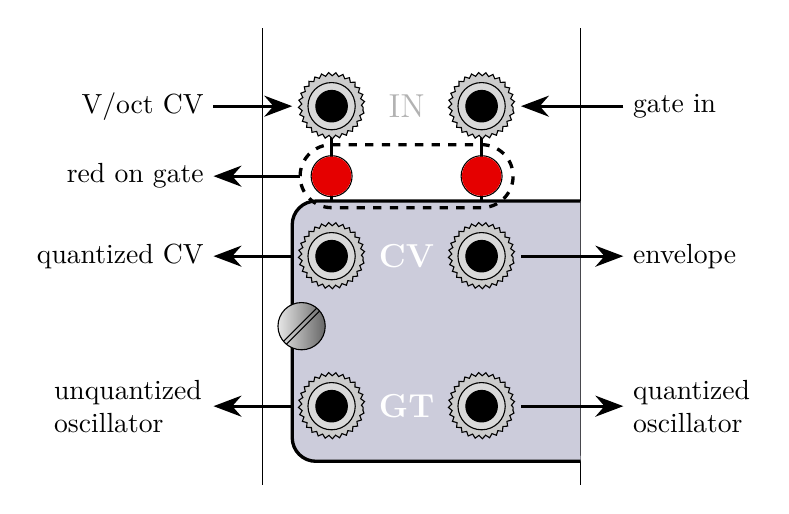
\begin{tikzpicture}
  {\setmainfont[Path={../../tsukurimashou/otf/},
BoldFont={TsukurimashouBokukkoExtraBoldPS}]{TsukurimashouBokukkoDemiboldPS}%
% start out defining coordinates
\coordinate (lbh) at (4.91mm,31.23mm) {};
\coordinate (j1) at (8.72mm,59.17mm) {};
\coordinate (j2) at (27.77mm,59.17mm) {};
\coordinate (j3) at (8.72mm,40.12mm) {};
\coordinate (j4) at (27.77mm,40.12mm) {};
\coordinate (j5) at (8.72mm,21.07mm) {};
\coordinate (j6) at (27.77mm,21.07mm) {};
\coordinate (d5) at (8.72mm,50.28mm) {};
\coordinate (d6) at (27.77mm,50.28mm) {};
%
\draw (0,11.07mm) -- (0,69.07mm);
\draw (40.30mm,11.07mm) -- (40.30mm,69.07mm);
%
\draw[very thick,black] (j1) -- (j3);
\draw[very thick,black] (j2) -- (j4);
\draw[very thick,black,fill=blue!30!black!20!white,rounded corners=3.0mm]
  (40.30mm,47.12mm) -- (3.72mm,47.12mm) --
  (3.72mm,14.07mm) -- (40.33mm,14.07mm);
\node[black!30!white] at ($(j1)!0.5!(j2)$) {\large IN};
\node[white] at ($(j3)!0.5!(j4)$) {\large\textbf{CV}};
\node[white] at ($(j5)!0.5!(j6)$) {\large\textbf{GT}};
%
% board-to-panel mounting holes, to clear M3 machine screw
\draw (lbh) circle[radius=1.60mm];
% six jacks with M6 threads, 6.3mm holes
\draw (j1) circle[radius=3.15mm];
\draw (j2) circle[radius=3.15mm];
\draw (j3) circle[radius=3.15mm];
\draw (j4) circle[radius=3.15mm];
\draw (j5) circle[radius=3.15mm];
\draw (j6) circle[radius=3.15mm];
% two LEDs, 5.20mm holes
\draw (d5) circle[radius=2.60mm];
\draw (d6) circle[radius=2.60mm];
%
% mock up screw heads, knobs
% machine screws with 6mm heads
\foreach \screwname in {lbh} {
  \path[draw=black,shading=ball,
    left color=black!10!white,right color=black!60!white]
    (\screwname) circle[radius=3mm];
  \draw ($(\screwname)+(50:3.0mm)$)--($(\screwname)+(220:3.0mm)$);
  \draw ($(\screwname)+(40:3.0mm)$)--($(\screwname)+(230:3.0mm)$);
}
% jacks with knurled nuts
\foreach \jackname in {j1,j2,j3,j4,j5,j6} {
  \path[draw=black,fill=black!20!white,
    decorate,decoration={snake,amplitude=0.6,segment length=2.5}]
    ($(\jackname)+(0,-0.15mm)$) circle[radius=4mm];
  \path[draw=black,fill=black!15!white] (\jackname) circle[radius=3mm];
  \path[draw=black,fill=black] (\jackname) circle[radius=2mm];
}
}

%
  \path[fill=red!90!black] (d5) circle[radius=2.50mm];
  \path[fill=red!90!black] (d6) circle[radius=2.50mm];
  \draw[very thick,-{Stealth[scale=1.2]}]
    ($(j1)+(-15mm,0)$) -- ($(j1)+(-5mm,0)$);
  \draw[very thick,-{Stealth[scale=1.2]}]
    ($(j2)+(18mm,0)$) -- ($(j2)+(5mm,0)$);
  \draw[very thick,{Stealth[scale=1.2]}-]
    ($(d5)+(-15mm,0)$) -- ($(d5)+(-4mm,0)$);
%  \draw[very thick,{Stealth[scale=1.2]}-]
%    ($(d6)+(18mm,0)$) -- ($(d6)+(4mm,0)$);
  \draw[rounded corners=4mm,very thick,dashed]
    ($(d5)+(-4mm,-4mm)$) rectangle ($(d6)+(4mm,4mm)$);
  \draw[very thick,{Stealth[scale=1.2]}-]
    ($(j3)+(-15mm,0)$) -- ($(j3)+(-5mm,0)$);
  \draw[very thick,{Stealth[scale=1.2]}-]
    ($(j4)+(18mm,0)$) -- ($(j4)+(5mm,0)$);
  \draw[very thick,{Stealth[scale=1.2]}-]
    ($(j5)+(-15mm,0)$) -- ($(j5)+(-5mm,0)$);
  \draw[very thick,{Stealth[scale=1.2]}-]
    ($(j6)+(18mm,0)$) -- ($(j6)+(5mm,0)$);
%
  \node[anchor=east] at ($(j1)+(-15mm,0)$) {V/oct CV};
  \node[anchor=west] at ($(j2)+(18mm,0)$) {gate in};
  \node[anchor=east] at ($(d5)+(-15mm,0)$) {red on gate};
  \node[anchor=east] at ($(j3)+(-15mm,0)$) {quantized CV};
  \node[anchor=west] at ($(j4)+(18mm,0)$) {envelope};
  \node[anchor=east] at ($(j5)+(-15mm,0)$)
    {\parbox{19mm}{unquantized oscillator}};
  \node[anchor=west] at ($(j6)+(18mm,0)$)
    {\parbox{15mm}{quantized oscillator}};
\end{tikzpicture}\par}
\caption{Jack/LED functions for non-USB mode.}\label{fig:non-usb-jacks}
\end{figure*}

The Gracious Host is meant to work with a USB device like a MIDI controller,
but as a default, with no USB device connected, the standard firmware will
function as a baby synth voice.  See Figure~\ref{fig:non-usb-jacks} for the
panel jack assignments in this mode.

The left CV input is volt per octave pitch, with a nominal range from 0V for
MIDI note 36 (C two octaves below Middle C, 65.406Hz) to 5V for MIDI note
96 (C three octaves above Middle C, 2093.004Hz).  The right CV input is for
a gate signal (threshold approximately 1.62V).  Both LEDs will light, in red,
when the gate is high.

The left CV output is a semitone quantized version of the CV input.  The
right CV output is an ADSR envelope with fixed parameters.  And the two
digital outputs are square wave oscillators:  unquantized pitch on the left,
quantized pitch on the right.

\newpage

The unquantized oscillator runs only while
the gate is high, whereas the quantized oscillator runs continuously once
started.  The concept here is that you could use the module with an external
VCA and the quantized and envelope outputs to get sound during the decay tail, or just
use the unquantized output directly and have a very basic synth voice in the
Gracious Host alone.

Note that the digital outputs, as usual, produce only the fixed levels of 0V
for low and approximately 9V for high; so the square waves on these outputs
include a DC offset of approximately 4.5V.

If you connect a USB device, the module will leave this mode and attempt to
do something appropriate to the device instead.

% $Id: midi.tex 9713 2021-12-18 19:22:35Z mskala $

%
% MIDI interface
% Copyright (C) 2022  Matthew Skala
%
% This program is free software: you can redistribute it and/or modify
% it under the terms of the GNU General Public License as published by
% the Free Software Foundation, version 3.
%
% This program is distributed in the hope that it will be useful,
% but WITHOUT ANY WARRANTY; without even the implied warranty of
% MERCHANTABILITY or FITNESS FOR A PARTICULAR PURPOSE.  See the
% GNU General Public License for more details.
%
% You should have received a copy of the GNU General Public License
% along with this program.  If not, see <http://www.gnu.org/licenses/>.
%
% Matthew Skala
% https://northcoastsynthesis.com/
% mskala@northcoastsynthesis.com
%

\chapter{MIDI interface}

The Gracious Host's MIDI subsystem handles connections to USB MIDI devices
like (musical) keyboards, DIN-to-USB cables, and synthesizers.  The same
backend also processes MIDI events generated by the typing (QWERTY) keyboard
driver.

%%%%%%%%%%%%%%%%%%%%%%%%%%%%%%%%%%%%%%%%%%%%%%%%%%%%%%%%%%%%%%%%%%%%%%%%

\section{USB compatibility}

The usual pattern with USB standards is that the governing organization
defines a complicated protocol intended to capture every possible strange
feature that an unusual device might support; and a simplified version
representing the lowest common denominator.  Then most implementors just use
the simplified version, and the few who are building unusual devices that
really require a complicated protocol, ignore the official one anyway and
make up their own proprietary interfaces to use instead, which they don't
document, so you can only access those devices through reverse engineering
or with the manufacturers' proprietary drivers and on the operating systems
they support.  USB MIDI is no exception.

The Gracious Host will work with most \emph{class compliant} USB MIDI
devices in the real world.  Technically, that means USB devices which expose
an interface of class 1 subclass 3 and one BULK IN endpoint for MIDI stream
data.  Things like DIN MIDI to USB cables, controller keyboards, and so on,
are likely to work.  The Gracious Host is only intended to receive, not
send, MIDI data from the USB port, so USB devices like synthesizers will
probably work to the extent they can be used as MIDI controllers, but not as
synthesizers per se.  Devices that combine multiple
synthesizers, audio interfaces, MIDI ports, and other things in a single
product, are iffy.

Devices that are not \emph{class compliant} will not work.  In particular, a
device that requires a special software driver of its own to work with a
personal computer and cannot be used with a PC operating system's generic
driver for that category of device, is likely not to work with the Gracious
Host.

The Roland UM-ONE DIN to USB MIDI cable has a switch on it for ``TAB'' or
``COMP.'' The vendor documents this switch as selecting whether you want to
plug it into a ``tablet'' or a ``computer,'' but what it really does is it
selects class compliance:  in ``TAB'' mode the cable is class compliant and
will work with the Gracious Host, and in ``COMP'' mode it isn't and won't. 
So you should always use it in ``TAB'' mode with the Gracious Host.  I think
requiring a manual selection between the two interfaces (instead of exposing
them both for automatic selection through the USB auto-configuration
mechanism) is certainly a violation of the spirit, and maybe also the
letter, of the USB standards on Roland's part.  Other devices probably have
similar issues, so if you are trying to connect some device similar in
nature to a UM-ONE and find it doesn't work with the Gracious Host, try
looking for any kind of compatibility mode switch or similar configuration
setting, and change it.

I have an Akai MPK Mini keyboard that is basically class compliant, except
it sends 64 bytes of apparently random garbage through the MIDI interface
every time it boots up.  The Gracious Host will ignore that burst, as well
as any similar behaviour from other devices.  I'm not sure Akai still sells
this product anymore, and if they do, it may well be that the current
version has been updated not to send bursts of garbage.

The Gracious Host does not support the new features introduced in USB MIDI
2.0.  Since all USB MIDI 2.0 class compliant devices are required to also
support USB MIDI 1.0 connections, the new version should not create any
compatibility problems with the Gracious Host.  The USB MIDI 2.0 standard
does remove some of the special features of USB MIDI 1.0 for complicated
devices that the Gracious Host did not support anyway (and, it's clear,
almost nobody supported).

%%%%%%%%%%%%%%%%%%%%%%%%%%%%%%%%%%%%%%%%%%%%%%%%%%%%%%%%%%%%%%%%%%%%%%%%

\section{General comments on MIDI}

The Gracious Host's function is usually determined by the channel of the
most recent MIDI event it has received.  The channels are not fully
independent and, with the exception of pairs designed to work together like
Channels~8 and~9, it usually will not work well to send messages to multiple
channels at once.  Some data structures in the firmware are shared, so you
may find for instance that changing the pitch bend on Channel~1 also has the
effect of changing it on Channel~3.

The Gracious Host supports only those MIDI messages that are directly
relevant to its functions as described in this documentation.  Some features
of MIDI not relevant to the Gracious Host, like Omni Mode, System Exclusive
messages, and so on, will be ignored even if the MIDI organization has
declared them mandatory.

Running Status is supported.

Pitch Bend messages are supported, and the range is $\pm$2 semitones by
default.  Support for adjustable pitch bend range (MIDI Registered Parameter
Number 0) is planned but not yet implemented.

New features of MIDI~2.0 are not supported.

The Gracious Host (regardless of channel mode) will process the MIDI Timing
Clock message, which defines a 24 PPQN clock, in order to set the tempo used
for things like the arpeggiator channels.  This clock is also available on
an output jack, or similar clocks are accepted on input jacks, in some
channel modes; and when using a typing keyboard (described in the next
chapter) the Scroll Lock LED blinks in time with the MIDI clock and the
keypad Insert key can be used as a tap tempo input.  The module will process
the MIDI Start message as a reset to the start of the current quarter note,
but it ignores other MIDI sequencer-control messages (Stop, Continue, Song
Position Pointer, and Song Select).

%%%%%%%%%%%%%%%%%%%%%%%%%%%%%%%%%%%%%%%%%%%%%%%%%%%%%%%%%%%%%%%%%%%%%%%%

\section{Channel 1:  mono CV/gate with velocity and square wave}

In this mode the Gracious Host can control a single channel of a CV/gate
synthesizer.  Note On and Off messages translate to pitch and velocity
control voltages with a nominal 0V to 5V range representing MIDI notes 36 to
96 with any relevant pitch bend, and velocity values 0 to 127.  Both LEDs
glow green when a note is active.  The righthand gate output jack
generates a square wave (low value 0V, high value 9V nominal) at the
frequency corresponding to the selected MIDI note.  Note that while in this
mode (that is, when the most recent note played was on Channel 1), the
oscillator continues running indefinitely at the frequency of the most
recent note even after the note has ended and taken the gate low.

{\centering
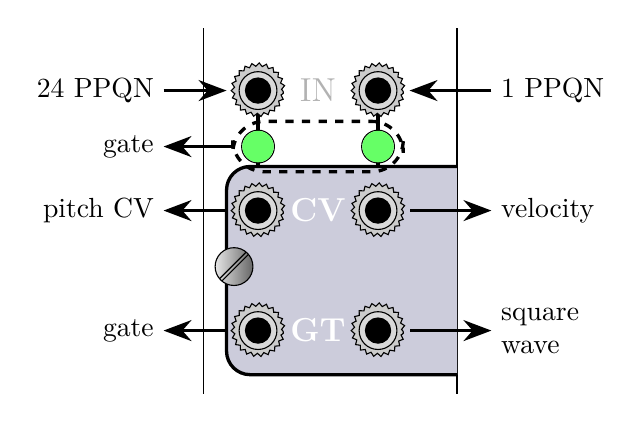
\begin{tikzpicture}[scale=0.8]
  {\setmainfont[Path={../../tsukurimashou/otf/},
BoldFont={TsukurimashouBokukkoExtraBoldPS}]{TsukurimashouBokukkoDemiboldPS}%
% start out defining coordinates
\coordinate (lbh) at (4.91mm,31.23mm) {};
\coordinate (j1) at (8.72mm,59.17mm) {};
\coordinate (j2) at (27.77mm,59.17mm) {};
\coordinate (j3) at (8.72mm,40.12mm) {};
\coordinate (j4) at (27.77mm,40.12mm) {};
\coordinate (j5) at (8.72mm,21.07mm) {};
\coordinate (j6) at (27.77mm,21.07mm) {};
\coordinate (d5) at (8.72mm,50.28mm) {};
\coordinate (d6) at (27.77mm,50.28mm) {};
%
\draw (0,11.07mm) -- (0,69.07mm);
\draw (40.30mm,11.07mm) -- (40.30mm,69.07mm);
%
\draw[very thick,black] (j1) -- (j3);
\draw[very thick,black] (j2) -- (j4);
\draw[very thick,black,fill=blue!30!black!20!white,rounded corners=3.0mm]
  (40.30mm,47.12mm) -- (3.72mm,47.12mm) --
  (3.72mm,14.07mm) -- (40.33mm,14.07mm);
\node[black!30!white] at ($(j1)!0.5!(j2)$) {\large IN};
\node[white] at ($(j3)!0.5!(j4)$) {\large\textbf{CV}};
\node[white] at ($(j5)!0.5!(j6)$) {\large\textbf{GT}};
%
% board-to-panel mounting holes, to clear M3 machine screw
\draw (lbh) circle[radius=1.60mm];
% six jacks with M6 threads, 6.3mm holes
\draw (j1) circle[radius=3.15mm];
\draw (j2) circle[radius=3.15mm];
\draw (j3) circle[radius=3.15mm];
\draw (j4) circle[radius=3.15mm];
\draw (j5) circle[radius=3.15mm];
\draw (j6) circle[radius=3.15mm];
% two LEDs, 5.20mm holes
\draw (d5) circle[radius=2.60mm];
\draw (d6) circle[radius=2.60mm];
%
% mock up screw heads, knobs
% machine screws with 6mm heads
\foreach \screwname in {lbh} {
  \path[draw=black,shading=ball,
    left color=black!10!white,right color=black!60!white]
    (\screwname) circle[radius=3mm];
  \draw ($(\screwname)+(50:3.0mm)$)--($(\screwname)+(220:3.0mm)$);
  \draw ($(\screwname)+(40:3.0mm)$)--($(\screwname)+(230:3.0mm)$);
}
% jacks with knurled nuts
\foreach \jackname in {j1,j2,j3,j4,j5,j6} {
  \path[draw=black,fill=black!20!white,
    decorate,decoration={snake,amplitude=0.6,segment length=2.5}]
    ($(\jackname)+(0,-0.15mm)$) circle[radius=4mm];
  \path[draw=black,fill=black!15!white] (\jackname) circle[radius=3mm];
  \path[draw=black,fill=black] (\jackname) circle[radius=2mm];
}
}

%
  \path[fill=green!60!white] (d5) circle[radius=2.50mm];
  \path[fill=green!60!white] (d6) circle[radius=2.50mm];
  \draw[very thick,-{Stealth[scale=1.2]}]
    ($(j1)+(-15mm,0)$) -- ($(j1)+(-5mm,0)$);
  \draw[very thick,-{Stealth[scale=1.2]}]
    ($(j2)+(18mm,0)$) -- ($(j2)+(5mm,0)$);
  \draw[very thick,{Stealth[scale=1.2]}-]
    ($(d5)+(-15mm,0)$) -- ($(d5)+(-4mm,0)$);
%  \draw[very thick,{Stealth[scale=1.2]}-]
%    ($(d6)+(18mm,0)$) -- ($(d6)+(4mm,0)$);
  \draw[rounded corners=4mm,very thick,dashed]
    ($(d5)+(-4mm,-4mm)$) rectangle ($(d6)+(4mm,4mm)$);
  \draw[very thick,{Stealth[scale=1.2]}-]
    ($(j3)+(-15mm,0)$) -- ($(j3)+(-5mm,0)$);
  \draw[very thick,{Stealth[scale=1.2]}-]
    ($(j4)+(18mm,0)$) -- ($(j4)+(5mm,0)$);
  \draw[very thick,{Stealth[scale=1.2]}-]
    ($(j5)+(-15mm,0)$) -- ($(j5)+(-5mm,0)$);
  \draw[very thick,{Stealth[scale=1.2]}-]
    ($(j6)+(18mm,0)$) -- ($(j6)+(5mm,0)$);
%
  \node[anchor=east] at ($(j1)+(-15mm,0)$) {24 PPQN};
  \node[anchor=west] at ($(j2)+(18mm,0)$) {1 PPQN};
  \node[anchor=east] at ($(d5)+(-15mm,0)$) {gate};
  \node[anchor=east] at ($(j3)+(-15mm,0)$) {pitch CV};
  \node[anchor=west] at ($(j4)+(18mm,0)$) {velocity};
  \node[anchor=east] at ($(j5)+(-15mm,0)$) {gate};
  \node[anchor=west] at ($(j6)+(18mm,0)$)
    {\parbox{12mm}{square wave}};
\end{tikzpicture}\par}

Channel 1 implements monophonic note stealing.  If a new note starts while
an old one is in progress, then the old note immediately ends and is
replaced by the new one.  In such a case the gate output goes low for
approximately 1ms to signal the start of the new note.

A stolen note ends when it is stolen.  For instance, if you play Note On C,
Note On G, Note Off G, then the gate goes low and the oscillator continues
playing G.  The C does not come back when the G ends, even if you still
have not yet played Note Off C.

Although in this mode the module does not \emph{use} its tempo clock, it can
\emph{accept} clock signals on the input jacks.  The left input jack accepts
a standard 24~PPQN MIDI clock.  The right input jack will function as a
1~PPQN or tap tempo input if there is nothing received on the left
input, or as a synchronization or reset input (marking the start of a
quarter note) when there is also a 24~PPQN clock being received on the left.

%%%%%%%%%%%%%%%%%%%%%%%%%%%%%%%%%%%%%%%%%%%%%%%%%%%%%%%%%%%%%%%%%%%%%%%%

\section{Channel 2:  duophonic CV/gate}

This mode is intended for controlling a synthesizer with two more or less
identical voices.  Each voice has a pitch CV and a gate CV, which respond to
Note On and Off messages for up to two simultaneous notes in the same MIDI
channel.

{\centering
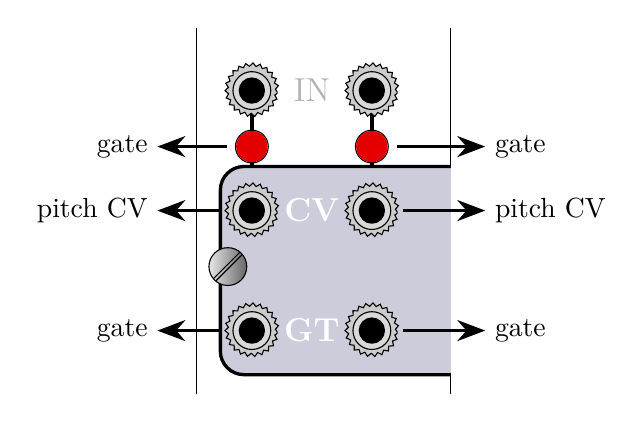
\begin{tikzpicture}[scale=0.8]
  {\setmainfont[Path={../../tsukurimashou/otf/},
BoldFont={TsukurimashouBokukkoExtraBoldPS}]{TsukurimashouBokukkoDemiboldPS}%
% start out defining coordinates
\coordinate (lbh) at (4.91mm,31.23mm) {};
\coordinate (j1) at (8.72mm,59.17mm) {};
\coordinate (j2) at (27.77mm,59.17mm) {};
\coordinate (j3) at (8.72mm,40.12mm) {};
\coordinate (j4) at (27.77mm,40.12mm) {};
\coordinate (j5) at (8.72mm,21.07mm) {};
\coordinate (j6) at (27.77mm,21.07mm) {};
\coordinate (d5) at (8.72mm,50.28mm) {};
\coordinate (d6) at (27.77mm,50.28mm) {};
%
\draw (0,11.07mm) -- (0,69.07mm);
\draw (40.30mm,11.07mm) -- (40.30mm,69.07mm);
%
\draw[very thick,black] (j1) -- (j3);
\draw[very thick,black] (j2) -- (j4);
\draw[very thick,black,fill=blue!30!black!20!white,rounded corners=3.0mm]
  (40.30mm,47.12mm) -- (3.72mm,47.12mm) --
  (3.72mm,14.07mm) -- (40.33mm,14.07mm);
\node[black!30!white] at ($(j1)!0.5!(j2)$) {\large IN};
\node[white] at ($(j3)!0.5!(j4)$) {\large\textbf{CV}};
\node[white] at ($(j5)!0.5!(j6)$) {\large\textbf{GT}};
%
% board-to-panel mounting holes, to clear M3 machine screw
\draw (lbh) circle[radius=1.60mm];
% six jacks with M6 threads, 6.3mm holes
\draw (j1) circle[radius=3.15mm];
\draw (j2) circle[radius=3.15mm];
\draw (j3) circle[radius=3.15mm];
\draw (j4) circle[radius=3.15mm];
\draw (j5) circle[radius=3.15mm];
\draw (j6) circle[radius=3.15mm];
% two LEDs, 5.20mm holes
\draw (d5) circle[radius=2.60mm];
\draw (d6) circle[radius=2.60mm];
%
% mock up screw heads, knobs
% machine screws with 6mm heads
\foreach \screwname in {lbh} {
  \path[draw=black,shading=ball,
    left color=black!10!white,right color=black!60!white]
    (\screwname) circle[radius=3mm];
  \draw ($(\screwname)+(50:3.0mm)$)--($(\screwname)+(220:3.0mm)$);
  \draw ($(\screwname)+(40:3.0mm)$)--($(\screwname)+(230:3.0mm)$);
}
% jacks with knurled nuts
\foreach \jackname in {j1,j2,j3,j4,j5,j6} {
  \path[draw=black,fill=black!20!white,
    decorate,decoration={snake,amplitude=0.6,segment length=2.5}]
    ($(\jackname)+(0,-0.15mm)$) circle[radius=4mm];
  \path[draw=black,fill=black!15!white] (\jackname) circle[radius=3mm];
  \path[draw=black,fill=black] (\jackname) circle[radius=2mm];
}
}

%
  \path[fill=red!90!black] (d5) circle[radius=2.50mm];
  \path[fill=red!90!black] (d6) circle[radius=2.50mm];
%  \draw[very thick,-{Stealth[scale=1.2]}]
%    ($(j1)+(-15mm,0)$) -- ($(j1)+(-5mm,0)$);
%  \draw[very thick,-{Stealth[scale=1.2]}]
%    ($(j2)+(18mm,0)$) -- ($(j2)+(5mm,0)$);
  \draw[very thick,{Stealth[scale=1.2]}-]
    ($(d5)+(-15mm,0)$) -- ($(d5)+(-4mm,0)$);
  \draw[very thick,{Stealth[scale=1.2]}-]
    ($(d6)+(18mm,0)$) -- ($(d6)+(4mm,0)$);
  \draw[very thick,{Stealth[scale=1.2]}-]
    ($(j3)+(-15mm,0)$) -- ($(j3)+(-5mm,0)$);
  \draw[very thick,{Stealth[scale=1.2]}-]
    ($(j4)+(18mm,0)$) -- ($(j4)+(5mm,0)$);
  \draw[very thick,{Stealth[scale=1.2]}-]
    ($(j5)+(-15mm,0)$) -- ($(j5)+(-5mm,0)$);
  \draw[very thick,{Stealth[scale=1.2]}-]
    ($(j6)+(18mm,0)$) -- ($(j6)+(5mm,0)$);
%
  \node[anchor=east] at ($(d5)+(-15mm,0)$) {gate};
  \node[anchor=west] at ($(d6)+(18mm,0)$) {gate};
  \node[anchor=east] at ($(j3)+(-15mm,0)$) {pitch CV};
  \node[anchor=west] at ($(j4)+(18mm,0)$) {pitch CV};
  \node[anchor=east] at ($(j5)+(-15mm,0)$) {gate};
  \node[anchor=west] at ($(j6)+(18mm,0)$) {gate};
\end{tikzpicture}\par}

Channel~2 implements note stealing according to these rules:
\begin{itemize}
\item The first note goes to the left.
\item If exactly one side is free, a new note goes there.
\item Otherwise (both sides free, or neither), a new note goes to the side
that least recently had a new note.
\end{itemize}

As with Channel~1, the gate CV drops for about 1ms when a new note replaces
an old one, so as to give some chance of retriggering whatever module is
using that gate signal.  Also as in Channel~1, stolen notes end when they
are stolen.

Signals on the input jacks are ignored in this mode, and the LED on each
side glows red when there is a note active on the side in question.  Pitch
bend in this channel affects both sides.

%%%%%%%%%%%%%%%%%%%%%%%%%%%%%%%%%%%%%%%%%%%%%%%%%%%%%%%%%%%%%%%%%%%%%%%%

\section{Channels 3 and 4:  quantize to MIDI}

When it receives MIDI notes in either of these two channels, the Gracious
Host acts as a dual quantizer.  The input voltage on each side is compared
to whichever MIDI notes are currently held, and the output pitch control
voltages are set to the voltages for the notes closest to the inputs.

{\centering
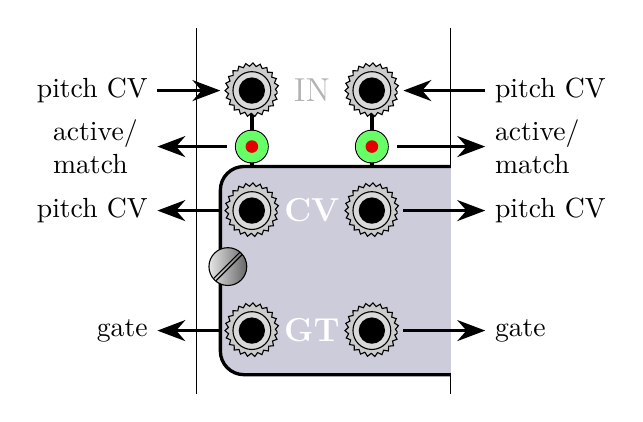
\begin{tikzpicture}[scale=0.8]
  {\setmainfont[Path={../../tsukurimashou/otf/},
BoldFont={TsukurimashouBokukkoExtraBoldPS}]{TsukurimashouBokukkoDemiboldPS}%
% start out defining coordinates
\coordinate (lbh) at (4.91mm,31.23mm) {};
\coordinate (j1) at (8.72mm,59.17mm) {};
\coordinate (j2) at (27.77mm,59.17mm) {};
\coordinate (j3) at (8.72mm,40.12mm) {};
\coordinate (j4) at (27.77mm,40.12mm) {};
\coordinate (j5) at (8.72mm,21.07mm) {};
\coordinate (j6) at (27.77mm,21.07mm) {};
\coordinate (d5) at (8.72mm,50.28mm) {};
\coordinate (d6) at (27.77mm,50.28mm) {};
%
\draw (0,11.07mm) -- (0,69.07mm);
\draw (40.30mm,11.07mm) -- (40.30mm,69.07mm);
%
\draw[very thick,black] (j1) -- (j3);
\draw[very thick,black] (j2) -- (j4);
\draw[very thick,black,fill=blue!30!black!20!white,rounded corners=3.0mm]
  (40.30mm,47.12mm) -- (3.72mm,47.12mm) --
  (3.72mm,14.07mm) -- (40.33mm,14.07mm);
\node[black!30!white] at ($(j1)!0.5!(j2)$) {\large IN};
\node[white] at ($(j3)!0.5!(j4)$) {\large\textbf{CV}};
\node[white] at ($(j5)!0.5!(j6)$) {\large\textbf{GT}};
%
% board-to-panel mounting holes, to clear M3 machine screw
\draw (lbh) circle[radius=1.60mm];
% six jacks with M6 threads, 6.3mm holes
\draw (j1) circle[radius=3.15mm];
\draw (j2) circle[radius=3.15mm];
\draw (j3) circle[radius=3.15mm];
\draw (j4) circle[radius=3.15mm];
\draw (j5) circle[radius=3.15mm];
\draw (j6) circle[radius=3.15mm];
% two LEDs, 5.20mm holes
\draw (d5) circle[radius=2.60mm];
\draw (d6) circle[radius=2.60mm];
%
% mock up screw heads, knobs
% machine screws with 6mm heads
\foreach \screwname in {lbh} {
  \path[draw=black,shading=ball,
    left color=black!10!white,right color=black!60!white]
    (\screwname) circle[radius=3mm];
  \draw ($(\screwname)+(50:3.0mm)$)--($(\screwname)+(220:3.0mm)$);
  \draw ($(\screwname)+(40:3.0mm)$)--($(\screwname)+(230:3.0mm)$);
}
% jacks with knurled nuts
\foreach \jackname in {j1,j2,j3,j4,j5,j6} {
  \path[draw=black,fill=black!20!white,
    decorate,decoration={snake,amplitude=0.6,segment length=2.5}]
    ($(\jackname)+(0,-0.15mm)$) circle[radius=4mm];
  \path[draw=black,fill=black!15!white] (\jackname) circle[radius=3mm];
  \path[draw=black,fill=black] (\jackname) circle[radius=2mm];
}
}

%
  \path[fill=green!60!white] (d5) circle[radius=2.50mm];
  \path[fill=green!60!white] (d6) circle[radius=2.50mm];
  \path[fill=red!90!black] (d5) circle[radius=1.0mm];
  \path[fill=red!90!black] (d6) circle[radius=1.0mm];
  \draw[very thick,-{Stealth[scale=1.2]}]
    ($(j1)+(-15mm,0)$) -- ($(j1)+(-5mm,0)$);
  \draw[very thick,-{Stealth[scale=1.2]}]
    ($(j2)+(18mm,0)$) -- ($(j2)+(5mm,0)$);
  \draw[very thick,{Stealth[scale=1.2]}-]
    ($(d5)+(-15mm,0)$) -- ($(d5)+(-4mm,0)$);
  \draw[very thick,{Stealth[scale=1.2]}-]
    ($(d6)+(18mm,0)$) -- ($(d6)+(4mm,0)$);
  \draw[very thick,{Stealth[scale=1.2]}-]
    ($(j3)+(-15mm,0)$) -- ($(j3)+(-5mm,0)$);
  \draw[very thick,{Stealth[scale=1.2]}-]
    ($(j4)+(18mm,0)$) -- ($(j4)+(5mm,0)$);
  \draw[very thick,{Stealth[scale=1.2]}-]
    ($(j5)+(-15mm,0)$) -- ($(j5)+(-5mm,0)$);
  \draw[very thick,{Stealth[scale=1.2]}-]
    ($(j6)+(18mm,0)$) -- ($(j6)+(5mm,0)$);
%
  \node[anchor=east] at ($(j1)+(-15mm,0)$) {pitch CV};
  \node[anchor=west] at ($(j2)+(18mm,0)$) {pitch CV};
  \node[anchor=east] at ($(d5)+(-15mm,0)$)
    {\parbox{12mm}{active/ match}};
  \node[anchor=west] at ($(d6)+(18mm,0)$)
    {\parbox{12mm}{active/ match}};
  \node[anchor=east] at ($(j3)+(-15mm,0)$) {pitch CV};
  \node[anchor=west] at ($(j4)+(18mm,0)$) {pitch CV};
  \node[anchor=east] at ($(j5)+(-15mm,0)$) {gate};
  \node[anchor=west] at ($(j6)+(18mm,0)$) {gate};
\end{tikzpicture}\par}

If, once in this mode, there happen to be no MIDI notes held, then all four
output voltages go to zero and the LEDs go dark.  Otherwise, the LED on each
side is red when the input happens to hit a quantized output value exactly
(that is, within the same semitone), and green otherwise.  Each gate output
is normally high when any notes are held, but it drops low for approximately
1ms when the associated pitch output goes to a new note, in order to allow
for retriggering of a synthesizer voice.

The difference between the two channels is that with Channel~3, quantization
is just to the received MIDI notes and no others.  With Channel~4, each
MIDI note counts as if you played it \emph{in every octave}.  So if you
play MIDI notes 60 and 69 (Middle C and the A above it, equivalent to output
voltages 2.00V and 2.75V) in Channel~3, then an input voltage of 0.50V
(equivalent to MIDI note 42) will quantize to 2.00V (MIDI note 60); but with
the same notes played in Channel~4, an input voltage of 0.50V will quantize
to 0.75V (MIDI note 45) because playing any C and A activates every C and A
as a possible quantization value.

Pitch bend, if nonzero, is applied to both outputs equally after
quantization; it does not affect the input quantization boundaries.  Some
future version of the firmware may attempt to do something more intelligent
with pitch bend, such as using it to support microtonal quantization.

%%%%%%%%%%%%%%%%%%%%%%%%%%%%%%%%%%%%%%%%%%%%%%%%%%%%%%%%%%%%%%%%%%%%%%%%

\section{Channels 5--7:  arpeggiator modes}

MIDI notes on these three channels will be arpeggiated to the CV and gate
outputs, in different styles depending on the channel.

{\centering
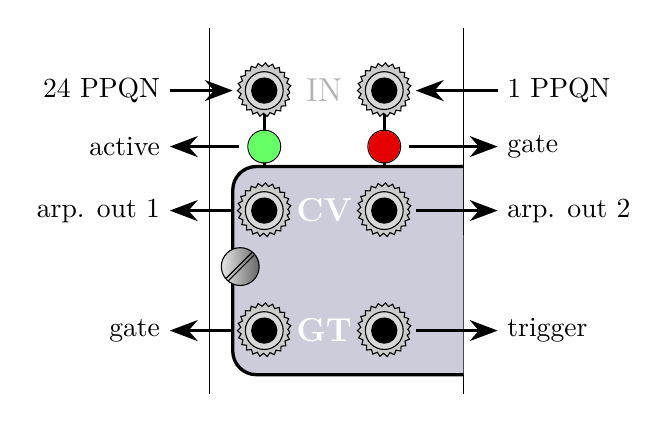
\begin{tikzpicture}[scale=0.8]
  {\setmainfont[Path={../../tsukurimashou/otf/},
BoldFont={TsukurimashouBokukkoExtraBoldPS}]{TsukurimashouBokukkoDemiboldPS}%
% start out defining coordinates
\coordinate (lbh) at (4.91mm,31.23mm) {};
\coordinate (j1) at (8.72mm,59.17mm) {};
\coordinate (j2) at (27.77mm,59.17mm) {};
\coordinate (j3) at (8.72mm,40.12mm) {};
\coordinate (j4) at (27.77mm,40.12mm) {};
\coordinate (j5) at (8.72mm,21.07mm) {};
\coordinate (j6) at (27.77mm,21.07mm) {};
\coordinate (d5) at (8.72mm,50.28mm) {};
\coordinate (d6) at (27.77mm,50.28mm) {};
%
\draw (0,11.07mm) -- (0,69.07mm);
\draw (40.30mm,11.07mm) -- (40.30mm,69.07mm);
%
\draw[very thick,black] (j1) -- (j3);
\draw[very thick,black] (j2) -- (j4);
\draw[very thick,black,fill=blue!30!black!20!white,rounded corners=3.0mm]
  (40.30mm,47.12mm) -- (3.72mm,47.12mm) --
  (3.72mm,14.07mm) -- (40.33mm,14.07mm);
\node[black!30!white] at ($(j1)!0.5!(j2)$) {\large IN};
\node[white] at ($(j3)!0.5!(j4)$) {\large\textbf{CV}};
\node[white] at ($(j5)!0.5!(j6)$) {\large\textbf{GT}};
%
% board-to-panel mounting holes, to clear M3 machine screw
\draw (lbh) circle[radius=1.60mm];
% six jacks with M6 threads, 6.3mm holes
\draw (j1) circle[radius=3.15mm];
\draw (j2) circle[radius=3.15mm];
\draw (j3) circle[radius=3.15mm];
\draw (j4) circle[radius=3.15mm];
\draw (j5) circle[radius=3.15mm];
\draw (j6) circle[radius=3.15mm];
% two LEDs, 5.20mm holes
\draw (d5) circle[radius=2.60mm];
\draw (d6) circle[radius=2.60mm];
%
% mock up screw heads, knobs
% machine screws with 6mm heads
\foreach \screwname in {lbh} {
  \path[draw=black,shading=ball,
    left color=black!10!white,right color=black!60!white]
    (\screwname) circle[radius=3mm];
  \draw ($(\screwname)+(50:3.0mm)$)--($(\screwname)+(220:3.0mm)$);
  \draw ($(\screwname)+(40:3.0mm)$)--($(\screwname)+(230:3.0mm)$);
}
% jacks with knurled nuts
\foreach \jackname in {j1,j2,j3,j4,j5,j6} {
  \path[draw=black,fill=black!20!white,
    decorate,decoration={snake,amplitude=0.6,segment length=2.5}]
    ($(\jackname)+(0,-0.15mm)$) circle[radius=4mm];
  \path[draw=black,fill=black!15!white] (\jackname) circle[radius=3mm];
  \path[draw=black,fill=black] (\jackname) circle[radius=2mm];
}
}

%
  \path[fill=green!60!white] (d5) circle[radius=2.50mm];
  \path[fill=red!90!black] (d6) circle[radius=2.50mm];
  \draw[very thick,-{Stealth[scale=1.2]}]
    ($(j1)+(-15mm,0)$) -- ($(j1)+(-5mm,0)$);
  \draw[very thick,-{Stealth[scale=1.2]}]
    ($(j2)+(18mm,0)$) -- ($(j2)+(5mm,0)$);
  \draw[very thick,{Stealth[scale=1.2]}-]
    ($(d5)+(-15mm,0)$) -- ($(d5)+(-4mm,0)$);
  \draw[very thick,{Stealth[scale=1.2]}-]
    ($(d6)+(18mm,0)$) -- ($(d6)+(4mm,0)$);
  \draw[very thick,{Stealth[scale=1.2]}-]
    ($(j3)+(-15mm,0)$) -- ($(j3)+(-5mm,0)$);
  \draw[very thick,{Stealth[scale=1.2]}-]
    ($(j4)+(18mm,0)$) -- ($(j4)+(5mm,0)$);
  \draw[very thick,{Stealth[scale=1.2]}-]
    ($(j5)+(-15mm,0)$) -- ($(j5)+(-5mm,0)$);
  \draw[very thick,{Stealth[scale=1.2]}-]
    ($(j6)+(18mm,0)$) -- ($(j6)+(5mm,0)$);
%
  \node[anchor=east] at ($(j1)+(-15mm,0)$) {24 PPQN};
  \node[anchor=west] at ($(j2)+(18mm,0)$) {1 PPQN};
  \node[anchor=east] at ($(d5)+(-15mm,0)$) {active};
  \node[anchor=west] at ($(d6)+(18mm,0)$) {gate};
  \node[anchor=east] at ($(j3)+(-15mm,0)$) {arp. out 1};
  \node[anchor=west] at ($(j4)+(18mm,0)$) {arp. out 2};
  \node[anchor=east] at ($(j5)+(-15mm,0)$) {gate};
  \node[anchor=west] at ($(j6)+(18mm,0)$) {trigger};
\end{tikzpicture}\par}

These channels use the global MIDI clock.  MIDI Timing Clock messages, or
pulses received on the left input jack, define the tempo at a rate of
24~PPQN.  MIDI Start messages reset to the start of the quarter note. 
Pulses received on the right input jack, and the tap tempo key on a typing
keyboard, reset to the start of the quarter note and also define the tempo
when there is no 24~PPQN clock.

The left digital output is the gate; it goes high (9V nominal) and the right
LED glows red, for the first 7/8 of each quarter note time.  The right
digital output produces a 960$\mu$s trigger at the start of each quarter
note time; this can also function as a 1~PPQN clock for other modules.  The
left LED glows green when there are any held notes, that is, when the
arpeggiator is active.  As for the CV outputs, they cycle through the held
MIDI notes in a way that depends on the channel.

Channel~5 arpeggiates up and down.  The left output cycles through the notes
upward (in order of increasing pitch) while the right output cycles
downward.

Channel~6 arpeggiates the held notes in the order they were entered, with
the right output one step ahead of the left.

Channel~7 arpeggiates in random order.  In more detail, the right output
selects one of the held notes uniformly at random on each beat.  That means
\emph{every} held note is available; the right output can repeat notes.  The
left output selects a note at random, but if there are at least two held
notes then it will avoid choosing the same note as the right output, and if
there are at least three held notes then it will also avoid its own previous
value; other than those exceptions, it selects uniformly.  So the left
output will not repeat notes, given sufficient held notes to choose from. 
The random numbers for Channel~7 come from a hashed entropy pool
continuously reseeded by I/O timings, and they should be random enough for
rock'n'roll even if not cryptographically certifiable.

All three arpeggiation modes start their new notes \emph{on the beat}.  If
you start playing notes into these channels when the tempo is slow, there
may be a noticeable delay before the output starts playing; but this design
feature is intended to allow playing more precisely \emph{with} the beat in
typical modular performance styles.  Note that the tempo clock needs to be
running in order for the arpeggiator to be useful.  To use these channels
you must provide the module with MIDI clock messages, a clock on the input
jacks, or tap tempo from a typing keyboard.

%%%%%%%%%%%%%%%%%%%%%%%%%%%%%%%%%%%%%%%%%%%%%%%%%%%%%%%%%%%%%%%%%%%%%%%%

\section{Channels 8 and 9:  dual mono}

These two channels work together to allow independent control of two GV/gate
synthesizer voices.  Unlike Channel~2, which automatically assigns incoming
notes to either channel, you can use this pair of channels to specify on
which side each note will play.  Channel~8 controls the left and Channel~9
the right.

{\centering
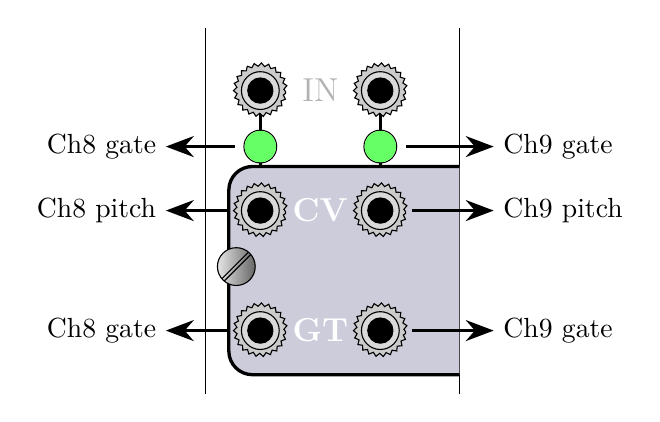
\begin{tikzpicture}[scale=0.8]
  {\setmainfont[Path={../../tsukurimashou/otf/},
BoldFont={TsukurimashouBokukkoExtraBoldPS}]{TsukurimashouBokukkoDemiboldPS}%
% start out defining coordinates
\coordinate (lbh) at (4.91mm,31.23mm) {};
\coordinate (j1) at (8.72mm,59.17mm) {};
\coordinate (j2) at (27.77mm,59.17mm) {};
\coordinate (j3) at (8.72mm,40.12mm) {};
\coordinate (j4) at (27.77mm,40.12mm) {};
\coordinate (j5) at (8.72mm,21.07mm) {};
\coordinate (j6) at (27.77mm,21.07mm) {};
\coordinate (d5) at (8.72mm,50.28mm) {};
\coordinate (d6) at (27.77mm,50.28mm) {};
%
\draw (0,11.07mm) -- (0,69.07mm);
\draw (40.30mm,11.07mm) -- (40.30mm,69.07mm);
%
\draw[very thick,black] (j1) -- (j3);
\draw[very thick,black] (j2) -- (j4);
\draw[very thick,black,fill=blue!30!black!20!white,rounded corners=3.0mm]
  (40.30mm,47.12mm) -- (3.72mm,47.12mm) --
  (3.72mm,14.07mm) -- (40.33mm,14.07mm);
\node[black!30!white] at ($(j1)!0.5!(j2)$) {\large IN};
\node[white] at ($(j3)!0.5!(j4)$) {\large\textbf{CV}};
\node[white] at ($(j5)!0.5!(j6)$) {\large\textbf{GT}};
%
% board-to-panel mounting holes, to clear M3 machine screw
\draw (lbh) circle[radius=1.60mm];
% six jacks with M6 threads, 6.3mm holes
\draw (j1) circle[radius=3.15mm];
\draw (j2) circle[radius=3.15mm];
\draw (j3) circle[radius=3.15mm];
\draw (j4) circle[radius=3.15mm];
\draw (j5) circle[radius=3.15mm];
\draw (j6) circle[radius=3.15mm];
% two LEDs, 5.20mm holes
\draw (d5) circle[radius=2.60mm];
\draw (d6) circle[radius=2.60mm];
%
% mock up screw heads, knobs
% machine screws with 6mm heads
\foreach \screwname in {lbh} {
  \path[draw=black,shading=ball,
    left color=black!10!white,right color=black!60!white]
    (\screwname) circle[radius=3mm];
  \draw ($(\screwname)+(50:3.0mm)$)--($(\screwname)+(220:3.0mm)$);
  \draw ($(\screwname)+(40:3.0mm)$)--($(\screwname)+(230:3.0mm)$);
}
% jacks with knurled nuts
\foreach \jackname in {j1,j2,j3,j4,j5,j6} {
  \path[draw=black,fill=black!20!white,
    decorate,decoration={snake,amplitude=0.6,segment length=2.5}]
    ($(\jackname)+(0,-0.15mm)$) circle[radius=4mm];
  \path[draw=black,fill=black!15!white] (\jackname) circle[radius=3mm];
  \path[draw=black,fill=black] (\jackname) circle[radius=2mm];
}
}

%
  \path[fill=green!60!white] (d5) circle[radius=2.50mm];
  \path[fill=green!60!white] (d6) circle[radius=2.50mm];
  \draw[very thick,{Stealth[scale=1.2]}-]
    ($(d5)+(-15mm,0)$) -- ($(d5)+(-4mm,0)$);
  \draw[very thick,{Stealth[scale=1.2]}-]
    ($(d6)+(18mm,0)$) -- ($(d6)+(4mm,0)$);
  \draw[very thick,{Stealth[scale=1.2]}-]
    ($(j3)+(-15mm,0)$) -- ($(j3)+(-5mm,0)$);
  \draw[very thick,{Stealth[scale=1.2]}-]
    ($(j4)+(18mm,0)$) -- ($(j4)+(5mm,0)$);
  \draw[very thick,{Stealth[scale=1.2]}-]
    ($(j5)+(-15mm,0)$) -- ($(j5)+(-5mm,0)$);
  \draw[very thick,{Stealth[scale=1.2]}-]
    ($(j6)+(18mm,0)$) -- ($(j6)+(5mm,0)$);
%
  \node[anchor=east] at ($(d5)+(-15mm,0)$) {Ch8 gate};
  \node[anchor=west] at ($(d6)+(18mm,0)$) {Ch9 gate};
  \node[anchor=east] at ($(j3)+(-15mm,0)$) {Ch8 pitch};
  \node[anchor=west] at ($(j4)+(18mm,0)$) {Ch9 pitch};
  \node[anchor=east] at ($(j5)+(-15mm,0)$) {Ch8 gate};
  \node[anchor=west] at ($(j6)+(18mm,0)$) {Ch9 gate};
\end{tikzpicture}\par}

Much like Channel~1, these channels do monophonic note stealing.  The
LED for each channel glows green when a note is playing.  The input jacks
are ignored.  Channels~8 and~9 have independent pitch bend.

%%%%%%%%%%%%%%%%%%%%%%%%%%%%%%%%%%%%%%%%%%%%%%%%%%%%%%%%%%%%%%%%%%%%%%%%

\section{Channels 10 and 11:  drum notes}

These channels map note numbers into pulses on the four output jacks. 
Channel~10 produces a trigger of approximately 1ms at the start of each
note, whereas Channel~11 produces a gate pulse, high as long as the note
lasts.

Note numbers translate to output jacks according to a somewhat complicated
mapping that is designed to work without needing special configuration on
many common MIDI controllers.  As a simple starting point, this
assignment of General MIDI drum notes to output jacks is one that works:
\begin{itemize}
\item MIDI note 36 (Bass Drum 1): lower right
\item MIDI note 38 (Acoustic Snare): upper left
\item MIDI note 40 (Electric Snare): upper right
\item MIDI note 42 (Closed Hi Hat): lower left
\end{itemize}

{\centering
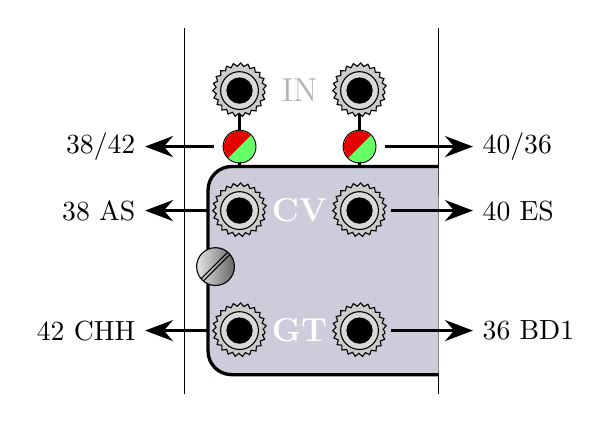
\begin{tikzpicture}[scale=0.8]
  {\setmainfont[Path={../../tsukurimashou/otf/},
BoldFont={TsukurimashouBokukkoExtraBoldPS}]{TsukurimashouBokukkoDemiboldPS}%
% start out defining coordinates
\coordinate (lbh) at (4.91mm,31.23mm) {};
\coordinate (j1) at (8.72mm,59.17mm) {};
\coordinate (j2) at (27.77mm,59.17mm) {};
\coordinate (j3) at (8.72mm,40.12mm) {};
\coordinate (j4) at (27.77mm,40.12mm) {};
\coordinate (j5) at (8.72mm,21.07mm) {};
\coordinate (j6) at (27.77mm,21.07mm) {};
\coordinate (d5) at (8.72mm,50.28mm) {};
\coordinate (d6) at (27.77mm,50.28mm) {};
%
\draw (0,11.07mm) -- (0,69.07mm);
\draw (40.30mm,11.07mm) -- (40.30mm,69.07mm);
%
\draw[very thick,black] (j1) -- (j3);
\draw[very thick,black] (j2) -- (j4);
\draw[very thick,black,fill=blue!30!black!20!white,rounded corners=3.0mm]
  (40.30mm,47.12mm) -- (3.72mm,47.12mm) --
  (3.72mm,14.07mm) -- (40.33mm,14.07mm);
\node[black!30!white] at ($(j1)!0.5!(j2)$) {\large IN};
\node[white] at ($(j3)!0.5!(j4)$) {\large\textbf{CV}};
\node[white] at ($(j5)!0.5!(j6)$) {\large\textbf{GT}};
%
% board-to-panel mounting holes, to clear M3 machine screw
\draw (lbh) circle[radius=1.60mm];
% six jacks with M6 threads, 6.3mm holes
\draw (j1) circle[radius=3.15mm];
\draw (j2) circle[radius=3.15mm];
\draw (j3) circle[radius=3.15mm];
\draw (j4) circle[radius=3.15mm];
\draw (j5) circle[radius=3.15mm];
\draw (j6) circle[radius=3.15mm];
% two LEDs, 5.20mm holes
\draw (d5) circle[radius=2.60mm];
\draw (d6) circle[radius=2.60mm];
%
% mock up screw heads, knobs
% machine screws with 6mm heads
\foreach \screwname in {lbh} {
  \path[draw=black,shading=ball,
    left color=black!10!white,right color=black!60!white]
    (\screwname) circle[radius=3mm];
  \draw ($(\screwname)+(50:3.0mm)$)--($(\screwname)+(220:3.0mm)$);
  \draw ($(\screwname)+(40:3.0mm)$)--($(\screwname)+(230:3.0mm)$);
}
% jacks with knurled nuts
\foreach \jackname in {j1,j2,j3,j4,j5,j6} {
  \path[draw=black,fill=black!20!white,
    decorate,decoration={snake,amplitude=0.6,segment length=2.5}]
    ($(\jackname)+(0,-0.15mm)$) circle[radius=4mm];
  \path[draw=black,fill=black!15!white] (\jackname) circle[radius=3mm];
  \path[draw=black,fill=black] (\jackname) circle[radius=2mm];
}
}

%
  \path[fill=green!60!white] (d5) circle[radius=2.50mm];
  \path[fill=red!90!black] ($(d5)+(225:2.5mm)$)
    arc[start angle=225,end angle=45,radius=2.50mm] --cycle;
  \path[fill=green!60!white] (d6) circle[radius=2.50mm];
  \path[fill=red!90!black] ($(d6)+(225:2.5mm)$)
    arc[start angle=225,end angle=45,radius=2.50mm] --cycle;
  \draw[very thick,{Stealth[scale=1.2]}-]
    ($(d5)+(-15mm,0)$) -- ($(d5)+(-4mm,0)$);
  \draw[very thick,{Stealth[scale=1.2]}-]
    ($(d6)+(18mm,0)$) -- ($(d6)+(4mm,0)$);
  \draw[very thick,{Stealth[scale=1.2]}-]
    ($(j3)+(-15mm,0)$) -- ($(j3)+(-5mm,0)$);
  \draw[very thick,{Stealth[scale=1.2]}-]
    ($(j4)+(18mm,0)$) -- ($(j4)+(5mm,0)$);
  \draw[very thick,{Stealth[scale=1.2]}-]
    ($(j5)+(-15mm,0)$) -- ($(j5)+(-5mm,0)$);
  \draw[very thick,{Stealth[scale=1.2]}-]
    ($(j6)+(18mm,0)$) -- ($(j6)+(5mm,0)$);
%
  \node[anchor=east] at ($(d5)+(-15mm,0)$) {38/42};
  \node[anchor=west] at ($(d6)+(18mm,0)$) {40/36};
  \node[anchor=east] at ($(j3)+(-15mm,0)$) {38 AS};
  \node[anchor=west] at ($(j4)+(18mm,0)$) {40 ES};
  \node[anchor=east] at ($(j5)+(-15mm,0)$) {42 CHH};
  \node[anchor=west] at ($(j6)+(18mm,0)$) {36 BD1};
\end{tikzpicture}\par}

Signals on the input jacks are ignored.  Each LED glows if any notes on
the corresponding side are active, red if the upper note (analog CV
output) is active and green if the lower but not the upper note is
active.

The upper analog outputs in drum mode go to their maximum voltage when high,
which is 5.5V nominal (uncalibrated).  The lower digital outputs, as usual,
go to about 9V.  The trigger pulse width is nominally 960$\mu$s.

Now, some more detail on how note mapping works.  Every MIDI note maps to one
of the four output jacks, so you can make up a mapping by choosing any four
notes that happen to map to different jacks.  If you have a controller like
a keyboard with many notes on it, you can probably find a usable mapping
quickly just through trial and error, but the scheme is designed to
guarantee that:
\begin{itemize}
\item any four consecutive MIDI notes starting with a multiple of four, such
as $\{0,1,2,3\}$ or $\{60,61,62,63\}$, will map to distinct jacks; and
\item any four MIDI notes spaced two apart, such as $\{0,2,4,6\}$ or
$\{65,67,69,71\}$, will map to distinct jacks.
\end{itemize}

That means pad controllers which typically assign the pads to consecutive
notes will often have four conveniently-arranged pads which control the four
output jacks.  It also means that the notes F, G, A, B (which are two
semitones apart) in any octave on a piano-style keyboard, or any four
horizontally adjacent keys on a Wicki-Hayden isomorphic keyboard (as
discussed in the typing-keyboard chapter of this manual), will work.

In even more detail:  each note number $N$ maps to a jack number $j=(\lfloor
N/4 \rfloor+N) \bmod 4$.  In words, that formula says to start with the note
number $N$, divide it by four and throw away the remainder, then add the
original $N$, divide the result by four again, and this time throw away the
quotient and look at only the remainder, which we'll call $j$.  Then:
\begin{itemize}
\item if $j=0$, the note activates the lower left jack;
\item if $j=1$, it activates the lower right jack;
\item if $j=2$, the upper left jack; and
\item if $j=3$, the upper right.
\end{itemize}

That splits the range of MIDI note numbers into four sets with the desired
properties of being hit by many convenient controller assignments.

{\centering
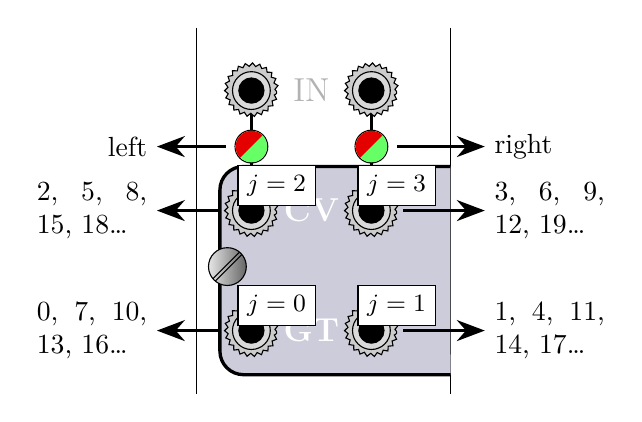
\begin{tikzpicture}[scale=0.8]
  {\setmainfont[Path={../../tsukurimashou/otf/},
BoldFont={TsukurimashouBokukkoExtraBoldPS}]{TsukurimashouBokukkoDemiboldPS}%
% start out defining coordinates
\coordinate (lbh) at (4.91mm,31.23mm) {};
\coordinate (j1) at (8.72mm,59.17mm) {};
\coordinate (j2) at (27.77mm,59.17mm) {};
\coordinate (j3) at (8.72mm,40.12mm) {};
\coordinate (j4) at (27.77mm,40.12mm) {};
\coordinate (j5) at (8.72mm,21.07mm) {};
\coordinate (j6) at (27.77mm,21.07mm) {};
\coordinate (d5) at (8.72mm,50.28mm) {};
\coordinate (d6) at (27.77mm,50.28mm) {};
%
\draw (0,11.07mm) -- (0,69.07mm);
\draw (40.30mm,11.07mm) -- (40.30mm,69.07mm);
%
\draw[very thick,black] (j1) -- (j3);
\draw[very thick,black] (j2) -- (j4);
\draw[very thick,black,fill=blue!30!black!20!white,rounded corners=3.0mm]
  (40.30mm,47.12mm) -- (3.72mm,47.12mm) --
  (3.72mm,14.07mm) -- (40.33mm,14.07mm);
\node[black!30!white] at ($(j1)!0.5!(j2)$) {\large IN};
\node[white] at ($(j3)!0.5!(j4)$) {\large\textbf{CV}};
\node[white] at ($(j5)!0.5!(j6)$) {\large\textbf{GT}};
%
% board-to-panel mounting holes, to clear M3 machine screw
\draw (lbh) circle[radius=1.60mm];
% six jacks with M6 threads, 6.3mm holes
\draw (j1) circle[radius=3.15mm];
\draw (j2) circle[radius=3.15mm];
\draw (j3) circle[radius=3.15mm];
\draw (j4) circle[radius=3.15mm];
\draw (j5) circle[radius=3.15mm];
\draw (j6) circle[radius=3.15mm];
% two LEDs, 5.20mm holes
\draw (d5) circle[radius=2.60mm];
\draw (d6) circle[radius=2.60mm];
%
% mock up screw heads, knobs
% machine screws with 6mm heads
\foreach \screwname in {lbh} {
  \path[draw=black,shading=ball,
    left color=black!10!white,right color=black!60!white]
    (\screwname) circle[radius=3mm];
  \draw ($(\screwname)+(50:3.0mm)$)--($(\screwname)+(220:3.0mm)$);
  \draw ($(\screwname)+(40:3.0mm)$)--($(\screwname)+(230:3.0mm)$);
}
% jacks with knurled nuts
\foreach \jackname in {j1,j2,j3,j4,j5,j6} {
  \path[draw=black,fill=black!20!white,
    decorate,decoration={snake,amplitude=0.6,segment length=2.5}]
    ($(\jackname)+(0,-0.15mm)$) circle[radius=4mm];
  \path[draw=black,fill=black!15!white] (\jackname) circle[radius=3mm];
  \path[draw=black,fill=black] (\jackname) circle[radius=2mm];
}
}

%
  \path[fill=green!60!white] (d5) circle[radius=2.50mm];
  \path[fill=red!90!black] ($(d5)+(225:2.5mm)$)
    arc[start angle=225,end angle=45,radius=2.50mm] --cycle;
  \path[fill=green!60!white] (d6) circle[radius=2.50mm];
  \path[fill=red!90!black] ($(d6)+(225:2.5mm)$)
    arc[start angle=225,end angle=45,radius=2.50mm] --cycle;
  \draw[very thick,{Stealth[scale=1.2]}-]
    ($(d5)+(-15mm,0)$) -- ($(d5)+(-4mm,0)$);
  \draw[very thick,{Stealth[scale=1.2]}-]
    ($(d6)+(18mm,0)$) -- ($(d6)+(4mm,0)$);
  \draw[very thick,{Stealth[scale=1.2]}-]
    ($(j3)+(-15mm,0)$) -- ($(j3)+(-5mm,0)$);
  \draw[very thick,{Stealth[scale=1.2]}-]
    ($(j4)+(18mm,0)$) -- ($(j4)+(5mm,0)$);
  \draw[very thick,{Stealth[scale=1.2]}-]
    ($(j5)+(-15mm,0)$) -- ($(j5)+(-5mm,0)$);
  \draw[very thick,{Stealth[scale=1.2]}-]
    ($(j6)+(18mm,0)$) -- ($(j6)+(5mm,0)$);
%
  \node[anchor=east] at ($(d5)+(-15mm,0)$) {left};
  \node[anchor=west] at ($(d6)+(18mm,0)$) {right};
  \node[anchor=east] at ($(j3)+(-15mm,0)$)
    {\parbox{14mm}{2, 5, 8, 15, 18\ldots}};
  \node[anchor=west] at ($(j4)+(18mm,0)$)
    {\parbox{14mm}{3, 6, 9, 12, 19\ldots}};
  \node[anchor=east] at ($(j5)+(-15mm,0)$)
    {\parbox{14mm}{0, 7, 10, 13, 16\ldots}};
  \node[anchor=west] at ($(j6)+(18mm,0)$)
    {\parbox{14mm}{1, 4, 11, 14, 17\ldots}};
  \node[draw,fill=white] at ($(j5)+(4mm,4mm)$) {\small $j=0$};
  \node[draw,fill=white] at ($(j6)+(4mm,4mm)$) {\small $j=1$};
  \node[draw,fill=white] at ($(j3)+(4mm,4mm)$) {\small $j=2$};
  \node[draw,fill=white] at ($(j4)+(4mm,4mm)$) {\small $j=3$};
\end{tikzpicture}\par}

%%%%%%%%%%%%%%%%%%%%%%%%%%%%%%%%%%%%%%%%%%%%%%%%%%%%%%%%%%%%%%%%%%%%%%%%

\section{Channel 12:  mono with clock out}

This monophonic mode provides CV/gate to control a synthesizer voice, with
output of the MIDI clock as Eurorack trigger signals.  The gate output is
sent through an analog output jack, meaning that its high level will be
approximately 5.5V.  The clock outputs are 960$\mu$s triggers with a high
level of approximately 9V, at 24~PPQN and 1~PPQN.  The 1~PPQN pulse is
scheduled about 1ms before the first 24~PPQN pulse of the quarter note, so
that it can be used as a ``reset''; these pulses are meant to express the
same semantics as the MIDI Timing Clock and MIDI Start messages.

The source for timing can be the input jacks, MIDI timing messages, or
the tap tempo feature of the typing keyboard driver.

{\centering
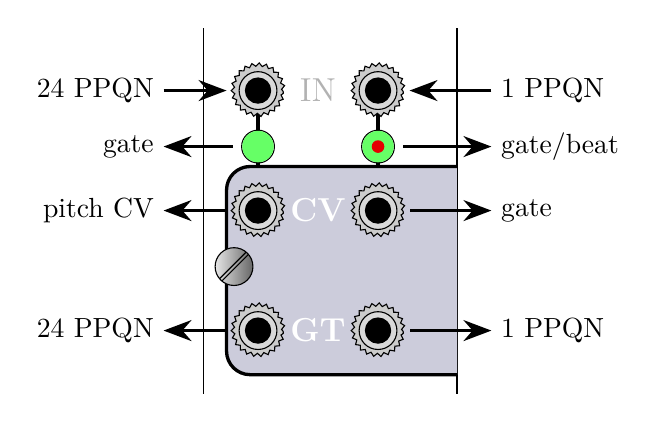
\begin{tikzpicture}[scale=0.8]
  {\setmainfont[Path={../../tsukurimashou/otf/},
BoldFont={TsukurimashouBokukkoExtraBoldPS}]{TsukurimashouBokukkoDemiboldPS}%
% start out defining coordinates
\coordinate (lbh) at (4.91mm,31.23mm) {};
\coordinate (j1) at (8.72mm,59.17mm) {};
\coordinate (j2) at (27.77mm,59.17mm) {};
\coordinate (j3) at (8.72mm,40.12mm) {};
\coordinate (j4) at (27.77mm,40.12mm) {};
\coordinate (j5) at (8.72mm,21.07mm) {};
\coordinate (j6) at (27.77mm,21.07mm) {};
\coordinate (d5) at (8.72mm,50.28mm) {};
\coordinate (d6) at (27.77mm,50.28mm) {};
%
\draw (0,11.07mm) -- (0,69.07mm);
\draw (40.30mm,11.07mm) -- (40.30mm,69.07mm);
%
\draw[very thick,black] (j1) -- (j3);
\draw[very thick,black] (j2) -- (j4);
\draw[very thick,black,fill=blue!30!black!20!white,rounded corners=3.0mm]
  (40.30mm,47.12mm) -- (3.72mm,47.12mm) --
  (3.72mm,14.07mm) -- (40.33mm,14.07mm);
\node[black!30!white] at ($(j1)!0.5!(j2)$) {\large IN};
\node[white] at ($(j3)!0.5!(j4)$) {\large\textbf{CV}};
\node[white] at ($(j5)!0.5!(j6)$) {\large\textbf{GT}};
%
% board-to-panel mounting holes, to clear M3 machine screw
\draw (lbh) circle[radius=1.60mm];
% six jacks with M6 threads, 6.3mm holes
\draw (j1) circle[radius=3.15mm];
\draw (j2) circle[radius=3.15mm];
\draw (j3) circle[radius=3.15mm];
\draw (j4) circle[radius=3.15mm];
\draw (j5) circle[radius=3.15mm];
\draw (j6) circle[radius=3.15mm];
% two LEDs, 5.20mm holes
\draw (d5) circle[radius=2.60mm];
\draw (d6) circle[radius=2.60mm];
%
% mock up screw heads, knobs
% machine screws with 6mm heads
\foreach \screwname in {lbh} {
  \path[draw=black,shading=ball,
    left color=black!10!white,right color=black!60!white]
    (\screwname) circle[radius=3mm];
  \draw ($(\screwname)+(50:3.0mm)$)--($(\screwname)+(220:3.0mm)$);
  \draw ($(\screwname)+(40:3.0mm)$)--($(\screwname)+(230:3.0mm)$);
}
% jacks with knurled nuts
\foreach \jackname in {j1,j2,j3,j4,j5,j6} {
  \path[draw=black,fill=black!20!white,
    decorate,decoration={snake,amplitude=0.6,segment length=2.5}]
    ($(\jackname)+(0,-0.15mm)$) circle[radius=4mm];
  \path[draw=black,fill=black!15!white] (\jackname) circle[radius=3mm];
  \path[draw=black,fill=black] (\jackname) circle[radius=2mm];
}
}

%
  \path[fill=green!60!white] (d5) circle[radius=2.50mm];
  \path[fill=green!60!white] (d6) circle[radius=2.50mm];
  \path[fill=red!90!black] (d6) circle[radius=1.0mm];
  \draw[very thick,-{Stealth[scale=1.2]}]
    ($(j1)+(-15mm,0)$) -- ($(j1)+(-5mm,0)$);
  \draw[very thick,-{Stealth[scale=1.2]}]
    ($(j2)+(18mm,0)$) -- ($(j2)+(5mm,0)$);
  \draw[very thick,{Stealth[scale=1.2]}-]
    ($(d5)+(-15mm,0)$) -- ($(d5)+(-4mm,0)$);
  \draw[very thick,{Stealth[scale=1.2]}-]
    ($(d6)+(18mm,0)$) -- ($(d6)+(4mm,0)$);
  \draw[very thick,{Stealth[scale=1.2]}-]
    ($(j3)+(-15mm,0)$) -- ($(j3)+(-5mm,0)$);
  \draw[very thick,{Stealth[scale=1.2]}-]
    ($(j4)+(18mm,0)$) -- ($(j4)+(5mm,0)$);
  \draw[very thick,{Stealth[scale=1.2]}-]
    ($(j5)+(-15mm,0)$) -- ($(j5)+(-5mm,0)$);
  \draw[very thick,{Stealth[scale=1.2]}-]
    ($(j6)+(18mm,0)$) -- ($(j6)+(5mm,0)$);
%
  \node[anchor=east] at ($(j1)+(-15mm,0)$) {24 PPQN};
  \node[anchor=west] at ($(j2)+(18mm,0)$) {1 PPQN};
  \node[anchor=east] at ($(d5)+(-15mm,0)$) {gate};
  \node[anchor=west] at ($(d6)+(18mm,0)$) {gate/beat};
  \node[anchor=east] at ($(j3)+(-15mm,0)$) {pitch CV};
  \node[anchor=west] at ($(j4)+(18mm,0)$) {gate};
  \node[anchor=east] at ($(j5)+(-15mm,0)$) {24 PPQN};
  \node[anchor=west] at ($(j6)+(18mm,0)$) {1 PPQN};
\end{tikzpicture}\par}

This channel implements monophonic note stealing, the same as Channel~1. 
Both LEDs glow green when a note is playing, but the right LED also flashes
red on the beat, overriding the green.

%%%%%%%%%%%%%%%%%%%%%%%%%%%%%%%%%%%%%%%%%%%%%%%%%%%%%%%%%%%%%%%%%%%%%%%%

\section{Channels 13--16:  reserved}

The last four channels are not currently implemented.  They are available
for use by future versions of the official firmware, or possibly by
user-defined firmware.

% $Id: qwerty.tex 9718 2021-12-19 19:26:46Z mskala $

%
% Typing (QWERTY) keyboard interface
% Copyright (C) 2022  Matthew Skala
%
% This program is free software: you can redistribute it and/or modify
% it under the terms of the GNU General Public License as published by
% the Free Software Foundation, version 3.
%
% This program is distributed in the hope that it will be useful,
% but WITHOUT ANY WARRANTY; without even the implied warranty of
% MERCHANTABILITY or FITNESS FOR A PARTICULAR PURPOSE.  See the
% GNU General Public License for more details.
%
% You should have received a copy of the GNU General Public License
% along with this program.  If not, see <http://www.gnu.org/licenses/>.
%
% Matthew Skala
% https://northcoastsynthesis.com/
% mskala@northcoastsynthesis.com
%

\newcommand{\myFlFl}{\raisebox{0.2ex}{\musDoubleFlat}}
\newcommand{\myFl}{\raisebox{0.2ex}{\musFlat}}
\newcommand{\mySh}{\raisebox{0.4ex}{\musSharp}}
\newcommand{\myShSh}{\raisebox{0.4ex}{\musDoubleSharp}}

\chapter{Typing keyboard interface}

The Gracious Host supports two kinds of USB keyboards:  musical keyboards
with a USB MIDI interface as described in the previous chapter, and the
other kind of keyboard that is commonly attached to a PC and used for
typing.  The driver for typing keyboards, described in this chapter, allows
them to be used for playing synthesizers -- with some limitations, but at a
much lower cost than most full-featured MIDI keyboards.

%%%%%%%%%%%%%%%%%%%%%%%%%%%%%%%%%%%%%%%%%%%%%%%%%%%%%%%%%%%%%%%%%%%%%%%%

\section{General comments on USB keyboards}

The typing keyboard driver supports what the USB standards call the ``boot
keyboard'' protocol.  In technical USB terms that means it will support a
USB device with an interface descriptor of class 3, subclass 1, protocol 1. 
This is the standard USB keyboard protocol used by the typing keyboards
people commonly plug into personal computers.  It is called ``boot
keyboard'' because the authors of the relevant standard apparently imagined
that the simple protocol would only be used by the BIOS configuration menus
of PCs, and most operating systems would instead use the ridiculously
complicated full-generality ``HID report protocol'' instead; but in fact,
most real-world implementations just use the boot keyboard protocol.

Wiring switches together to form a keyboard becomes more complicated if it
is desired to correctly detect when the user presses more than one key at
the same time.  In musical keyboards this issue is called ``polyphony'';
with typing keyboards, the same thing is called ``rollover.'' The USB boot
keyboard protocol is only capable of reporting to the host at most six
simultaneous keypresses (of regular typing keys; modifier keys like shift
are handled separately and do not count toward this limit) because it sends
six bytes of key information per report packet with each key consuming one
byte.  So a USB keyboard plugged into the Gracious Host can play \emph{at
most} six simultaneous MIDI notes in the ordinary way by pressing keys
at once.

However, reaching the limit requires keyboard hardware actually capable of
six-key rollover.  Some keyboards, especially fancier ones marketed as
``gaming'' keyboards, are able to do it; but cheaper generic USB keyboards
cannot really do full six-key rollover.  The average USB typing keyboard
that does not specifically advertise a rollover feature may give
incorrect results (not detecting some keys, or spuriously detecting
unpressed ``ghost'' keys) when multiple keys are pressed, usually depending
in a complicated way on the specific key combination involved.  The
Gracious Host only knows what the keyboard tells it, and cannot easily
compensate for such behaviour.

For the quantizer and arpeggiator features it's useful to play many notes at
once; so to get around both keyboard rollover limits and the user's limited
number of fingers, the Gracious Host typing-keyboard driver supports a
\emph{sustain} feature using the Caps Lock key to lock keys in a pressed
state without needing to hold them down.  See the section on that below.

USB typing keyboards have a limit on how fast they can be polled, and that
limits how responsive to keystrokes anything controlled by a USB typing
keyboard can be.  The limit depends on the specific keyboard model (the
keyboard decides how fast it will respond) but the default is usually
10ms intervals, for 100 polls per second.  There can also be a further delay
of a few milliseconds internal to the keyboard as the keyboard hardware
scans the array of switches.  Human beings are not capable of perceiving this
amount of so-called latency in keystroke response but many believe
they can, and users who hold that belief might prefer to use a USB MIDI
keyboard instead of a typing keyboard.  The USB MIDI protocol as implemented
by the Gracious Host allows for sub-millisecond polling.

The general layout of a USB typing keyboard is reasonably standardized, but
there are many small details that vary from one to another.  The biggest
distinction is between ``US-style'' keyboards, with a large L-shaped Enter
key, and ``ISO-style'' keyboards with a narrower vertical Enter key and a
few more small keys to accommodate the additional letters in non-English
languages.  The precise details of those keys, which letters are shown on
which keycaps, the locations of some punctuation marks like backslash, and
so on, vary a lot.  Keyboards do not report the details of their layout to a
USB host, so the host has to guess, maintain a database of specific keyboard
models, or be configured for it out-of-band.

The Gracious Host attempts to support all relevant keys that exist in most
popular keyboard layouts used around the world, with reasonable guesses as
to where they will be located; but be aware that it's possible your keyboard
will not actually have all the keys shown in the diagrams in this manual, or
that a few of them (especially around the edges of the main keyboard area)
will not be located exactly where they are shown.

The keys labelled ``GUI'' (and not implemented to do anything, in
the current firmware) are called that here because that's what they are
called in the relevant USB standard.  On most keyboards they are actually
labelled with the logo of an operating system vendor, like Microsoft or
Apple.

%%%%%%%%%%%%%%%%%%%%%%%%%%%%%%%%%%%%%%%%%%%%%%%%%%%%%%%%%%%%%%%%%%%%%%%%

\section{Piano-style keyboard layout}

Figure~\ref{fig:qwerty-layouts} shows two layouts.  The upper one is the
default layout active when a keyboard is first plugged into the Gracious
Host and the Num Lock LED is off.  Note names and MIDI note numbers
(assuming no octave shift) are as shown in the diagram.

\begin{sidewaysfigure*}
{\centering
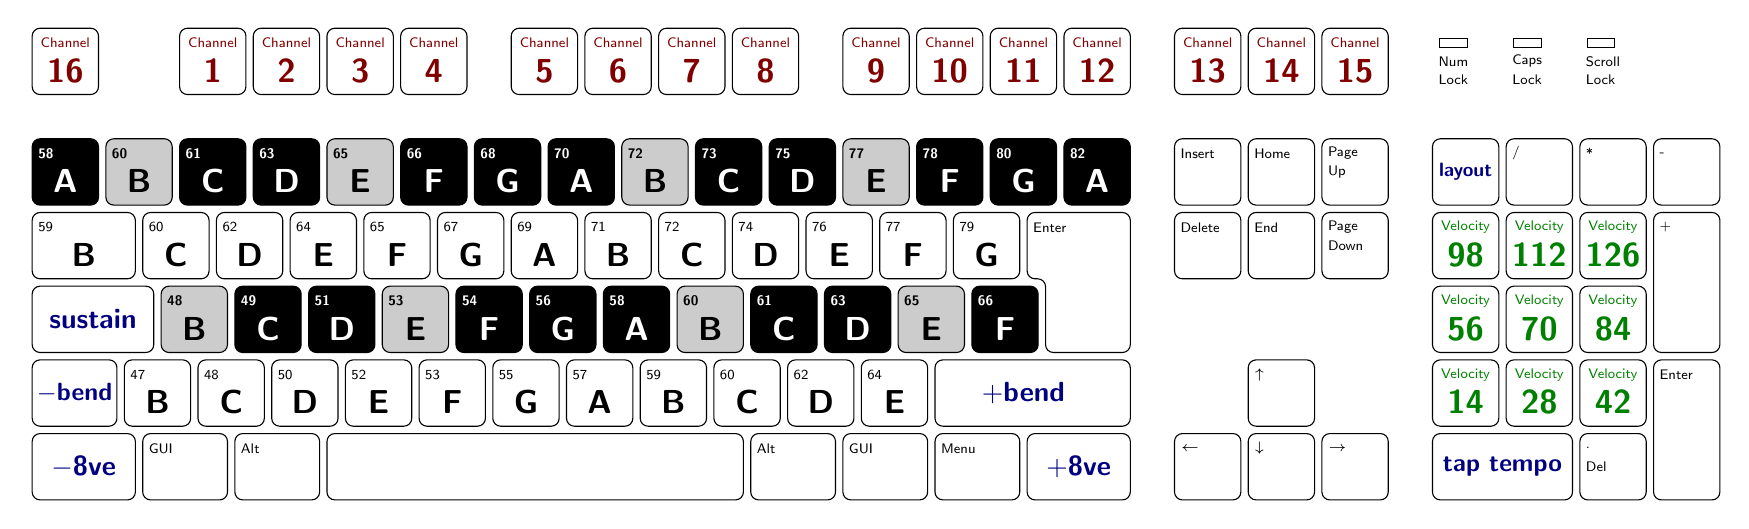
\begin{tikzpicture}[scale=0.234]
  % first row
  \foreach \xa/\xb/\tb in
    {0/4/16,
     8/12/1,12/16/2,16/20/3,20/24/4,
     26/30/5,30/34/6,34/38/7,38/42/8,
     44/48/9,48/52/10,52/56/11,56/60/12,
     62/66/13,66/70/14,70/74/15} {
    \draw[rounded corners={1mm}]
      ($(\xa,22)+(0.2,0.2)$) rectangle ($(\xb,26)+(-0.2,-0.2)$);
    \node[red!50!black] at ($(\xa,26)+(2,-1)$)
      {\tiny\textsf{Channel}};
    \node[red!50!black] at ($(\xa,22)+(2,1.5)$) {\large\bf\textsf{\tb}};
  }
  % LEDs
  \foreach \x/\t in {76/Num,80/Caps,84/Scroll} {
    \draw (\x+0.6,24.75) rectangle (\x+2.1,25.25);
    \node[anchor=west] at ($(\x,26)+(0,-2)$) {\tiny\textsf{\t}};
    \node[anchor=west] at ($(\x,26)+(0,-3)$) {\tiny\textsf{Lock}};
  }
  % second row, black note keys
  \foreach \xa/\xb/\ta/\tb in
    {0/4/58/{A\mySh},8/12/61/{C\mySh},12/16/63/{D\mySh},
     20/24/66/{F\mySh},24/28/68/{G\mySh},28/32/70/{A\mySh},
     36/40/73/{C\mySh},40/44/75/{D\mySh},48/52/78/{F\mySh},
     52/56/80/{G\mySh},56/60/82/{A\mySh}} {
    \draw[rounded corners={1mm},fill=black]
      ($(\xa,16)+(0.2,0.2)$) rectangle ($(\xb,20)+(-0.2,-0.2)$);
    \node[anchor=west,white] at ($(\xa,20)+(0,-1)$) {\tiny\bf\textsf{\ta}};
    \node[white] at ($(\xa,16)+(2,1.5)$) {\large\bf\textsf{\tb}};
  }
  % second row, skipped keys
  \foreach \xa/\xb/\ta/\tb in
    {4/8/60/{B\mySh},16/20/65/{E\mySh},32/36/72/{B\mySh},44/48/77/{E\mySh}} {
    \draw[rounded corners={1mm},fill=black!20!white]
      ($(\xa,16)+(0.2,0.2)$) rectangle ($(\xb,20)+(-0.2,-0.2)$);
    \node[anchor=west] at ($(\xa,20)+(0,-1)$) {\tiny\bf\textsf{\ta}};
    \node at ($(\xa,16)+(2,1.5)$) {\large\bf\textsf{\tb}};
  }
  % second row, non-note keys
  \foreach \xa/\xb/\ta/\tb in
    {62/66/Insert/{},66/70/Home/{},70/74/Page/Up,
     76/80/{}/{},80/84/{/}/{},84/88/*/{},88/92/-/{}} {
    \draw[rounded corners={1mm}]
      ($(\xa,16)+(0.2,0.2)$) rectangle ($(\xb,20)+(-0.2,-0.2)$);
    \node[anchor=west] at ($(\xa,20)+(0,-1)$) {\tiny\textsf{\ta}};
    \node[anchor=west] at ($(\xa,20)+(0,-2)$) {\tiny\textsf{\tb}};
  }
  % third row, white note keys
  \foreach \xa/\xb/\ta/\tb in
    {0/6/59/B,6/10/60/C,10/14/62/D,14/18/64/E,
     18/22/65/F,22/26/67/G,26/30/69/A,30/34/71/B,
     34/38/72/C,38/42/74/D,42/46/76/E,46/50/77/F,
     50/54/79/G} {
    \draw[rounded corners={1mm}]
      ($(\xa,12)+(0.2,0.2)$) rectangle ($(\xb,16)+(-0.2,-0.2)$);
    \node[anchor=west] at ($(\xa,16)+(0,-1)$) {\tiny\textsf{\ta}};
    \node at ($(\xa,12+1.5)!0.5!(\xb,12+1.5)$) {\large\bf\textsf{\tb}};
  }
  % third row, non-note keys
  \foreach \xa/\xb/\ta/\tb in
    {62/66/Delete/{},66/70/End/{},70/74/Page/Down} {
    \draw[rounded corners={1mm}]
      ($(\xa,12)+(0.2,0.2)$) rectangle ($(\xb,16)+(-0.2,-0.2)$);
    \node[anchor=west] at ($(\xa,16)+(0,-1)$) {\tiny\textsf{\ta}};
    \node[anchor=west] at ($(\xa,16)+(0,-2)$) {\tiny\textsf{\tb}};
  }
  % keys that span third and fourth rows
  \draw[rounded corners={1mm}]
    ($(55,8)+(0.2,0.2)$) -- ($(55,12)+(0.2,0.2)$) --
    ($(54,12)+(0.2,0.2)$) -- ($(54,16)+(0.2,-0.2)$) --
    ($(60,16)+(-0.2,-0.2)$) -- ($(60,8)+(-0.2,0.2)$) --cycle;
  \node[anchor=west] at ($(54,16)+(0,-1)$) {\tiny\textsf{Enter}};
  \draw[rounded corners={1mm}]
    ($(88,8)+(0.2,0.2)$) rectangle ($(92,16)+(-0.2,-0.2)$);
  \node[anchor=west] at ($(88,16)+(0,-1)$) {\tiny\textsf{+}};
  % fourth row, black note keys
  \foreach \xa/\xb/\ta/\tb in
    {11/15/49/{C\mySh},15/19/51/{D\mySh},
     23/27/54/{F\mySh},27/31/56/{G\mySh},31/35/58/{A\mySh},
     39/43/61/{C\mySh},43/47/63/{D\mySh},
     51/55/66/{F\mySh}} {
    \draw[rounded corners={1mm}, fill=black]
      ($(\xa,8)+(0.2,0.2)$) rectangle ($(\xb,12)+(-0.2,-0.2)$);
    \node[anchor=west,white] at ($(\xa,12)+(0,-1)$) {\tiny\bf\textsf{\ta}};
    \node[white] at ($(\xa,8)+(2,1.5)$) {\large\bf\textsf{\tb}};
  }
  % fourth row, skipped keys
  \foreach \xa/\xb/\ta/\tb in
    {7/11/48/{B\mySh},
     19/23/53/{E\mySh},
     35/39/60/{B\mySh},47/51/65/{E\mySh}} {
    \draw[rounded corners={1mm},fill=black!20!white]
      ($(\xa,8)+(0.2,0.2)$) rectangle ($(\xb,12)+(-0.2,-0.2)$);
    \node[anchor=west] at ($(\xa,12)+(0,-1)$) {\tiny\bf\textsf{\ta}};
    \node at ($(\xa,8)+(2,1.5)$) {\large\bf\textsf{\tb}};
  }
  % fourth row, non-note keys
  \foreach \xa/\xb/\ta/\tb in
    {0/7/{}/{}} {
    \draw[rounded corners={1mm}]
      ($(\xa,8)+(0.2,0.2)$) rectangle ($(\xb,12)+(-0.2,-0.2)$);
    \node[anchor=west] at ($(\xa,12)+(0,-1)$) {\tiny\textsf{\ta}};
    \node[anchor=west] at ($(\xa,12)+(0,-2)$) {\tiny\textsf{\tb}};
  }
  % fifth row, white note keys
  \foreach \xa/\xb/\ta/\tb in
    {5/9/47/B,9/13/48/C,13/17/50/D,17/21/52/E,
     21/25/53/F,25/29/55/G,29/33/57/A,33/37/59/B,
     37/41/60/C,41/45/62/D,45/49/64/E} {
    \draw[rounded corners={1mm}]
      ($(\xa,4)+(0.2,0.2)$) rectangle ($(\xb,8)+(-0.2,-0.2)$);
    \node[anchor=west] at ($(\xa,8)+(0,-1)$) {\tiny\textsf{\ta}};
    \node at ($(\xa,4+1.5)!0.5!(\xb,4+1.5)$) {\large\bf\textsf{\tb}};
  }
  % fifth row, non-note keys
  \foreach \xa/\xb/\ta/\tb in
    {0/5/{}/{},49/60/{}/{},
     66/70/{$\uparrow$}/{}} {
    \draw[rounded corners={1mm}]
      ($(\xa,4)+(0.2,0.2)$) rectangle ($(\xb,8)+(-0.2,-0.2)$);
    \node[anchor=west] at ($(\xa,8)+(0,-1)$) {\tiny\textsf{\ta}};
    \node[anchor=west] at ($(\xa,8)+(0,-2)$) {\tiny\textsf{\tb}};
  }
  % keys that span fifth and sixth rows
  \draw[rounded corners={1mm}]
    ($(88,0)+(0.2,0.2)$) rectangle ($(92,8)+(-0.2,-0.2)$);
  \node[anchor=west] at ($(88,8)+(0,-1)$) {\tiny\textsf{Enter}};
  % sixth row
  \foreach \xa/\xb/\ta/\tb in
    {0/6/{}/{},6/11/GUI/{},11/16/Alt/{},16/39/{}/{},
     39/44/Alt/{},44/49/GUI/{},49/54/Menu/{},54/60/{}/{},
     62/66/{$\leftarrow$}/{},66/70/{$\downarrow$}/{},70/74/{$\rightarrow$}/{},
     76/84/{}/{},84/88/./Del} {
    \draw[rounded corners={1mm}]
      ($(\xa,0)+(0.2,0.2)$) rectangle ($(\xb,4)+(-0.2,-0.2)$);
    \node[anchor=west] at ($(\xa,4)+(0,-1)$) {\tiny\textsf{\ta}};
    \node[anchor=west] at ($(\xa,4)+(0,-2)$) {\tiny\textsf{\tb}};
  }
  % keypad numerals
  \foreach \x/\y/\t in {76/4/14,80/4/28,84/4/42,76/8/56,80/8/70,
    84/8/84,76/12/98,80/12/112,84/12/126} {
    \draw[rounded corners={1mm}]
      ($(\x,\y)+(0.2,0.2)$) rectangle ($(\x+4,\y+4)+(-0.2,-0.2)$);
    \node[green!50!black] at ($(\x,\y)+(2,3)$)
      {\tiny\textsf{Velocity}};
    \node[green!50!black] at ($(\x,\y)+(2,1.5)$) {\large\bf\textsf{\t}};
  }
  % additional key labels
  \node[blue!50!black] at (3.5,10) {\bf\textsf{sustain}};
  \node[blue!50!black] at (2.5,6) {\small\bf\textsf{$-$bend}};
  \node[blue!50!black] at (3,2) {\bf\textsf{$-$8ve}};
  \node[blue!50!black] at (54,6) {\bf\textsf{$+$bend}};
  \node[blue!50!black] at (57,2) {\bf\textsf{$+$8ve}};
  \node[blue!50!black] at (78,18) {\scriptsize\bf\textsf{layout}};
  \node[blue!50!black] at (80,2) {\small\bf\textsf{tap tempo}};
\end{tikzpicture}\par
\vspace*{60pt}
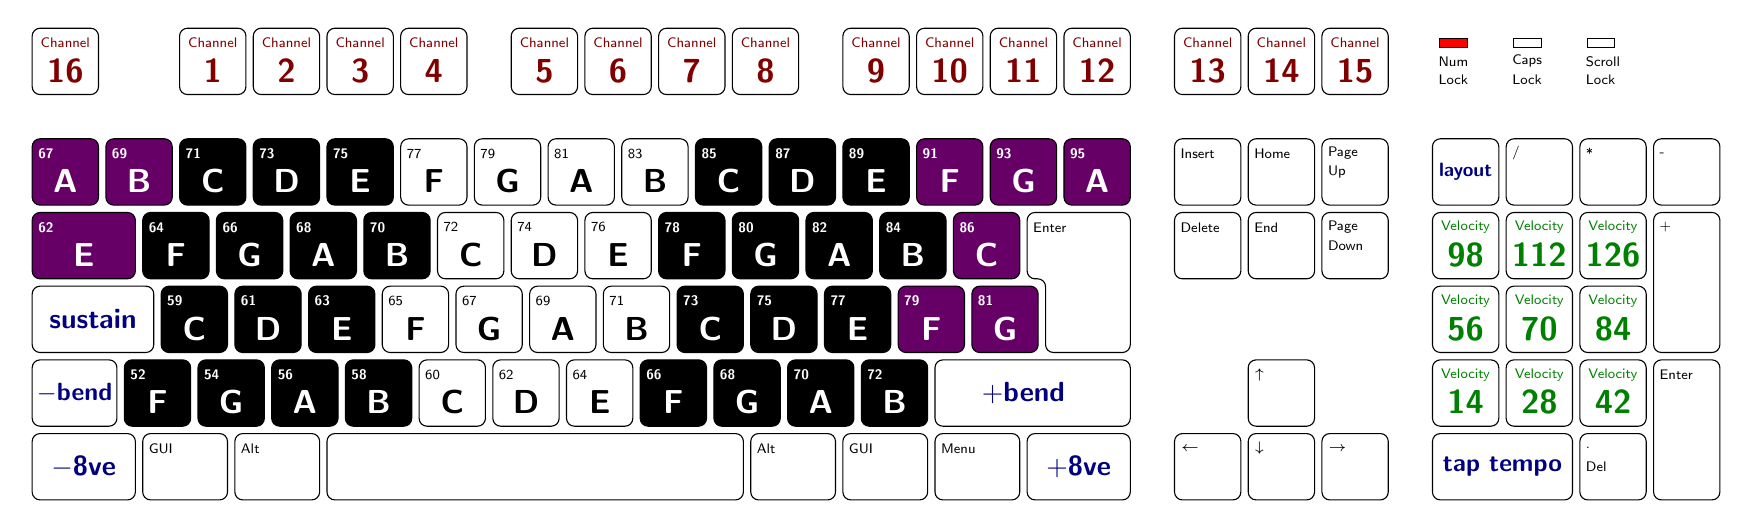
\begin{tikzpicture}[scale=0.234]
  % first row
  \foreach \xa/\xb/\tb in
    {0/4/16,
     8/12/1,12/16/2,16/20/3,20/24/4,
     26/30/5,30/34/6,34/38/7,38/42/8,
     44/48/9,48/52/10,52/56/11,56/60/12,
     62/66/13,66/70/14,70/74/15} {
    \draw[rounded corners={1mm}]
      ($(\xa,22)+(0.2,0.2)$) rectangle ($(\xb,26)+(-0.2,-0.2)$);
    \node[red!50!black] at ($(\xa,26)+(2,-1)$)
      {\tiny\textsf{Channel}};
    \node[red!50!black] at ($(\xa,22)+(2,1.5)$) {\large\bf\textsf{\tb}};
  }
  % LEDs
  \foreach \x/\t in {80/Caps,84/Scroll} {
    \draw (\x+0.6,24.75) rectangle (\x+2.1,25.25);
    \node[anchor=west] at ($(\x,26)+(0,-2)$) {\tiny\textsf{\t}};
    \node[anchor=west] at ($(\x,26)+(0,-3)$) {\tiny\textsf{Lock}};
  }
  \draw[fill=red] (76+0.6,24.75) rectangle (76+2.1,25.25);
  \node[anchor=west] at ($(76,26)+(0,-2)$) {\tiny\textsf{Num}};
  \node[anchor=west] at ($(76,26)+(0,-3)$) {\tiny\textsf{Lock}};
  % second row, purple note keys
  \foreach \xa/\xb/\ta/\tb in
    {0/4/67/{A\myFlFl},4/8/69/{B\myFlFl},48/52/91/{F\myShSh},
     52/56/93/{G\myShSh},56/60/95/{A\myShSh}} {
    \draw[rounded corners={1mm},fill=red!50!blue!80!black]
      ($(\xa,16)+(0.2,0.2)$) rectangle ($(\xb,20)+(-0.2,-0.2)$);
    \node[anchor=west,white] at ($(\xa,20)+(0,-1)$) {\tiny\bf\textsf{\ta}};
    \node[white] at ($(\xa,16)+(2,1.5)$) {\large\bf\textsf{\tb}};
  }
  % second row, black note keys
  \foreach \xa/\xb/\ta/\tb in
    {8/12/71/{C\myFl},12/16/73/{D\myFl},16/20/75/{E\myFl},
     36/40/85/{C\mySh},40/44/87/{D\mySh},44/48/89/{E\mySh}} {
    \draw[rounded corners={1mm},fill=black]
      ($(\xa,16)+(0.2,0.2)$) rectangle ($(\xb,20)+(-0.2,-0.2)$);
    \node[anchor=west,white] at ($(\xa,20)+(0,-1)$) {\tiny\bf\textsf{\ta}};
    \node[white] at ($(\xa,16)+(2,1.5)$) {\large\bf\textsf{\tb}};
  }
  % second row, white note keys
  \foreach \xa/\xb/\ta/\tb in
    {20/24/77/F,24/28/79/G,28/32/81/A,32/36/83/B} {
    \draw[rounded corners={1mm}]
      ($(\xa,16)+(0.2,0.2)$) rectangle ($(\xb,20)+(-0.2,-0.2)$);
    \node[anchor=west] at ($(\xa,20)+(0,-1)$) {\tiny\textsf{\ta}};
    \node at ($(\xa,16)+(2,1.5)$) {\large\bf\textsf{\tb}};
  }
  % second row, non-note keys
  \foreach \xa/\xb/\ta/\tb in
    {62/66/Insert/{},66/70/Home/{},70/74/Page/Up,
     76/80/{}/{},80/84/{/}/{},84/88/*/{},88/92/-/{}} {
    \draw[rounded corners={1mm}]
      ($(\xa,16)+(0.2,0.2)$) rectangle ($(\xb,20)+(-0.2,-0.2)$);
    \node[anchor=west] at ($(\xa,20)+(0,-1)$) {\tiny\textsf{\ta}};
    \node[anchor=west] at ($(\xa,20)+(0,-2)$) {\tiny\textsf{\tb}};
  }
  % third row, purple note keys
  \foreach \xa/\xb/\ta/\tb in
    {0/6/62/{E\myFlFl},50/54/86/{C\myShSh}} {
    \draw[rounded corners={1mm},fill=red!50!blue!80!black]
      ($(\xa,12)+(0.2,0.2)$) rectangle ($(\xb,16)+(-0.2,-0.2)$);
    \node[anchor=west,white] at ($(\xa,16)+(0,-1)$) {\tiny\bf\textsf{\ta}};
    \node[white] at ($(\xa,12+1.5)!0.5!(\xb,12+1.5)$) {\large\bf\textsf{\tb}};
  }
  % third row, black note keys
  \foreach \xa/\xb/\ta/\tb in
    {6/10/64/{F\myFl},10/14/66/{G\myFl},14/18/68/{A\myFl},18/22/70/{B\myFl},
     34/38/78/{F\mySh},38/42/80/{G\mySh},42/46/82/{A\mySh},46/50/84/{B\mySh}} {
    \draw[rounded corners={1mm},fill=black]
      ($(\xa,12)+(0.2,0.2)$) rectangle ($(\xb,16)+(-0.2,-0.2)$);
    \node[anchor=west,white] at ($(\xa,16)+(0,-1)$) {\tiny\bf\textsf{\ta}};
    \node[white] at ($(\xa,12+1.5)!0.5!(\xb,12+1.5)$) {\large\bf\textsf{\tb}};
  }
  % third row, white note keys
  \foreach \xa/\xb/\ta/\tb in
    {22/26/72/C,26/30/74/D,30/34/76/E} {
    \draw[rounded corners={1mm}]
      ($(\xa,12)+(0.2,0.2)$) rectangle ($(\xb,16)+(-0.2,-0.2)$);
    \node[anchor=west] at ($(\xa,16)+(0,-1)$) {\tiny\textsf{\ta}};
    \node at ($(\xa,12+1.5)!0.5!(\xb,12+1.5)$) {\large\bf\textsf{\tb}};
  }
  % third row, non-note keys
  \foreach \xa/\xb/\ta/\tb in
    {62/66/Delete/{},66/70/End/{},70/74/Page/Down} {
    \draw[rounded corners={1mm}]
      ($(\xa,12)+(0.2,0.2)$) rectangle ($(\xb,16)+(-0.2,-0.2)$);
    \node[anchor=west] at ($(\xa,16)+(0,-1)$) {\tiny\textsf{\ta}};
    \node[anchor=west] at ($(\xa,16)+(0,-2)$) {\tiny\textsf{\tb}};
  }
  % keys that span third and fourth rows
  \draw[rounded corners={1mm}]
    ($(55,8)+(0.2,0.2)$) -- ($(55,12)+(0.2,0.2)$) --
    ($(54,12)+(0.2,0.2)$) -- ($(54,16)+(0.2,-0.2)$) --
    ($(60,16)+(-0.2,-0.2)$) -- ($(60,8)+(-0.2,0.2)$) --cycle;
  \node[anchor=west] at ($(54,16)+(0,-1)$) {\tiny\textsf{Enter}};
  \draw[rounded corners={1mm}]
    ($(88,8)+(0.2,0.2)$) rectangle ($(92,16)+(-0.2,-0.2)$);
  \node[anchor=west] at ($(88,16)+(0,-1)$) {\tiny\textsf{+}};
  % fourth row, purple note keys
  \foreach \xa/\xb/\ta/\tb in
    {47/51/79/{F\myShSh},51/55/81/{G\myShSh}} {
    \draw[rounded corners={1mm},fill=red!50!blue!80!black]
      ($(\xa,8)+(0.2,0.2)$) rectangle ($(\xb,12)+(-0.2,-0.2)$);
    \node[anchor=west,white] at ($(\xa,12)+(0,-1)$) {\tiny\bf\textsf{\ta}};
    \node[white] at ($(\xa,8+1.5)!0.5!(\xb,8+1.5)$) {\large\bf\textsf{\tb}};
  }
  % fourth row, black note keys
  \foreach \xa/\xb/\ta/\tb in
    {7/11/59/{C\myFl},11/15/61/{D\myFl},15/19/63/{E\myFl},
     35/39/73/{C\mySh},39/43/75/{D\mySh},43/47/77/{E\mySh}} {
    \draw[rounded corners={1mm},fill=black]
      ($(\xa,8)+(0.2,0.2)$) rectangle ($(\xb,12)+(-0.2,-0.2)$);
    \node[anchor=west,white] at ($(\xa,12)+(0,-1)$) {\tiny\bf\textsf{\ta}};
    \node[white] at ($(\xa,8+1.5)!0.5!(\xb,8+1.5)$) {\large\bf\textsf{\tb}};
  }
  % fourth row, white note keys
  \foreach \xa/\xb/\ta/\tb in
    {0/7/{}/{},19/23/65/F,23/27/67/G,27/31/69/A,31/35/71/B} {
    \draw[rounded corners={1mm}]
      ($(\xa,8)+(0.2,0.2)$) rectangle ($(\xb,12)+(-0.2,-0.2)$);
    \node[anchor=west] at ($(\xa,12)+(0,-1)$) {\tiny\textsf{\ta}};
    \node at ($(\xa,8+1.5)!0.5!(\xb,8+1.5)$) {\large\bf\textsf{\tb}};
  }
  % fifth row, black note keys
  \foreach \xa/\xb/\ta/\tb in
    {5/9/52/{F\myFl},9/13/54/{G\myFl},13/17/56/{A\myFl},17/21/58/{B\myFl},
     33/37/66/{F\mySh},37/41/68/{G\mySh},41/45/70/{A\mySh},45/49/72/{B\mySh}} {
    \draw[rounded corners={1mm},fill=black]
      ($(\xa,4)+(0.2,0.2)$) rectangle ($(\xb,8)+(-0.2,-0.2)$);
    \node[anchor=west,white] at ($(\xa,8)+(0,-1)$) {\tiny\bf\textsf{\ta}};
    \node[white] at ($(\xa,4+1.5)!0.5!(\xb,4+1.5)$) {\large\bf\textsf{\tb}};
  }
  % fifth row, white note keys
  \foreach \xa/\xb/\ta/\tb in
    {21/25/60/C,25/29/62/D,29/33/64/E} {
    \draw[rounded corners={1mm}]
      ($(\xa,4)+(0.2,0.2)$) rectangle ($(\xb,8)+(-0.2,-0.2)$);
    \node[anchor=west] at ($(\xa,8)+(0,-1)$) {\tiny\textsf{\ta}};
    \node at ($(\xa,4+1.5)!0.5!(\xb,4+1.5)$) {\large\bf\textsf{\tb}};
  }
  % fifth row, non-note keys
  \foreach \xa/\xb/\ta/\tb in
    {0/5/{}/{},49/60/{}/{},
     66/70/{$\uparrow$}/{}} {
    \draw[rounded corners={1mm}]
      ($(\xa,4)+(0.2,0.2)$) rectangle ($(\xb,8)+(-0.2,-0.2)$);
    \node[anchor=west] at ($(\xa,8)+(0,-1)$) {\tiny\textsf{\ta}};
    \node[anchor=west] at ($(\xa,8)+(0,-2)$) {\tiny\textsf{\tb}};
  }
  % keys that span fifth and sixth rows
  \draw[rounded corners={1mm}]
    ($(88,0)+(0.2,0.2)$) rectangle ($(92,8)+(-0.2,-0.2)$);
  \node[anchor=west] at ($(88,8)+(0,-1)$) {\tiny\textsf{Enter}};
  % sixth row
  \foreach \xa/\xb/\ta/\tb in
    {0/6/{}/{},6/11/GUI/{},11/16/Alt/{},16/39/{}/{},
     39/44/Alt/{},44/49/GUI/{},49/54/Menu/{},54/60/{}/{},
     62/66/{$\leftarrow$}/{},66/70/{$\downarrow$}/{},70/74/{$\rightarrow$}/{},
     76/84/{}/{},84/88/./Del} {
    \draw[rounded corners={1mm}]
      ($(\xa,0)+(0.2,0.2)$) rectangle ($(\xb,4)+(-0.2,-0.2)$);
    \node[anchor=west] at ($(\xa,4)+(0,-1)$) {\tiny\textsf{\ta}};
    \node[anchor=west] at ($(\xa,4)+(0,-2)$) {\tiny\textsf{\tb}};
  }
  % keypad numerals
  \foreach \x/\y/\t in {76/4/14,80/4/28,84/4/42,76/8/56,80/8/70,
    84/8/84,76/12/98,80/12/112,84/12/126} {
    \draw[rounded corners={1mm}]
      ($(\x,\y)+(0.2,0.2)$) rectangle ($(\x+4,\y+4)+(-0.2,-0.2)$);
    \node[green!50!black] at ($(\x,\y)+(2,3)$)
      {\tiny\textsf{Velocity}};
    \node[green!50!black] at ($(\x,\y)+(2,1.5)$) {\large\bf\textsf{\t}};
  }
  % additional key labels
  \node[blue!50!black] at (3.5,10) {\bf\textsf{sustain}};
  \node[blue!50!black] at (2.5,6) {\small\bf\textsf{$-$bend}};
  \node[blue!50!black] at (3,2) {\bf\textsf{$-$8ve}};
  \node[blue!50!black] at (54,6) {\bf\textsf{$+$bend}};
  \node[blue!50!black] at (57,2) {\bf\textsf{$+$8ve}};
  \node[blue!50!black] at (78,18) {\scriptsize\bf\textsf{layout}};
  \node[blue!50!black] at (80,2) {\small\bf\textsf{tap tempo}};
\end{tikzpicture}\par
\vspace*{24pt}}
\caption{Keyboard layouts.}\label{fig:qwerty-layouts}
\end{sidewaysfigure*}

This layout is meant to imitate a piano's keyboard layout, with a little
over 2$\tfrac{1}{2}$ octaves of coverage.  Keys that fall into gaps of the
piano layout (shown in grey) are assigned to B$\musSharp$ and E$\musSharp$
(enharmonic to C and F) to make a consistent pattern.  The upper left of the
main letter area (Q on a QWERTY layout) is Middle~C, and the F key in a
QWERTY layout, which often has a tactile guide bump on it, is effectively an
F (shown as E$\musSharp$, but the same MIDI number).

%%%%%%%%%%%%%%%%%%%%%%%%%%%%%%%%%%%%%%%%%%%%%%%%%%%%%%%%%%%%%%%%%%%%%%%%

\section{Wicki-Hayden isomorphic layout}

Press Num Lock to switch layouts.  With the Num Lock LED glowing, the
Gracious Host implements a Wicki-Hayden isomorphic keyboard layout, as shown
in the lower half of Figure~\ref{fig:qwerty-layouts}.  This layout is named
after Kaspar Wicki and Brian Hayden, who independently invented and patented
it in 1896 and 1986 respectively.  It is similar to the layout commonly used
for concertina keyboards.

The Wicki-Hayden layout treats the keys as an hexagonal grid. 
Horizontally adjacent keys are a major second (two semitones) apart, pitch
going up from left to right across the keyboard.  From any note the
diagonally adjacent notes to the right represent the fifth of the note, in
the higher or lower octave according to whether they are diagonally up
and right or down and right.  Similarly, the diagonal notes to the left are
the fourth of the current note.  And going directly up or down two rows
corresponds to going up or down by a whole octave.

{\center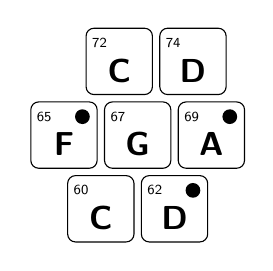
\begin{tikzpicture}[scale=0.234]
  \foreach \xa/\xb/\ta/\tb in
    {22/26/72/C,26/30/74/D} {
    \draw[rounded corners={1mm}]
      ($(\xa,12)+(0.2,0.2)$) rectangle ($(\xb,16)+(-0.2,-0.2)$);
    \node[anchor=west] at ($(\xa,16)+(0,-1)$) {\tiny\textsf{\ta}};
    \node at ($(\xa,12+1.5)!0.5!(\xb,12+1.5)$) {\large\bf\textsf{\tb}};
  }
  \foreach \xa/\xb/\ta/\tb in
    {19/23/65/F,23/27/67/G,27/31/69/A} {
    \draw[rounded corners={1mm}]
      ($(\xa,8)+(0.2,0.2)$) rectangle ($(\xb,12)+(-0.2,-0.2)$);
    \node[anchor=west] at ($(\xa,12)+(0,-1)$) {\tiny\textsf{\ta}};
    \node at ($(\xa,8+1.5)!0.5!(\xb,8+1.5)$) {\large\bf\textsf{\tb}};
  }
  \foreach \xa/\xb/\ta/\tb in
    {21/25/60/C,25/29/62/D} {
    \draw[rounded corners={1mm}]
      ($(\xa,4)+(0.2,0.2)$) rectangle ($(\xb,8)+(-0.2,-0.2)$);
    \node[anchor=west] at ($(\xa,8)+(0,-1)$) {\tiny\textsf{\ta}};
    \node at ($(\xa,4+1.5)!0.5!(\xb,4+1.5)$) {\large\bf\textsf{\tb}};
  }
  \fill (22,11) circle[radius=0.4];
  \fill (30,11) circle[radius=0.4];
  \fill (28,7) circle[radius=0.4];
\end{tikzpicture}\par}

The defining feature of an \emph{isomorphic}\footnote{This word means ``same
shape.''} music keyboard is that the harmonic relationships are the same
everywhere on the keyboard.  If you memorize the shape for a given chord
such as D~minor, shown by the dots above, you can play any chord of the same
quality, such as C~minor, by shifting the same shape somewhere else on the
keyboard.  These chords would have to be learned separately on a piano,
where D~minor is played entirely on white keys and C~minor involves a black
key.  Melodies can be transposed on an isomorphic keyboard just by moving to
a different physical location without changing the fingering.

With no octave shift, the Gracious Host's Wicki-Hayden layout puts the F
and G above Middle~C on the F and G keys of a standard QWERTY layout.

%%%%%%%%%%%%%%%%%%%%%%%%%%%%%%%%%%%%%%%%%%%%%%%%%%%%%%%%%%%%%%%%%%%%%%%%

\section{Sustain}

The Caps Lock key activates the \emph{sustain} feature.  Modes like
quantizer and arpeggiator benefit from being able to play many MIDI notes at
once; but both because people usually have at most ten fingers, and because
USB typing keyboards are limited in how many simultaneous keypresses they
can handle, actually pressing many note keys at once may be a problem.  The
basic sustain function is that when Caps Lock is pressed, the associated LED
goes on, and then all note keys pressed at that time or while Caps Lock
remains pressed, are locked.  These notes remain in effect even if the note
keys are released.  When Caps Lock is pressed a second time and the LED goes
off, all the locked notes are considered released at once.

The usual performace practice would be to either hold a chord and tap
Caps Lock to lock it; or to press and hold Caps Lock, and while holding it
build up the chord one or a few notes at a time before releasing Caps Lock.

In more detail:  Notes become locked if they are playing at the moment the
Caps Lock key is first pressed to activate sustain.  They also become locked
if they are newly pressed \emph{during} that first press of Caps Lock, so
the sequence ``press Caps Lock and hold; press note key; release Caps Lock''
results in the note being locked, regardless of exactly when the note key is
released.  Once locked, notes remain locked, and no additional Note On
events will be sent, until the second Caps Lock keypress, which will turn
off the LED and send Note Off events all at once for all the locked notes
except those that may actually be pressed at the moment of the second Caps
Lock keypress (which instead will be released when the note keys are
actually released).  After the first time Caps Lock has been released, with
the LED on and some notes held, other notes can be played normally. 
Re-playing a note already held will have no additional effect -- no second
Note On will be sent -- except that a note whose key is actually pressed
when releasing sustain will not get a Note Off at the release of sustain,
but only when its key is also released.

The sustain feature remembers the current channel when it is activated.  If
you change the channel while sustain is active, notes played in the new
channel are completely separate.  New Note On messages may be sent in the
new channel, and the eventual Note Offs when sustain is released will be
sent in the original channel.  Also, sustain is associated with \emph{note
numbers}, not with \emph{physical keyboard keys}.  By changing the octave
shift or the piano/isomorphic layout selection at different points in the
use of the sustain feature, it is quite possible for the same note key to
end up causing more than one note to be locked.

%%%%%%%%%%%%%%%%%%%%%%%%%%%%%%%%%%%%%%%%%%%%%%%%%%%%%%%%%%%%%%%%%%%%%%%%

\section{Octave shift}

The two Ctrl keys on the USB keyboard control octave shift.  Press the left
Ctrl key (just press like a normal key; it is not necessary to hold it down,
or press other keys along with it) to shift down one octave.  The typing
keys that send MIDI notes will send notes one octave lower than their
default values.  Press the right Ctrl to shift one octave up.  The Scroll
Lock LED will glow (as well as possibly blinking with the beat, see ``tap
tempo'' below) whenever an octave shift in either direction is active.

Pressing the shift keys again, shifts further.  Shifting up to five octaves
down or four octaves up is allowed, those limits being chosen to allow
covering the range of MIDI notes 1 to 127 in either keyboard layout, even on
a US-style keyboard with relatively few keys.  However, in practice it will
seldom be useful to play notes outside the range 24\ldots 96, which
corresponds to the range of the control voltage output DACs.

%%%%%%%%%%%%%%%%%%%%%%%%%%%%%%%%%%%%%%%%%%%%%%%%%%%%%%%%%%%%%%%%%%%%%%%%

\section{Pitch bend}

The right and left Shift keys send MIDI pitch bend messages.  The pitch will
bend up or down while you hold either Shift key (cancelling out, if both) up
to its default limit of two semitones, then will return once the Shift key
is released.  The speed of bend and return is fixed in the firmware; to
achieve finer control of pitch bend you need a proper MIDI controller
with this feature.

%%%%%%%%%%%%%%%%%%%%%%%%%%%%%%%%%%%%%%%%%%%%%%%%%%%%%%%%%%%%%%%%%%%%%%%%

\section{Channel selection}

Each function key (F1, F2, and so on) corresponds to the MIDI channel with
the same number.  Press one of these keys to set the channel on which the
typing keyboard will send subsequent MIDI events.  See the previous chapter
of this manual for descriptions of the different channels.  You can, for
instance, press F2 to switch to duophonic mode, or F10 to send drum
triggers.  Channel~1 is the default when the typing keyboard is first
connected, before any function key has been pressed.

The remaining keys in the function-key row select the remaining channels:
Print Screen, Scroll Lock, and Pause/Break (at the right of the row)
correspond to Channels~13, 14, and~15 as if they were F13, F14, and F15; and
Esc (usually at the left of the row, though it appears elsewhere on some
keyboards) to Channel~16 as if it were F16.  However, in the current
firmware as of this writing, channels beyond~12 do not actually do
anything.

Note that the MIDI subsystem determines its mode from \emph{the channel of
the most recent Note On message}.  Just pressing a function key to change
channels will not change the MIDI subsystem's mode; you must press a note
key to send a Note On before the MIDI subsystem will change modes.  The
concept here is that the module implements a MIDI to CV interface.  When you
plug in a typing keyboard, the typing keyboard is just a funny-looking MIDI
master keyboard plugged into the interface.  The function keys are
configuration commands to the keyboard regarding what channel it should send
MIDI messages on in the future; they are not MIDI messages in themselves. 
The MIDI subsystem, to the extent possible, responds to MIDI messages from a
typing keyboard just the same way it would respond to MIDI messages from a
music keyboard.

%%%%%%%%%%%%%%%%%%%%%%%%%%%%%%%%%%%%%%%%%%%%%%%%%%%%%%%%%%%%%%%%%%%%%%%%

\section{Velocity}

The keypad numerals 1 through 9 set the velocity for MIDI Note On events. 
Press any of these to choose the velocity for any subsequent notes.  The
values are as shown in the keyboard layout diagram, equal to the keycap
numeral value times 14, to provide equally spaced values throughout the MIDI
range.  Velocity is only relevant to Channel~1 (where it will be a control
voltage appearing on the right analog output) with the default firmware, but
some customized or future firmware might use velocity in other channels in
some way.

%%%%%%%%%%%%%%%%%%%%%%%%%%%%%%%%%%%%%%%%%%%%%%%%%%%%%%%%%%%%%%%%%%%%%%%%

\section{Tap tempo}

The keypad Insert (0) key functions as \emph{tap tempo}.  This allows the
performer to establish a clock for the arpeggiator and sync modes without
needing to patch in a clock control voltage signal.  In some channel modes
the resulting clock appears as a control voltage output and can be used to
control other modules.  Although there are some differences in the internal
implementation, the tap tempo feature basically serves the same purpose as
MIDI Timing Clock messages (24 of those per tap).

Press the tap tempo key at least twice, on the desired beat, to start the
tempo clock.  The Scroll Lock LED will blink on the beat (overlaid on its
solid glow, if octave shift is active).  If you enter three or more taps, in
a reasonably consistent straight rhythm, the tempo will be determined by an
exponential moving average of the most recent timings; that allows for a
more precise fit than would be possible by using only the two most recent,
given the limited precision of USB keyboard timing.  A tap that is not close
to the established timing, or that seems to have skipped at least one beat,
will be treated as the start of a new tap tempo sequence, stopping the old
clock.

%%%%%%%%%%%%%%%%%%%%%%%%%%%%%%%%%%%%%%%%%%%%%%%%%%%%%%%%%%%%%%%%%%%%%%%%

\section{Maintenance codes}

It is possible to activate special features, mostly intended for firmware
testing, by entering a four-digit decimal number through the typing
keyboard driver.  The only maintenance code that most module owners will
find really useful is 5833, to run the calibration procedure.  But for
completeness, here is a list of all the codes supported by production
firmware.

\begin{description}
\item[5833] Run the calibration procedure.
\item[1240] Simulate USB hub insertion (blinks ``H'' in Morse code).
\item[3627] Simulate insertion of an unsupported USB device (blinks ``D'' in
Morse code).
\item[4935] Perform the ``success'' display (normally done as the result of a
completed calibration).
\item[6697] Perform the ``failure'' display (normally the result of an aborted
calibration).
\item[8189] Throw a driver exception (flashes lights and waits for USB
disconnect).
\item[8605] Simulate a power-on reset.
\end{description}

Special firmware assembled with test routines included will also accept a
few other codes to run the test routines, but those will have no effect on
standard production firmware.  See the \emph{Gracious Host Programmer's
Manual} for details on compiling test firmware, and how to
create your own maintenance codes.

To enter a maintenance code:

\begin{itemize}
\item Attach a typing keyboard to the module.
\item Press and hold one (either) of the Ctrl keys and one of the Alt keys.
\item While holding Ctrl and Alt, type out the four digits of the
maintenance code, on the numeric keypad.
\end{itemize}

% $Id: mouse.tex 9718 2021-12-19 19:26:46Z mskala $

%
% Mouse interface
% Copyright (C) 2022  Matthew Skala
%
% This program is free software: you can redistribute it and/or modify
% it under the terms of the GNU General Public License as published by
% the Free Software Foundation, version 3.
%
% This program is distributed in the hope that it will be useful,
% but WITHOUT ANY WARRANTY; without even the implied warranty of
% MERCHANTABILITY or FITNESS FOR A PARTICULAR PURPOSE.  See the
% GNU General Public License for more details.
%
% You should have received a copy of the GNU General Public License
% along with this program.  If not, see <http://www.gnu.org/licenses/>.
%
% Matthew Skala
% https://northcoastsynthesis.com/
% mskala@northcoastsynthesis.com
%

\chapter{Mouse interface}

An ordinary USB mouse plugged into the Gracious Host makes a simple CV/gate
controller.  The connections and basic functions for this mode are as shown in
Figure~\ref{fig:mouse-conn}.

\begin{figure*}
{\centering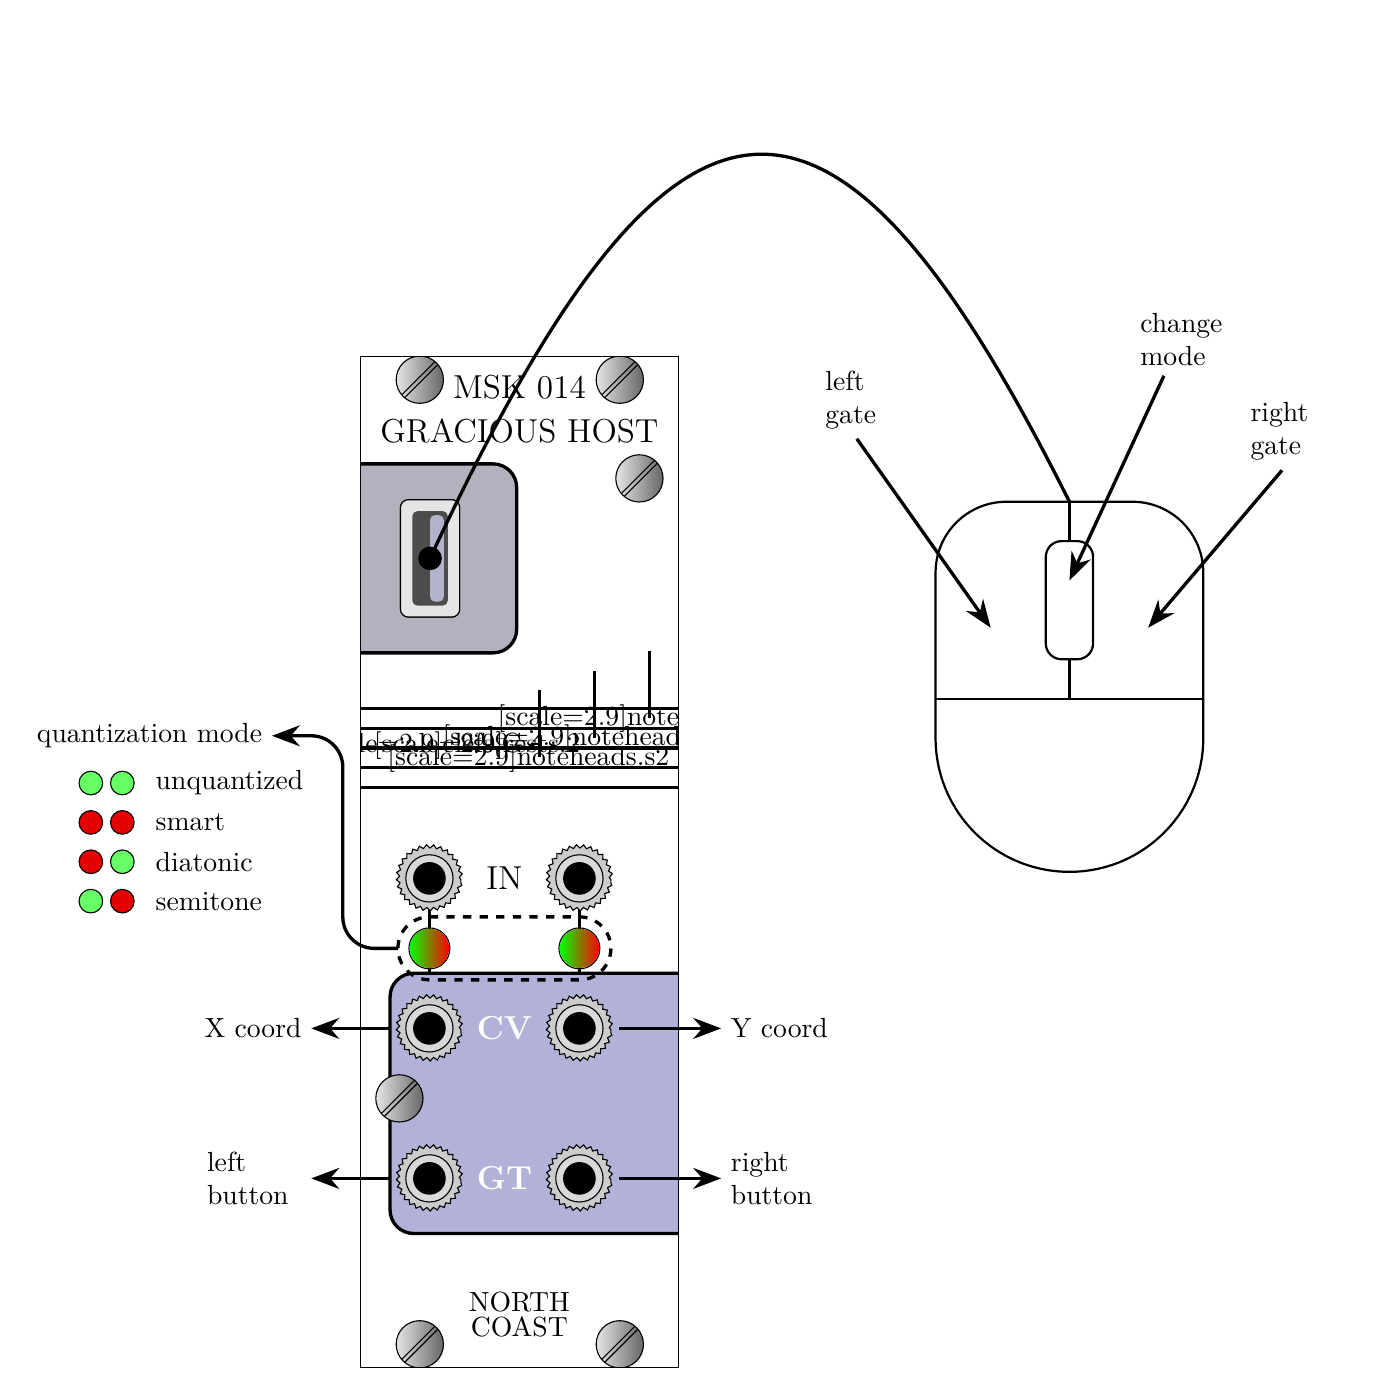
\begin{tikzpicture}
  \begin{scope}
    \setmainfont[Path={../../tsukurimashou/otf/},
      BoldFont={TsukurimashouBokukkoExtraBoldPS}]{TsukurimashouBokukkoDemiboldPS}%
    % start out defining coordinates
    \coordinate (o) at (0,0);
    \coordinate (llrh) at ($(o)+(7.50mm,3.00mm)$) {};
    \coordinate (ulrh) at ($(o)+(7.50mm,125.50mm)$) {};
    \coordinate (lrrh) at ($(o)+(32.90mm,3.00mm)$) {};
    \coordinate (urrh) at ($(o)+(32.90mm,125.50mm)$) {};
    \coordinate (lbh) at ($(o)+(4.91mm,34.23mm)$) {};
    \coordinate (ubh) at ($(o)+(35.39mm,112.97mm)$) {};
    \coordinate (j1) at ($(o)+(8.72mm,62.17mm)$) {};
    \coordinate (j2) at ($(o)+(27.77mm,62.17mm)$) {};
    \coordinate (j3) at ($(o)+(8.72mm,43.12mm)$) {};
    \coordinate (j4) at ($(o)+(27.77mm,43.12mm)$) {};
    \coordinate (j5) at ($(o)+(8.72mm,24.07mm)$) {};
    \coordinate (j6) at ($(o)+(27.77mm,24.07mm)$) {};
    \coordinate (d5) at ($(o)+(8.72mm,53.28mm)$) {};
    \coordinate (d6) at ($(o)+(27.77mm,53.28mm)$) {};
    \coordinate (j11) at ($(o)+(8.80mm,102.81mm)$) {};
%
    \coordinate (cpn) at ($(o)+(20.15mm,128.50mm)$) {};
    \coordinate (cps) at ($(o)+(20.15mm,0mm)$) {};
    \coordinate (cpe) at ($(o)+(40.30mm,64.25mm)$) {};
    \coordinate (cpw) at ($(o)+(0mm,64.25mm)$) {};
%
    % background
    \draw[fill=white] (o) rectangle (40.30mm,128.50mm);
    \clip (o) rectangle (40.30mm,128.50mm);
  %
    \draw[very thick,black,fill=blue!15!black!30!white,rounded corners=3.0mm]
      ($(j11)+(-15mm,-12mm)$) rectangle ($(j11)+(11mm,12mm)$);
    \draw[very thick,black] (j1) -- (j3);
    \draw[very thick,black] (j2) -- (j4);
    \draw[very thick,black,fill=blue!50!black!30!white,rounded corners=3.0mm]
      ($(j5)+(-5mm,-7mm)$) rectangle ($(j4-|cpe)+(5mm,7mm)$);
    \node at ($(j1)!0.5!(j2)$) {\large IN};
    \node[white] at ($(j3)!0.5!(j4)$) {\large\textbf{CV}};
    \node[white] at ($(j5)!0.5!(j6)$) {\large\textbf{GT}};
  %
    \coordinate (sref) at ($(j1)!0.53!(j11)$) {};
    \coordinate (nref) at ($(sref)+(9.525mm,-20.32mm)$) {};
    \draw[very thick] ($(sref-|cpw)$)
      -- ($(sref-|cpe)$);
    \draw[very thick] ($(sref-|cpw)+(0,-2.5mm)$)
      -- ($(sref-|cpe)+(0,-2.5mm)$);
    \draw[very thick] ($(sref-|cpw)+(0,-5mm)$)
      -- ($(sref-|cpe)+(0,-5mm)$);
    \draw[very thick] ($(sref-|cpw)+(0,-7.5mm)$)
      -- ($(sref-|cpe)+(0,-7.5mm)$);
    \draw[very thick] ($(sref-|cpw)+(0,-10mm)$)
      -- ($(sref-|cpe)+(0,-10mm)$);
    \node at ($(nref)+(-11.0mm,15.62mm)$)
      {\lilyGlyph[scale=2.9]{clefs.G}};
    \node at ($(nref)+(-3.5mm,15.62mm)$)
      {\lilyGlyph[scale=2.9]{rests.2}};
    \foreach \x/\y in {3.00/0.05,10.00/2.55,17.00/5.05} {
      \node at ($(nref)+(\x mm,14mm+\y mm)$)
        {\lilyGlyph[scale=2.9]{noteheads.s2}};
      \draw[very thick]
        ($(nref)+(\x mm+1.4mm,14.1mm+\y mm)$) -- ++(0,8.5mm);
    }
  %
    \node at ($(cpn)+(0.0mm,-4.0mm)$) {\large MSK 014};
    \node at ($(cpn)+(0.0mm,-9.5mm)$) {\large GRACIOUS HOST};
    \node at ($(cps)+(0.0mm,8.5mm)$)
      {\parbox{0.9in}{\linespread{0.75}\selectfont\center NORTH COAST}};
%
    % panel-to-rails mounting holes, 3.2mm holes to clear M3 machine screw
    \draw (llrh) circle[radius=1.60mm];
    \draw (ulrh) circle[radius=1.60mm];
    \draw (lrrh) circle[radius=1.60mm];
    \draw (urrh) circle[radius=1.60mm];
    % board-to-panel mounting holes, to clear M3 machine screw
    \draw (lbh) circle[radius=1.60mm];
    \draw (ubh) circle[radius=1.60mm];
    % six jacks with M6 threads, 6.3mm holes
    \draw (j1) circle[radius=3.15mm];
    \draw (j2) circle[radius=3.15mm];
    \draw (j3) circle[radius=3.15mm];
    \draw (j4) circle[radius=3.15mm];
    \draw (j5) circle[radius=3.15mm];
    \draw (j6) circle[radius=3.15mm];
    % two LEDs, 5.20mm holes
    \draw (d5) circle[radius=2.60mm];
    \draw (d6) circle[radius=2.60mm];
    % rectangular hole for USB A connector
    \draw[rounded corners=1mm]
      ($(j11)+(-3.76mm,-7.45mm)$) rectangle ($(j11)+(3.76mm,7.45mm)$);
%
    % machine screws with 6mm heads
    \foreach \screwname in {llrh,ulrh,lrrh,urrh,lbh,ubh} {
      \path[draw=black,shading=ball,
        left color=black!10!white,right color=black!60!white]
        (\screwname) circle[radius=3mm];
      \draw ($(\screwname)+(50:3.0mm)$)--($(\screwname)+(220:3.0mm)$);
      \draw ($(\screwname)+(40:3.0mm)$)--($(\screwname)+(230:3.0mm)$);
    }
    % jacks with knurled nuts
    \foreach \jackname in {j1,j2,j3,j4,j5,j6} {
      \path[draw=black,fill=black!20!white,
        decorate,decoration={snake,amplitude=0.6,segment length=2.5}]
        ($(\jackname)+(0,-0.15mm)$) circle[radius=4mm];
      \path[draw=black,fill=black!15!white] (\jackname) circle[radius=3mm];
      \path[draw=black,fill=black] (\jackname) circle[radius=2mm];
    }
    % LEDs with red/green gradient
    \foreach \ledname in {d5,d6} {
      \path[shading=ball,left color=green,right color=red]
        (\ledname) circle[radius=2.50mm];
    }
    % mock up USB connector
    \draw[rounded corners=1mm,fill=black!10!white]
      ($(j11)+(-3.76mm,-7.45mm)$) rectangle ($(j11)+(3.76mm,7.45mm)$);
    \fill[rounded corners=0.64mm,fill=black!70!white]
      ($(j11)+(-2.25mm,-6.00mm)$) rectangle ($(j11)+(2.25mm,6.00mm)$);
    \fill[rounded corners=0.64mm,fill=blue!35!black!30!white]
      ($(j11)+(0,-5.50mm)$) rectangle ($(j11)+(1.75mm,5.50mm)$);
  \end{scope}
  \draw (o) rectangle (40.30mm,128.50mm);
%
  \coordinate (mtab) at ($(d5)+(-20mm,27mm)$) {};
  \draw[very thick,{Stealth[scale=1.2]}-,rounded corners=4mm]
    (mtab) -- ($(d5|-mtab)+(-11mm,0mm)$) --
    ($(d5)+(-11mm,0)$) -- ($(d5)+(-4mm,0)$);
  \draw[rounded corners=4mm,very thick,dashed]
    ($(d5)+(-4mm,-4mm)$) rectangle ($(d6)+(4mm,4mm)$);
  \draw[very thick,{Stealth[scale=1.2]}-]
    ($(j3)+(-15mm,0)$) -- ($(j3)+(-5mm,0)$);
  \draw[very thick,{Stealth[scale=1.2]}-]
    ($(j4)+(18mm,0)$) -- ($(j4)+(5mm,0)$);
  \draw[very thick,{Stealth[scale=1.2]}-]
    ($(j5)+(-15mm,0)$) -- ($(j5)+(-5mm,0)$);
  \draw[very thick,{Stealth[scale=1.2]}-]
    ($(j6)+(18mm,0)$) -- ($(j6)+(5mm,0)$);
%
  \node[anchor=east] at (mtab) {quantization mode};
  \node[anchor=east] at ($(j3)+(-15mm,0)$) {X coord};
  \node[anchor=west] at ($(j4)+(18mm,0)$) {Y coord};
  \node[anchor=east] at ($(j5)+(-15mm,0)$)
    {\parbox{12mm}{left button}};
  \node[anchor=west] at ($(j6)+(18mm,0)$)
    {\parbox{12mm}{right button}};
%
  \path[draw,fill=green!60!white] ($(mtab)+(-23mm,-6mm)$)
    circle[radius=1.50mm];
  \path[draw,fill=green!60!white] ($(mtab)+(-19mm,-6mm)$)
    circle[radius=1.50mm];
  \node[anchor=west] at ($(mtab)+(-16mm,-6mm)$)
    {unquantized};
%
  \path[draw,fill=red!90!black] ($(mtab)+(-23mm,-11mm)$)
    circle[radius=1.50mm];
  \path[draw,fill=red!90!black] ($(mtab)+(-19mm,-11mm)$)
    circle[radius=1.50mm];
  \node[anchor=west] at ($(mtab)+(-16mm,-11mm)$)
    {smart};
%
  \path[draw,fill=red!90!black] ($(mtab)+(-23mm,-16mm)$)
    circle[radius=1.50mm];
  \path[draw,fill=green!60!white] ($(mtab)+(-19mm,-16mm)$)
    circle[radius=1.50mm];
  \node[anchor=west] at ($(mtab)+(-16mm,-16mm)$)
    {diatonic};
%
  \path[draw,fill=green!60!white] ($(mtab)+(-23mm,-21mm)$)
    circle[radius=1.50mm];
  \path[draw,fill=red!90!black] ($(mtab)+(-19mm,-21mm)$)
    circle[radius=1.50mm];
  \node[anchor=west] at ($(mtab)+(-16mm,-21mm)$)
    {semitone};
%
  \coordinate (mouse) at ($(o)+(90mm,110mm)$) {};
  \coordinate (arctop) at ($(o)+(50mm,170mm)$) {};
  \fill (j11) circle[radius=1.50mm];
  \draw[very thick] (j11)
    ..controls ($(arctop)+(-10mm,0)$) and ($(arctop)+(10mm,0)$)..
    (mouse);
  \path[thick,draw,fill=white]
    ($(mouse)+(-17mm,-9mm)$)
      arc[start angle=180,end angle=90,radius=9mm] --
    ($(mouse)+(-8mm,0mm)$) -- ($(mouse)+(8mm,0mm)$)
      arc[start angle=90,end angle=0,radius=9mm] --
    ($(mouse)+(17mm,-30mm)$)
      arc[start angle=0,end angle=-180,radius=17mm]
    --cycle;
  \draw[thick] ($(mouse)+(-17mm,-25mm)$) -- ($(mouse)+(17mm,-25mm)$);
  \draw[thick] (mouse) -- ($(mouse)+(0mm,-25mm)$);
  \draw[thick,fill=white,rounded corners=2mm]
    ($(mouse)+(-3mm,-20mm)$) rectangle ($(mouse)+(3mm,-5mm)$);
%
  \draw[very thick,{Stealth[scale=1.2]}-]
    ($(mouse)+(-10mm,-16mm)$) -- ($(mouse)+(-27mm,8mm)$);
  \draw[very thick,{Stealth[scale=1.2]}-]
    ($(mouse)+(10mm,-16mm)$) -- ($(mouse)+(27mm,4mm)$);
  \draw[very thick,{Stealth[scale=1.2]}-]
    ($(mouse)+(0mm,-10mm)$) -- ($(mouse)+(12mm,16mm)$);
%
  \node[anchor=south] at ($(mouse)+(-25mm,8mm)$) {\parbox{12mm}{left gate}};
  \node[anchor=south] at ($(mouse)+(29mm,4mm)$) {\parbox{12mm}{right gate}};
  \node[anchor=south] at ($(mouse)+(15mm,16mm)$) {\parbox{12mm}{change mode}};
\end{tikzpicture}\par}
\caption{Mouse interface functions.}\label{fig:mouse-conn}
\end{figure*}

The standardization of USB mice is much like that of typing keyboards:  the
relevant standard includes a very complicated protocol and a simple one, and
most implementors only use the simple one.  In technical terms, the Gracious
Host supports the ``boot mouse'' protocol, for USB devices that expose an
interface descriptor of class 3, subclass 1, protocol 2.  Nearly all
commonly-available USB mice can operate under this protocol.

The basic function with a mouse attached is that the left and right mouse
buttons send gates (to the Gracious Host's digital outputs) and the X and Y
coordinates of mouse motion control the analog CV outputs.  The middle
button (or wheel, when clicked) cycles between the quantization modes below;
and the colours of the LEDs (which light up on button presses) indicate the
current mode.

\begin{itemize}
  \item Unquantized (both LEDs green; default on startup) -- CV outputs
    directly reflect the current X and Y coordinates.
  \item Smart quantize (both LEDs red) -- CV outputs are quantized to a
    diatonic scale that attempts to automatically follow the notes you play. 
    Play the fourth of the (major) scale three times without playing the
    seventh and it will shift to the subdominant key; play the seventh three
    times without playing the fourth, and it will shift to the dominant.  In
    practice, this allows for free improvisation with the somewhat clumsy
    mouse control, while keeping everything more or less sounding like it is
    in tune.
  \item Quantize to fixed scale (left LED red, right green) -- CV outputs
    are quantized to a fixed diatonic scale (C major or A minor, if 0V
    output is considered to be C).
  \item Quantize to semitones (left LED green, right red) -- CV outputs are
    quantized to V/oct semitones, that is, round multiples of $1/12$ of a
    volt.
\end{itemize}

In the quantization modes, the CVs are quantized only while the button is
held and the gate is high; otherwise they are unquantized.  That way, it is
convenient to build a patch where one voltage is quantized pitch and the
other is something like filter cutoff not meant to be quantized; to control
the patch as intended, just don't press the button on the unquantized side.

The input jacks are not used in mouse mode, and (because the USB boot mouse
protocol does not specify this) the mouse wheel's scrolling
function, other than clicking it, has no consistent interpretation.

% $Id: warnings.tex 7623 2020-03-28 18:56:01Z mskala $

%
% MSK 013 safety and other warnings
% Copyright (C) 2020  Matthew Skala
%
% This program is free software: you can redistribute it and/or modify
% it under the terms of the GNU General Public License as published by
% the Free Software Foundation, version 3.
%
% This program is distributed in the hope that it will be useful,
% but WITHOUT ANY WARRANTY; without even the implied warranty of
% MERCHANTABILITY or FITNESS FOR A PARTICULAR PURPOSE.  See the
% GNU General Public License for more details.
%
% You should have received a copy of the GNU General Public License
% along with this program.  If not, see <http://www.gnu.org/licenses/>.
%
% Matthew Skala
% https://northcoastsynthesis.com/
% mskala@northcoastsynthesis.com
%

\chapter{Safety and other warnings}

Ask an adult to help you.

North Coast Synthesis Ltd.\ does not offer warranties or technical support
on anything we did not build and sell.  That applies both to modules built
by you or others from the kits we sell, and to fully-assembled modules that
might be built by others using our plans.  Especially note that because we
publish detailed plans and we permit third parties to build and sell modules
using our plans subject to the relevant license terms, it is reasonable to
expect that there will be modules on the new and used markets closely
resembling ours but not built and sold by us.  We may be able to help in
authenticating a module of unknown provenance; contact us if you have
questions of this nature.

For new modules purchased through a reseller, warranty and technical support
issues should be taken to the reseller \emph{first}.  Resellers buy modules
from North Coast at a significant discount, allowing them to resell the
modules at a profit, and part of the way they earn that is by taking
responsibility for supporting their own customers.

We also sell our products to hobbyists who enjoy tinkering with and
customizing electronic equipment.  Modules like ours, even if originally
built by us, may be quite likely to contain third-party ``mods,'' added or
deleted features, or otherwise differ from the standard specifications of
our assembled modules when new.  Be aware of this possibility when you buy a
used module.

Soldering irons are very hot.

Solder splashes and cut-off bits of component leads can fly a greater
distance and are harder to clean up than you might expect.  Spread out some
newspapers or similar to catch them, and wear eye protection.

Lead solder is toxic, as are some fluxes used with lead-free solder.  Do not
eat, drink, smoke, pick your nose, or engage in sexual activity while using
solder, and wash your hands when you are done using it.

Solder flux fumes are toxic, \emph{especially} from lead-free solder
because of its higher working temperature.  Use appropriate ventilation.

Some lead-free solder alloys produce joints that look ``cold''
(i.e.\ defective) even when they are correctly made.  This effect can be
especially distressing to those of us who learned soldering with lead solder
and then switched to lead-free.  Learn the behaviour of whatever alloy you  
are using, and then trust your skills.

Water-soluble solder flux must be washed off promptly (within less than an
hour of application) because if left in place it will corrode the metal. 
Solder with water-soluble flux should not be used with stranded wire because
it is nearly impossible to remove from between the strands.

Residue from traditional rosin-based solder flux can result in undesired
leakage currents that may affect high-impedance circuits.  This module does
not use any extremely high impedances, but small leakage currents could
possibly reduce its accuracy.  If your soldering leaves a lot of such
residue then it might be advisable to clean that off.

Voltage and current levels in some synthesizer circuits may be dangerous.

Do not attempt to make solder flow through the board and form fillets on
both sides of every joint.  Some soldering tutorials claim that that is
desirable or even mandatory, it does look nicer, and it may happen naturally
when the conditions are good and the leads happen to be small in relation to
the holes.  But with large wire leads that just fit in the holes, when the
holes are connected to the ground plane (even through thermal reliefs), on
some harder-to-wet lead finishes, with lead-free solder, and so on, you may
only end up dumping excessive heat into the joint and damaging the
components while you fuss over perfect fillets.  A well-made solder joint
that just covers the pad and makes good contact to the lead on one side of
the board, is good enough.

Building your own electronic equipment is seldom cheaper than buying
equivalent commercial products, due to commercial economies of scale from
which you as small-scale home builder cannot benefit.  If you think getting
into DIY construction is a way to save money, you will probably be
disappointed.

% $Id: bom.tex 8166 2020-09-17 19:18:02Z mskala $

%
% MSK 014 bill of materials
% Copyright (C) 2022  Matthew Skala
%
% This program is free software: you can redistribute it and/or modify
% it under the terms of the GNU General Public License as published by
% the Free Software Foundation, version 3.
%
% This program is distributed in the hope that it will be useful,
% but WITHOUT ANY WARRANTY; without even the implied warranty of
% MERCHANTABILITY or FITNESS FOR A PARTICULAR PURPOSE.  See the
% GNU General Public License for more details.
%
% You should have received a copy of the GNU General Public License
% along with this program.  If not, see <http://www.gnu.org/licenses/>.
%
% Matthew Skala
% https://northcoastsynthesis.com/
% mskala@northcoastsynthesis.com
%

\onecolumn
\chapter{Bill of materials}\label{cha:bom}

{\centering
\fbox{This table is not a substitute for the text instructions.}

\begin{longtable}{rp{1.4in}cp{2.9in}}
  \textbf{Qty} & \textbf{Ref} & \textbf{Value/Part No.} & \\ \hline \endhead
\input{bomdata.tex}
\end{longtable}\par}

Fixed resistors should be 1\%\ metal film throughout.
RoHS-certified zinc-plated steel hardware is recommended, not stainless
steel because of galvanic-corrosion incompatibility with aluminum parts.

Also needed:  solder and related supplies, two PCBs, three configuration
jumpers, front panel, 16-pin Eurorack power cable, etc.

Optional parts that may be added for development (not included in kits):

{\centering
\begin{longtable}{rp{1.4in}cp{2.9in}}
  \textbf{Qty} & \textbf{Ref} & \textbf{Value/Part No.} & \\ \hline \endhead
  1 & \raggedright P4 &  & male single-row header, 6 pins at 0.1$''$ \\
  1 & \raggedright U7 & 7805 & +5V regulator in TO-220 package \\
\end{longtable}\par}

In some builds and kits the LM224 op amp chips may actually be LM224A.

\twocolumn

% $Id: board2.tex 9464 2021-10-14 16:51:12Z mskala $

%
% MSK 009 Board 2 build instructions
% Copyright (C) 2018  Matthew Skala
%
% This program is free software: you can redistribute it and/or modify
% it under the terms of the GNU General Public License as published by
% the Free Software Foundation, version 3.
%
% This program is distributed in the hope that it will be useful,
% but WITHOUT ANY WARRANTY; without even the implied warranty of
% MERCHANTABILITY or FITNESS FOR A PARTICULAR PURPOSE.  See the
% GNU General Public License for more details.
%
% You should have received a copy of the GNU General Public License
% along with this program.  If not, see <http://www.gnu.org/licenses/>.
%
% Matthew Skala
% https://northcoastsynthesis.com/
% mskala@northcoastsynthesis.com
%

\chapter{Building Board 2}

The recommended order for building this module is to assemble Board 2, the
one further from the front panel, first.  That will make it easier to get
all the physical positioning right for the components that bridge between
the boards or pass through the panel.

Note that although I'm describing a separate step for each component value,
and that's how I built my prototype so as to have plenty of photo
opportunities, if you are reasonably confident about your skills you may
find it easier to populate all or most of the board (i.e.\ put the
components in place) and then solder them in a single step.  Except where
noted, the order in which you add components does not matter much.

\section{Preliminaries}

Count out the right number of everything according to the bill of materials. 
There is an abbreviated BOM for Board~2, excluding a few items that will be
added when combining this board with Board~1, in Table~\ref{tab:b2bom}.

\nopagebreak
\noindent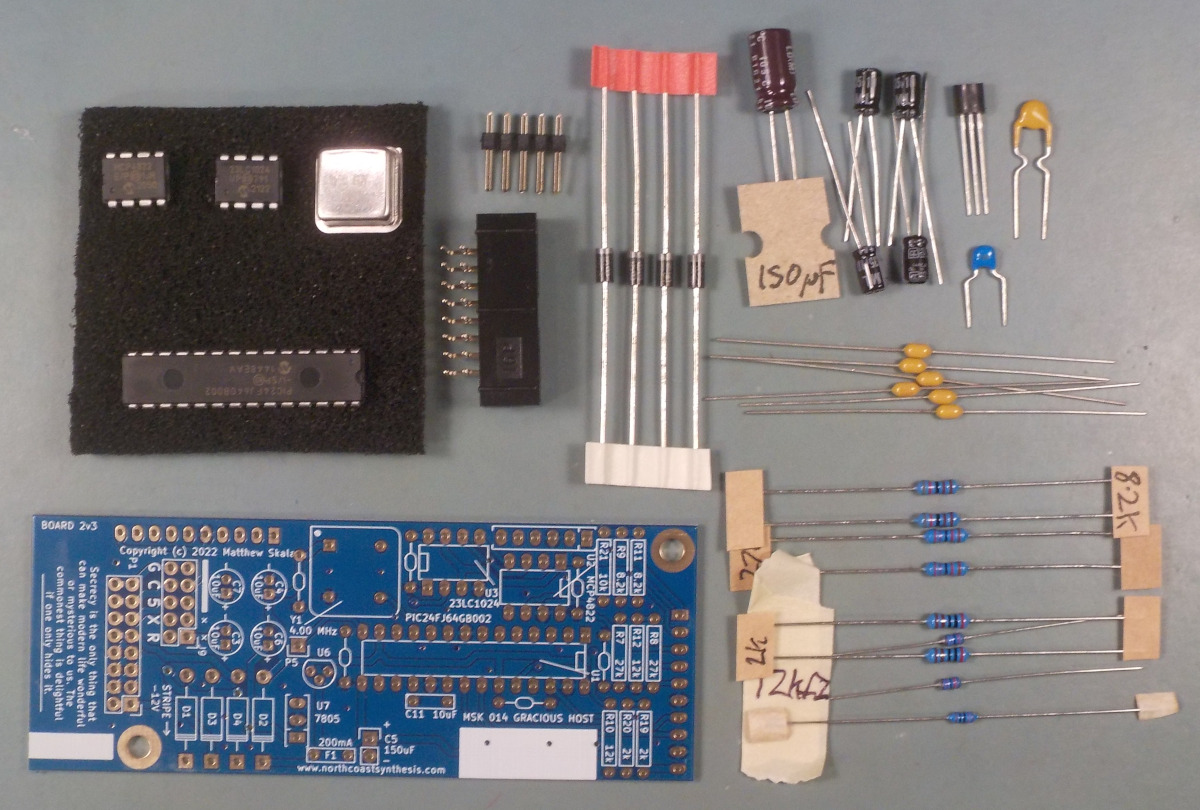
\includegraphics[width=\linewidth]{board2-parts.jpg}

There are two trimmers to be installed on this board.  Before
installing them, use an ohmmeter to adjust each one to 50\% of its range. 
Measure the resistance along the track, then measure the resistance from the
wiper to one end and adjust to make the wiper half the total track
resistance.  This need not be exact, but having them start near their
midpoints will help with adjustment later,
by reducing issues with interaction among the different settings.  With both
trimmers pre-set to 50\%, the module should basically work even if it is not
at its best, whereas if they are installed at extreme values instead, then
you may have trouble getting it up and running enough to adjust it more
accurately.

\begin{table*}
{\centering
\fbox{This table is not a substitute for the text instructions.}
\vspace{\baselineskip}

\begin{tabular}{rp{1.3in}cp{3in}}
  \textbf{Qty} & \textbf{Ref} & \textbf{Value/Part No.} & \\ \hline
\input{bomdata-2.tex}
\end{tabular}\par}
\caption{Bill of Materials for assembling Board~2.  Also needed is the PCB
itself.}\label{tab:b2bom}
\end{table*}

\section{Decoupling capacitors}

The four axial ceramic 0.1$\mu$F decoupling capacitors, C8 to C11, are shown
on the board by a special symbol without their reference designators.

\nopagebreak
\noindent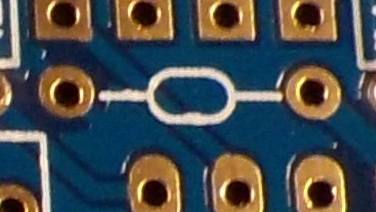
\includegraphics[width=\linewidth]{decoup-symbol.jpg}

Install these four capacitors where the symbol appears.  They are not
polarized and may be installed in either orientation.  These capacitors act
as filters for the power supplies to the op amp and OTA chips.  An MSK~009
kit should include six of these capacitors, and only four are used on this
board; save the remaining two for use on Board~1.

\nopagebreak
\noindent\includegraphics[width=\linewidth]{{cap-0.1u2}.jpg}

\section{Fixed resistors}

Resistors are never polarized.  I like to install mine in a consistent
direction for cosmetic reasons, but this is electrically unnecessary.  In
this module, the fixed resistors are metal film 1\%\ type.  They usually
have blue bodies and four colour bands designating the value, plus a fifth
band for the tolerance.  The tolerance band is brown for 1\%, but note that
we may occasionally ship better-tolerance resistors in the kits than the
specifications require, if we are able to source them at a good price. 
Accordingly, I mention only the four value band colours for this type of
resistor; if you are using resistors with other codes, you are responsible
for knowing them.  Note that colour codes on metal film 1\% resistors are
often ambiguous (reading from one end or the other end may give two
different values, both plausible) and some of the colours are hard to
distinguish anyway.  If in doubt, always measure with an ohmmeter before
soldering the resistor in place.

Install the four 510$\Omega$ (green-brown-black-black) resistors R22, R23,
R32, and R33.  These resistors, with the 100k$\Omega$ ones added later, set
the signal levels at the inputs of the OTA chips.

\nopagebreak
\noindent\includegraphics[width=\linewidth]{{res-510}.jpg}

\pagebreak
Install the two 9.1k$\Omega$ (white-brown-black-brown) resistors R24 and
R34.  These limit the maximum control current for the OTAs.

\nopagebreak
\noindent\includegraphics[width=\linewidth]{{res-9.1k}.jpg}

Install the two 10k$\Omega$ (brown-black-black-red) resistors R25 and R35. 
These are feedback resistors for the current-to-voltage converters in the
filter core.

\nopagebreak
\noindent\includegraphics[width=\linewidth]{{res-10k}.jpg}

\pagebreak
Install the four 27k$\Omega$ (red-violet-black-red) resistors R21, R26, R31, and R36. 
These are feedback resistors for the integrators (R26 and R36), and set the
current for the linearizing diodes in the LM13700 chips (R1 and R31).

\nopagebreak
\noindent\includegraphics[width=\linewidth]{{res-27k}.jpg}

Install the two 100k$\Omega$ (brown-black-black-orange) resistors R18 and
R28.  These resistors participate in setting the input levels for the OTA
chips.  A full kit contains seven resistors of this value; five should
remain for use on Board~1.

\nopagebreak
\noindent\includegraphics[width=\linewidth]{{res-100k2}.jpg}

Install the two 220k$\Omega$ (red-red-black-orange) resistors R19 and
R29.  These resistors set the adjustment ranges for the DC offset trimmers.
A full kit contains four
resistors of this value; save two for use on Board~1.

\nopagebreak
\noindent\includegraphics[width=\linewidth]{{res-220k2}.jpg}

\section{Semiconductors}

Install the two 1N5818 or SBA130 Schottky rectifier diodes D2 and D3.  These
are for reverse-voltage protection; they cut off power to the module when
the power plug is backwards.  They are polarized and it is important to
install them in the right direction.  Each diode is packaged inside a black
or dark grey plastic slug with a white or light grey stripe at one end; that
end is the \emph{cathode}.  The silkscreen markings on the board have a
corresponding stripe and the diodes should be installed with their stripes
matching the markings on the board.  The solder pads for the cathodes are
also square instead of round.  Installing these backwards means they will
have the opposite of the intended protective effect.

\nopagebreak
\noindent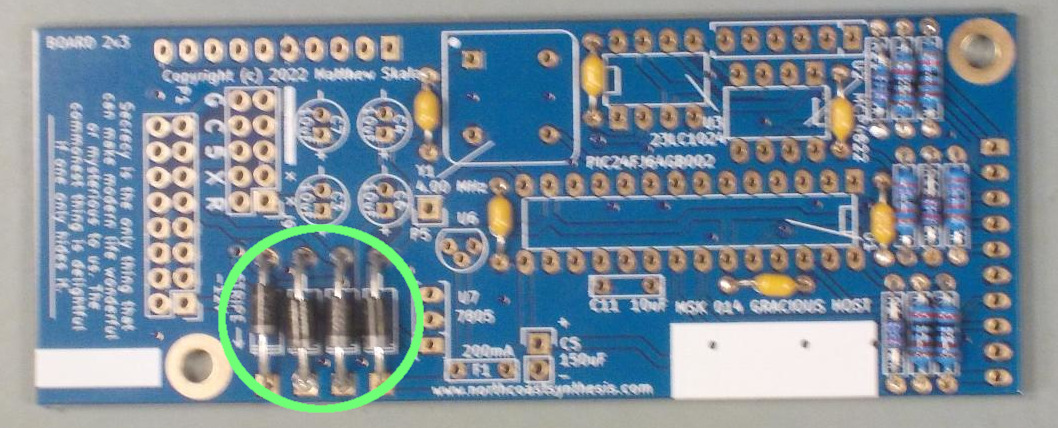
\includegraphics[width=\linewidth]{schottky.jpg}

Install the 14-pin DIP socket for the operational amplifier chip U2.  This
chip does most of the amplification in the filter core.  DIP sockets
themselves do not care which direction you install them, but it is
critically important that the chips installed in the sockets should be
installed in the right direction.  To help with that, the sockets will
probably be marked with notches at one end (indicating the end where Pin~1
and Pin~14 are located) and you should install the sockets so that the
notched ends match the notches shown on the PCB silkscreen.  The solder pad
for Pin~1 is also distinguished by being rectangular instead of rounded.

Installing DIP sockets without having them tilted at a funny angle can be
tricky.  I recommend inserting the socket in the board, taping it in place
on the component side with vinyl electrical tape or sticking it there with a
small blob of putty at each end, then soldering one pin on
one corner and checking that the socket is snug against the board before
soldering the other pins.  That way, if you accidentally solder the first
pin with the socket tilted, it will be easier to correct (only one pin to
desolder instead of all of them).

\nopagebreak
\noindent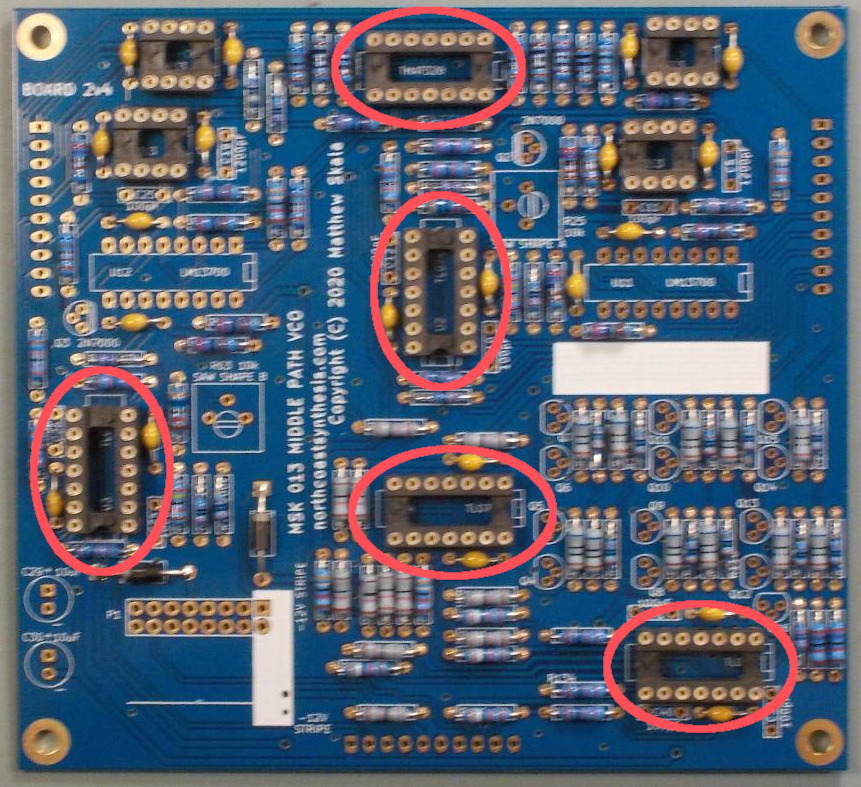
\includegraphics[width=\linewidth]{dip14-2.jpg}

If you somehow manage to solder an entire socket in backwards, don't try to
desolder it to turn it around.  Just leave it as it is and remember that
when you insert the chip, you must insert it so the chip matches the
markings on the \emph{board}, not the turned-around socket.

Install the 16-pin DIP socket for the OTA (operational transconductance
amplifier) chip U3.  This chip contains two current-controlled amplifiers,
which, by means of a frequency-dependent control current, tune the filter
core to the desired frequency.  See the general instructions regarding DIP
sockets above.

\nopagebreak
\noindent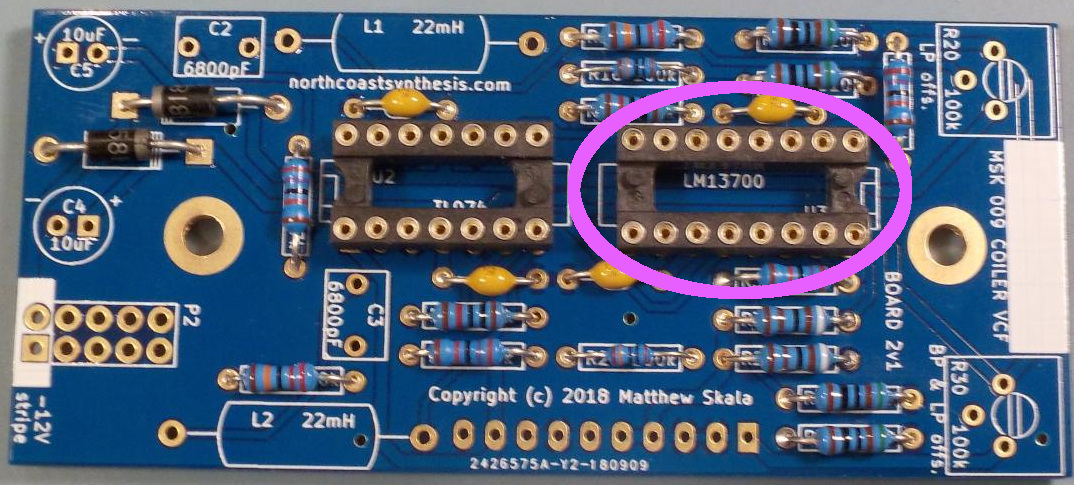
\includegraphics[width=\linewidth]{dip16.jpg}

\section{Electrolytic and film capacitors}

Install the two 6800pF film capacitors C2 and C3.  These are timing
components used in the integrators at low frequencies to complement the
inductors used at medium to high frequencies.  They are unpolarized
components and may be installed in either orientation.

The markings on film capacitors may vary depending on the manufacturer and
model.  These ones might be marked ``682'' (for 68 followed by two 0s number
of picofarads), ``6n8'' (for 6.8nF), or even ``0.0068'' (value in $\mu$F). 
However, these are the only film capacitors in the module, so confusion is
unlikely.

\nopagebreak
\noindent\includegraphics[width=\linewidth]{{cap-6800p}.jpg}

\pagebreak

Install the two 10$\mu$F electrolytic capacitors C4 and C5, which
filter the power supply for the module as a whole. 
These are polarized components and they may explode if installed backwards. 
Each one will be marked on its casing with a stripe and minus signs to
indicate the negative lead; the positive lead will probably also be longer. 
These clues should be matched with the markings on the PCB: plus and minus
symbols in the silkscreen and a square solder pad for the positive (long)
lead.

\nopagebreak
\noindent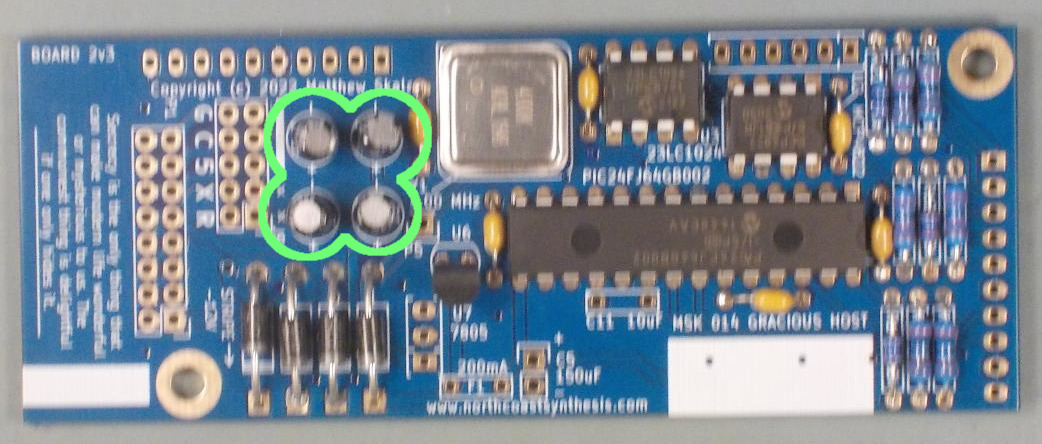
\includegraphics[width=\linewidth]{cap-10u.jpg}

\section{Trimmer potentiometers}

If you have not already set the trimmers to 50\%\ of their full scale value
as described under ``Preliminaries'' above, then do it now.

Trimmers usually are not washable, so if you plan to clean your boards by
full immersion in water or other solvent,
your last chance is now; future cleaning will have to
be done with a brush and some care to avoid letting liquid seep into the
trimmers.  Even now you should take some care with the DIP sockets, because
solvent can carry flux residue into them and form a varnish-like layer if
not carefully rinsed away.

Trimmers are not exactly polarized, but the three legs of each trimmer serve
different functions and need to be connected to the right holes.  The
physical arrangement of the legs and corresponding holes should make it
impossible to install the trimmers wrong way round.

Install the two 100k$\Omega$ trimmers R20 and R30.  These trimmers
are for compensating DC offsets in the filter core.

\nopagebreak
\noindent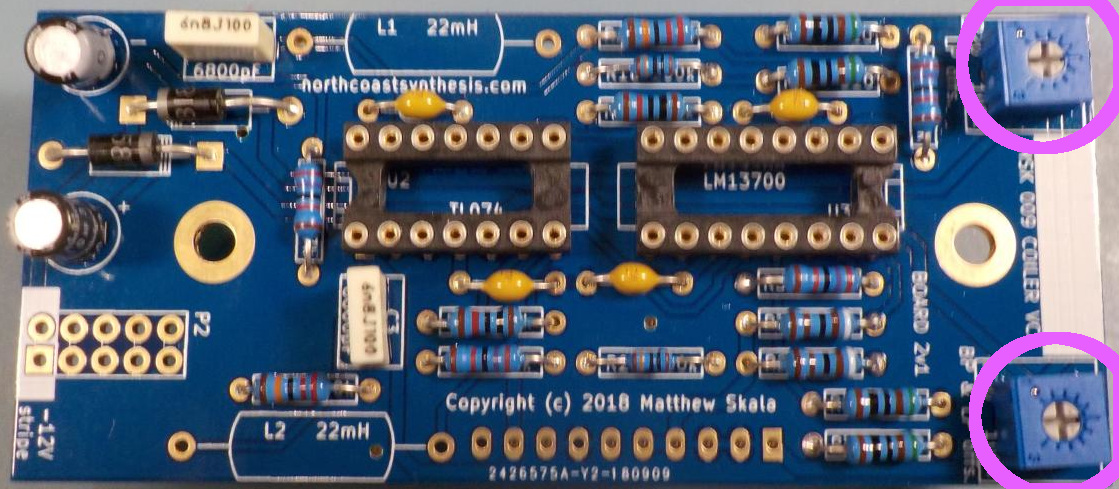
\includegraphics[width=\linewidth]{pot-100k2.jpg}

\pagebreak

\section{Inductors}

The two 22mH ferrite-bobbin inductors, that is, \emph{coils}, L1 and L2 give
this module its name.  Install them now.  They are the main timing
components in the filter core, serving at medium to high frequencies. 
Single inductors like these have no polarity and may be installed in either
direction; the situation is more complicated with transformers made of two
or more interacting inductors.

The inductors are delicate, especially in the area where the leads attach to
the bodies, because the windings that connect to the leads are made of very
fine wire.  The ferrite core material is also somewhat brittile.  It is
important not to bend the leads too close to the bodies.  There is some
extra space for the inductors on the circuit board to allow for a gentle
bend radius.

\nopagebreak
\noindent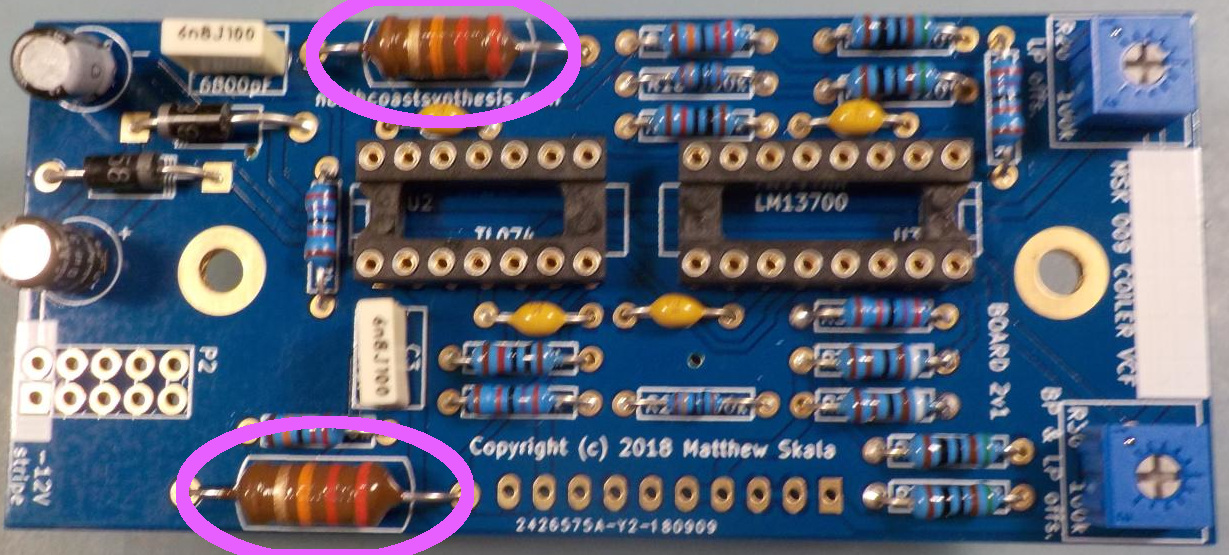
\includegraphics[width=\linewidth]{coils.jpg}

\section{Eurorack power connector}

Install the 2$\times$5-pin Eurorack power connector J2.  This connector is
not polarized in itself, although the connection it makes is polarized.  As
with the DIP sockets, you should be careful to get it installed snugly
against the board, not tilted at an angle.  Use tape or putty to
hold it in place, solder one pin, then check that it is straight before you
solder the other pins.

The six pins in the centre of the connector, that is all except the four
corner pins, are for grounding and they are all connected together on the
board.  Thus, if you accidentally form solder bridges among these six pins
while installing the connector, don't waste effort trying to remove them;
they will have no electrical effect.

\nopagebreak
\noindent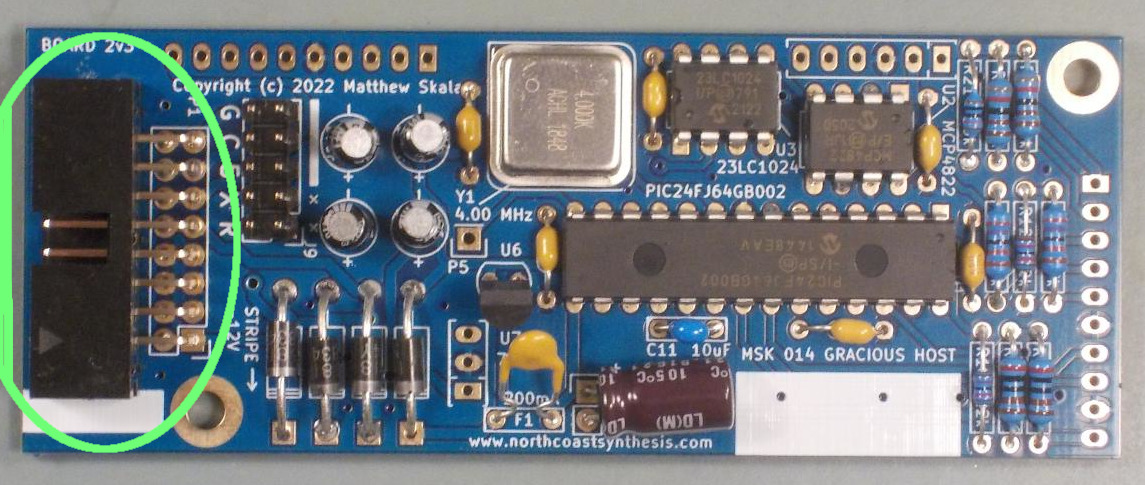
\includegraphics[width=\linewidth]{power.jpg}

In between completed boards is a good time to take a break.


% $Id: board1.tex 9375 2021-08-31 13:01:06Z mskala $

%
% MSK 007 Board 1 build instructions
% Copyright (C) 2017, 2020, 2021  Matthew Skala
%
% This program is free software: you can redistribute it and/or modify
% it under the terms of the GNU General Public License as published by
% the Free Software Foundation, version 3.
%
% This program is distributed in the hope that it will be useful,
% but WITHOUT ANY WARRANTY; without even the implied warranty of
% MERCHANTABILITY or FITNESS FOR A PARTICULAR PURPOSE.  See the
% GNU General Public License for more details.
%
% You should have received a copy of the GNU General Public License
% along with this program.  If not, see <http://www.gnu.org/licenses/>.
%
% Matthew Skala
% https://northcoastsynthesis.com/
% mskala@northcoastsynthesis.com
%

\chapter{Building Board 1}

Board~1 has components on both sides, which makes the order of assembly
important; installing the wrong components first may make it difficult to
safely maneuver the soldering iron to install later components without
damaging the already-installed components.  This chapter also includes
instructions on installing the connector on Board~2 that links it to
Board~1.

\section{Preliminaries}

Count out the right number of everything according to the bill of materials. 
There is an abbreviated BOM for Board~1, and the final assembly steps, in
Table~\ref{tab:b1bom}.  In addition to these things you will need your
assembled Boards~2 and~3 from the previous chapters, and the hardware
associated with them.

\noindent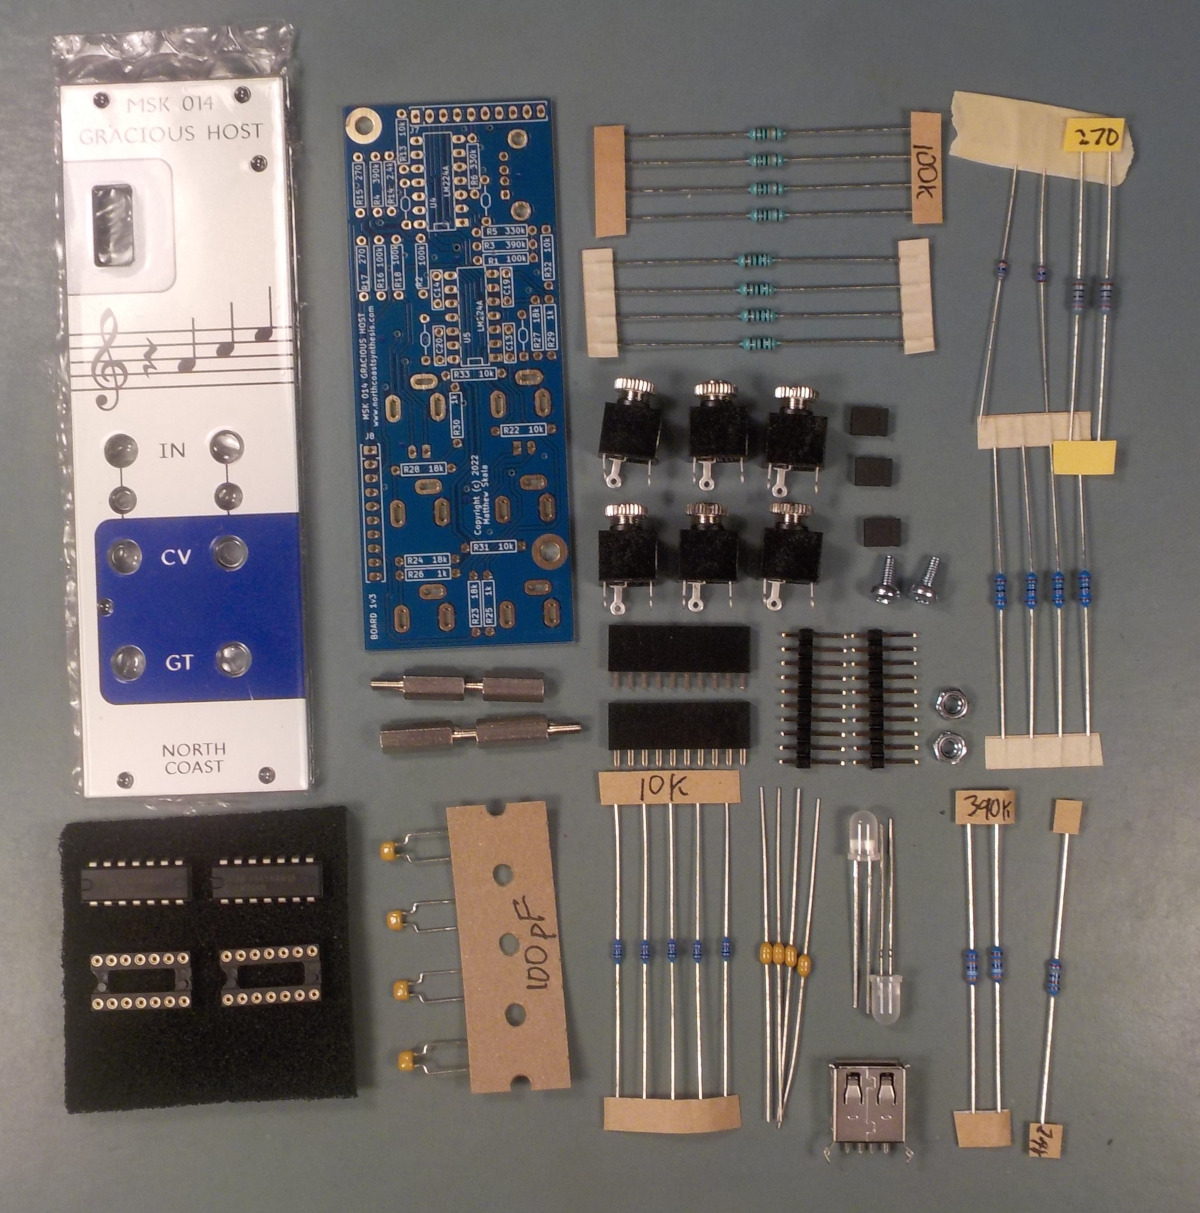
\includegraphics[width=\linewidth]{board1-parts.jpg}

There are two multiturn trimmers to be installed on this board.  Before
installing them, use an ohmmeter to adjust each one to 50\% of its range. 
Measure the resistance along the track, then measure the resistance from the
wiper to one end and adjust to make the wiper half the total track
resistance.  This need not be exact, but it will help with adjustment later,
by reducing issues with interaction among the different settings.  With all
trimmers pre-set to 50\%, the module should basically work even if it is not
at its best, whereas if many are installed at extreme values instead, then
you may have trouble getting it up and running enough to adjust it more
accurately.

\begin{table*}
{\centering
\fbox{This table is not a substitute for the text instructions.}
\vspace{\baselineskip}

\begin{tabular}{rp{1in}cp{3in}}
  \textbf{Qty} & \textbf{Ref} & \textbf{Value/Part No.} & \\ \hline
\input{bomdata-1.tex}
\end{tabular}\par}
\caption{Bill of Materials for Board~1.  Also needed:  knobs, a cable tie,
and module-to-rack mounting~hardware.}\label{tab:b1bom}
\end{table*}

\section{Some notes on knobs}

The first batch of knobs I ordered for North Coast products turned out to
have serious quality problems, specifically with the setscrews that hold the
knobs onto the potentiometer shafts.  Some of the screws had marginal
threads that would strip when the screw was tightened, and I ended up having
to do a bunch of extra testing and ship extra knobs to some customers to
replace any that might fail.  Later batches have also had issues, although
they're under better control now because the bad first batch served as a
warning to step up the testing procedures.  Starting with kits prepared in
August 2019, I switched to blue knobs with 100\%\ testing; in September
2020, I switched to a new manufacturer, and knobs that are a slightly darker
shade of blue.  Although all the knobs I ship in kits now have been tested
and passed at least twice, and should be fine to use, I am also shipping
spare setscrews in any kits with knobs from batches where a signficant
number of knobs failed testing.

Here are some things to be aware of as a kit builder.

\begin{itemize}
\item Some photos in these instructions were taken with the older grey
knobs, and some dealers may still have kits containing grey knobs in their
stock, but newer kits will have blue knobs.

\item Do not overtighten the setscrews when attaching the knobs!  The screw
should be tight enough to hold the knob onto the shaft, but there's no
advantage to making it tighter than that, and overtightening may risk
destroying the screw thread or damaging the drive slot.

\item If, despite my efforts to make sure no bad screws get sent to
customers, you still get a bad screw that cannot be tightened and no spare
for it, then please contact me.

\item If you want to source an exact replacement for the setscrew, it should
be an M3$\times$3mm flat-tip slotted setscrew, which is also sometimes
called a ``grub screw,'' made of RoHS-compliant brass (possibly by
exemption).  Stainless steel is fine too, and I may sometimes ship stainless
steel screws instead of brass if I can find a reliable source for them;
plain steel should not be used here for galvanic corrosion reasons. 
Hex-socket screws are fine if you have the driver for them, but I don't ship
those because I'm not sure all DIY builders do have the right driver.

\item Because it's a standard M3 thread, in a pinch it's possible to
substitute a plain M3 machine screw such as are commonly used with Eurorack
cases, although one of those would obviously look less nice.
\end{itemize}

\section{Fixed resistors}

Resistors are never polarized.  I like to install mine in a consistent
direction for cosmetic reasons, but this is electrically unnecessary.  In
this module, metal film 1\%\ resistors are recommended for all fixed-value
resistors.  These will usually have blue bodies and four colour bands
designating the value, plus a fifth band for the tolerance, brown in the
case of 1\%.  These are the resistors normally shipped in the
North Coast kits, but we may occasionally ship better-tolerance resistors (such
as 0.5\%) if we are able to source them at a good price. 
Accordingly, I mention only the four value band colours for this type of
resistor; if you are using resistors with other codes, you are responsible
for knowing them.  Note that colour codes on metal film 1\% resistors are
often ambiguous (reading from one end or the other end may give two
different values, both plausible) and some of the colours are hard to
distinguish anyway.  If in doubt, always measure with an ohmmeter before
soldering the resistor in place.

\pagebreak

Install the 1k$\Omega$ (brown-black-black-brown) resistor R80.  This
resistor limits the current that can flow on the module output, as well as
separating the output driver op amp and its stability capacitor from any
destabilizing capacitance that may be attached to the output (for instance,
from a long patch cable).  Do not confuse it with the other power-of-ten
resistor values (10k$\Omega$, 100k$\Omega$, and 1M$\Omega$).

\nopagebreak
\noindent\includegraphics[width=\linewidth]{{res-1.0k1}.jpg}

Install the two 2.7k$\Omega$ (red-violet-black-brown) resistors R72 and R76.
These resistors are used in the exponential converter, R72 as part of the
network that scales the control voltage and R76 to control voltage and
current at the output of the servo op amp.  Do not confuse them with the
27k$\Omega$ resistor, which has a similar colour code and is to be
mounted in a PCB footprint near that of R72.

\nopagebreak
\noindent\includegraphics[width=\linewidth]{{res-2.7k1}.jpg}

\pagebreak

Install the 3.3k$\Omega$ (orange-orange-black-brown) resistor R58.
This resistor is used in the linear voltage-to-current converter that
provides control current to the VCA section.

\nopagebreak
\noindent\includegraphics[width=\linewidth]{{res-3.3k1}.jpg}

Install the 5.6k$\Omega$ (green-blue-black-brown) resistor R60.
This resistor converts the exponential converter's output current back to a
voltage for broadcast to the five integrators.

\nopagebreak
\noindent\includegraphics[width=\linewidth]{{res-5.6k1}.jpg}

\pagebreak

Install the 10k$\Omega$ (brown-black-black-red) resistor R82.
This resistor sets the maximum attenuation of the VCA soft-clipping section. 
Do not confuse it with the other power-of-ten resistor values, nor the
11k$\Omega$ resistor.

\nopagebreak
\noindent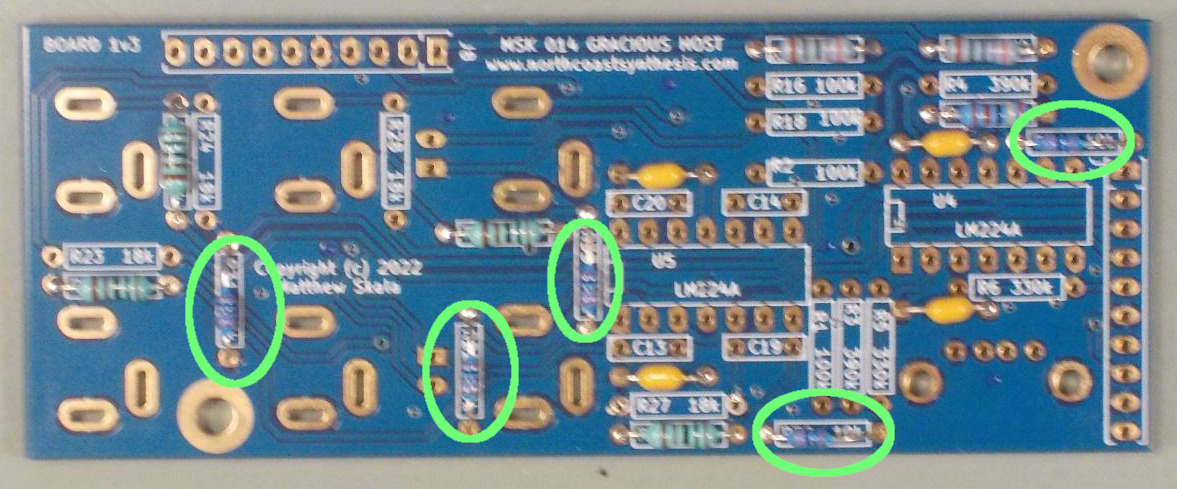
\includegraphics[width=\linewidth]{res-10k1.jpg}

Install the 11k$\Omega$ (brown-brown-black-red) resistor R67.
This resistor is part of the pitch control voltage scaling network.

\nopagebreak
\noindent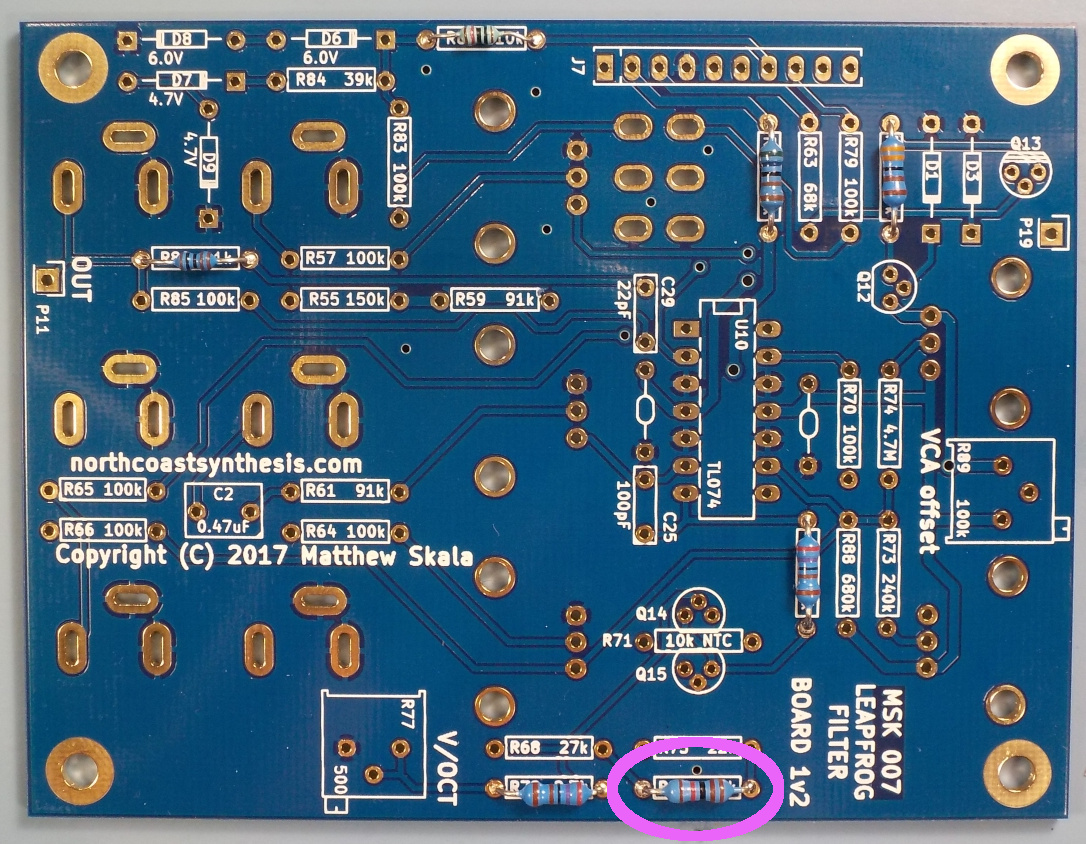
\includegraphics[width=\linewidth]{res-11k1.jpg}

\pagebreak

Install the 22k$\Omega$ (red-red-black-red) resistor R75.
This resistor sets the gain of the op amp in the control voltage scaling
network.

\nopagebreak
\noindent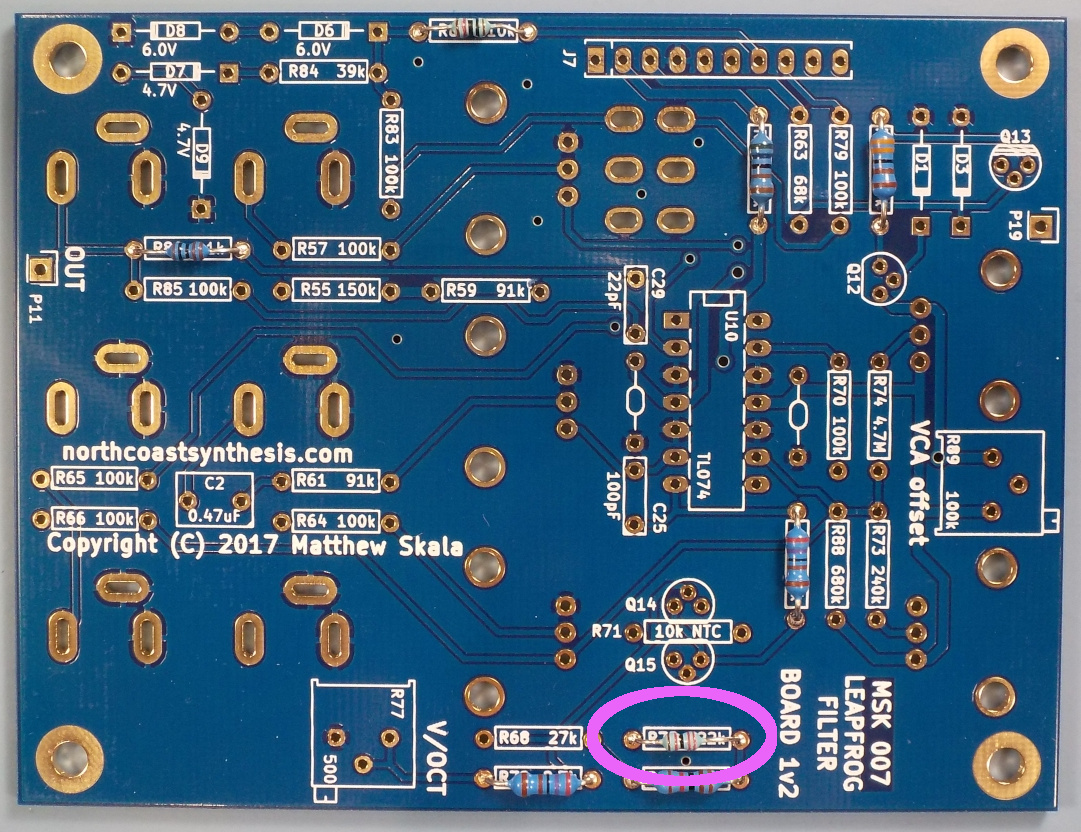
\includegraphics[width=\linewidth]{res-22k1.jpg}

Install the 27k$\Omega$ (red-violet-black-red) resistor R68.
This resistor is another part of the control voltage scaling network.

\nopagebreak
\noindent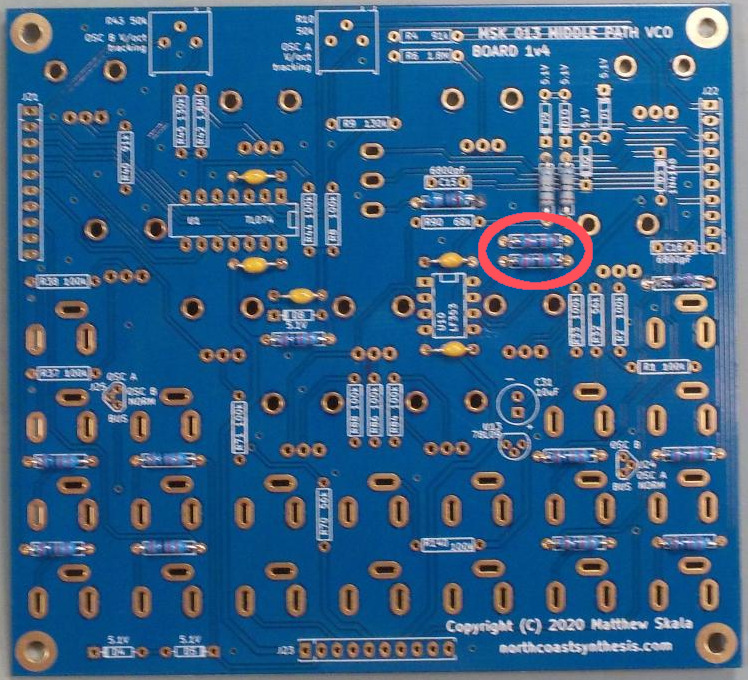
\includegraphics[width=\linewidth]{res-27k1.jpg}

\pagebreak

Install the 39k$\Omega$ (orange-white-black-red) resistor R84.
This resistor sets the mid-level attenuation of the VCA soft-clipping
circuit.

\nopagebreak
\noindent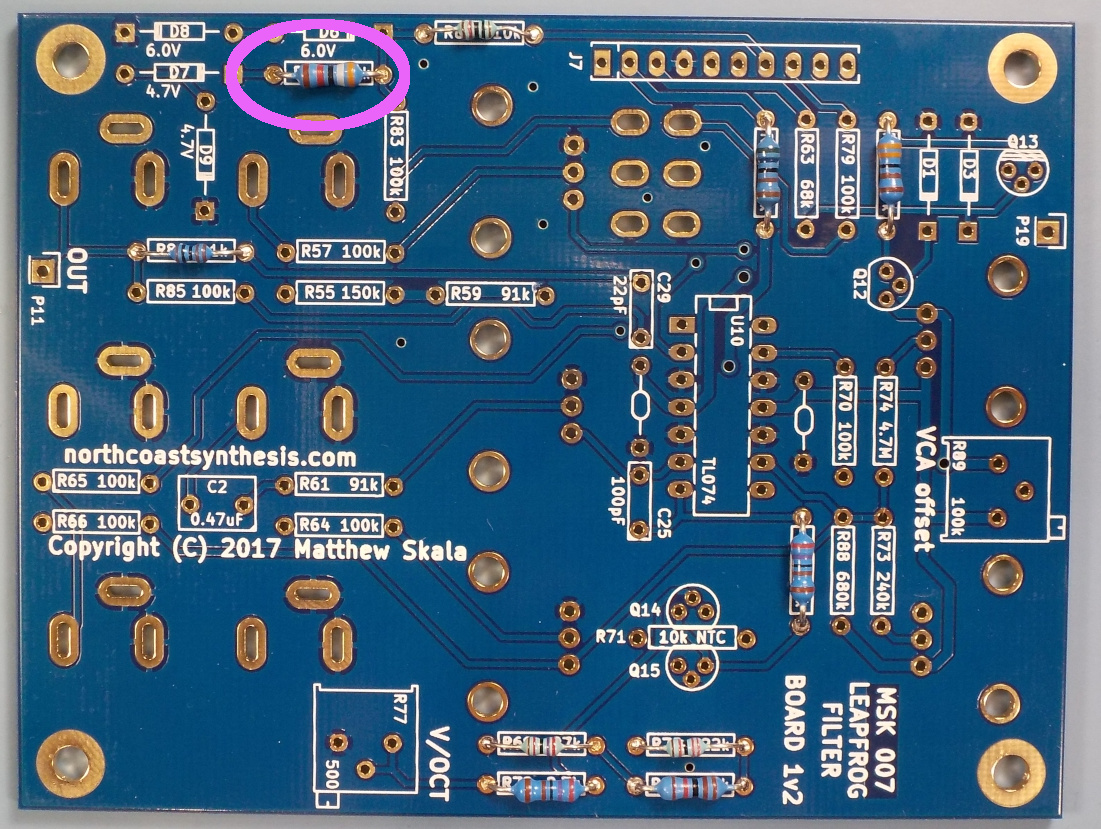
\includegraphics[width=\linewidth]{res-39k1.jpg}

Install the 68k$\Omega$ (blue-grey-black-red) resistor R63.
This resistor pulls down the base of the transistor Q13 to bring the VCA's
zero-gain point near 0V.  Do not confuse it with the 680k$\Omega$ resistor,
which has a similar colour code.

\nopagebreak
\noindent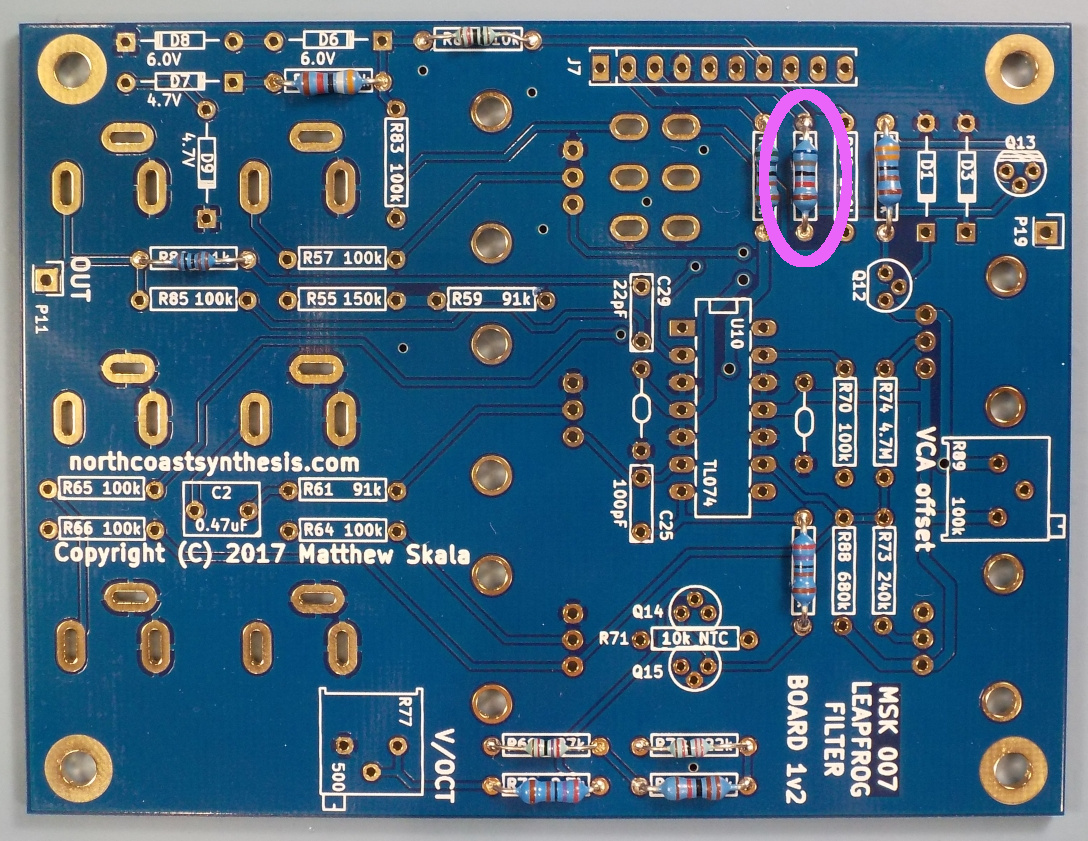
\includegraphics[width=\linewidth]{res-68k1.jpg}

\pagebreak

Install the two 91k$\Omega$ (white-brown-black-red) resistors R59 and R61. 
These two resistors set the reference current for the exponential converter,
and the maximum sensitivity of the linear FM input, respectively.

\nopagebreak
\noindent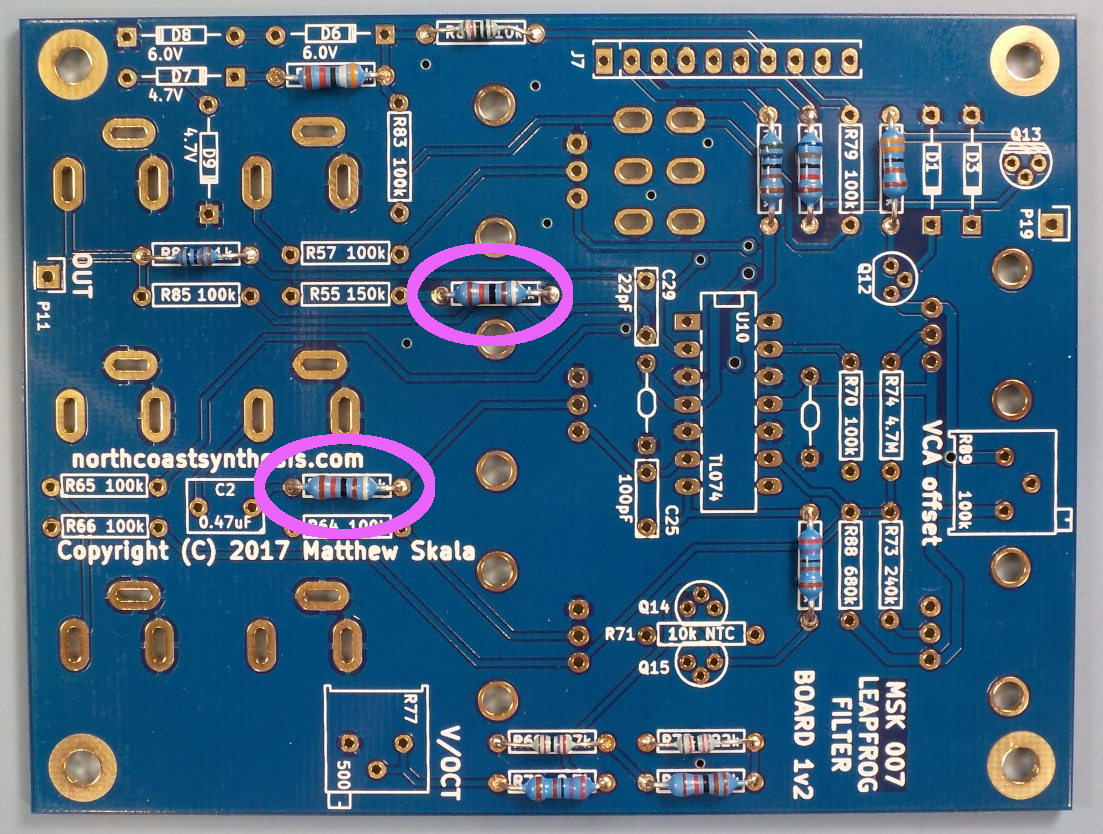
\includegraphics[width=\linewidth]{res-91k1.jpg}

Install the eight 100k$\Omega$ (brown-black-black-orange) resistors R57, R64
through R66, R70, R79, R83, and R85.
These resistors are used in multiple places throughout the input and output
circuits to either set input impedances to Eurorack standard, or set op amp
gain to negative unity by balancing against an input resistor.

\nopagebreak
\noindent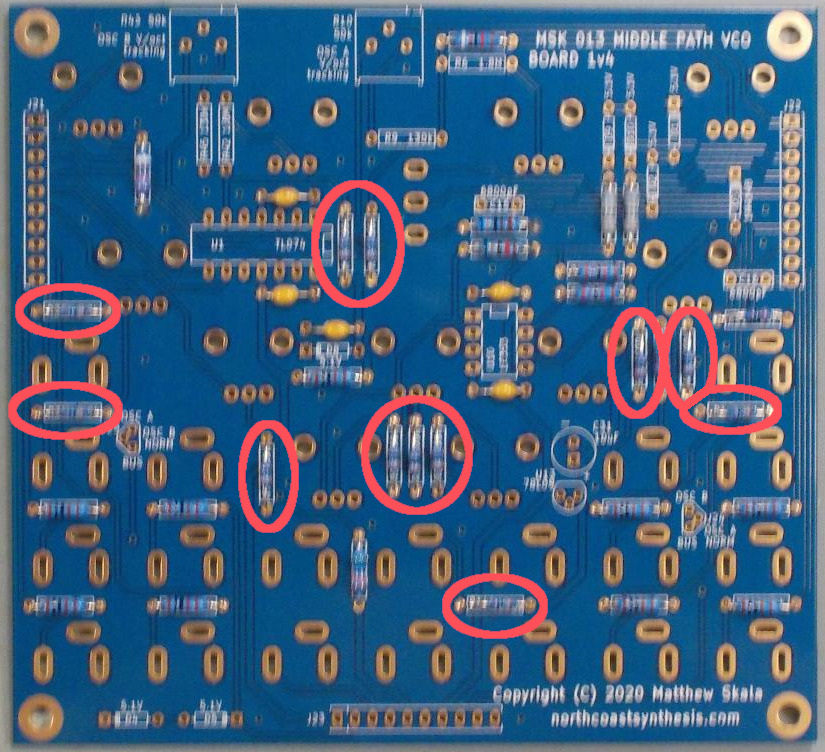
\includegraphics[width=\linewidth]{res-100k1.jpg}

\pagebreak

Install the 150k$\Omega$ (brown-green-black-orange) resistor R55.
This resistor sets the DC normalization for the VCA control input.

\nopagebreak
\noindent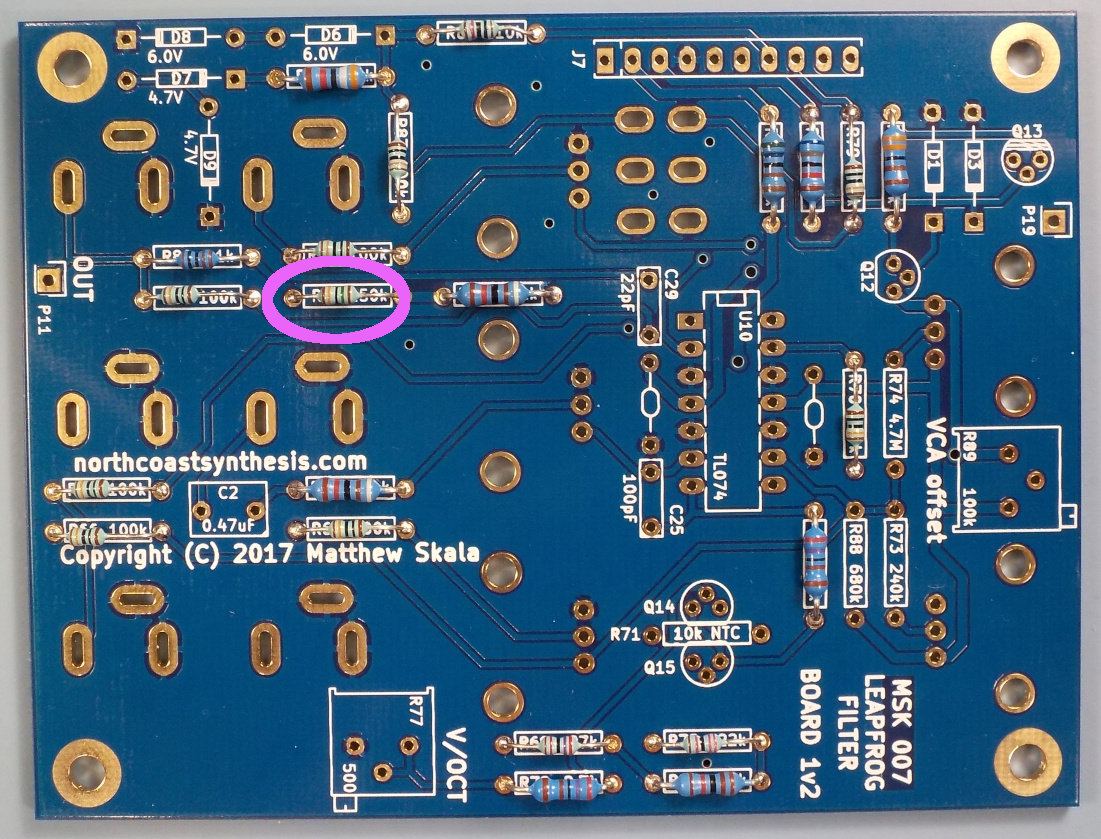
\includegraphics[width=\linewidth]{res-150k1.jpg}

Install the 240k$\Omega$ (red-yellow-black-orange) resistor R73.
This resistor sets the range of the coarse tuning knob to about ten
octaves.

\nopagebreak
\noindent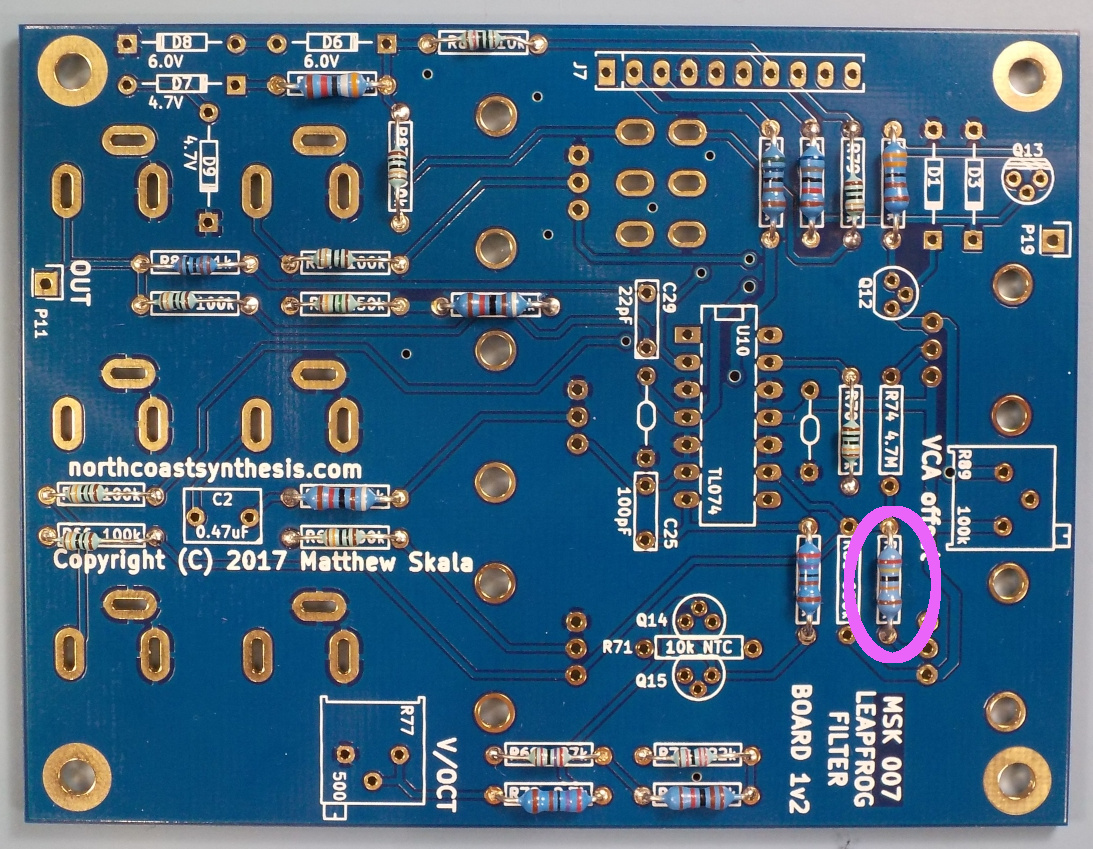
\includegraphics[width=\linewidth]{res-240k1.jpg}

\pagebreak

Install the 680k$\Omega$ (blue-grey-black-orange) resistor R88.
This resistor sets the overall offset of the tuning knobs, for a
non-guaranteed design target of approximately 10Hz to 10kHz cutoff frequency
with zero pitch control voltage.

\nopagebreak
\noindent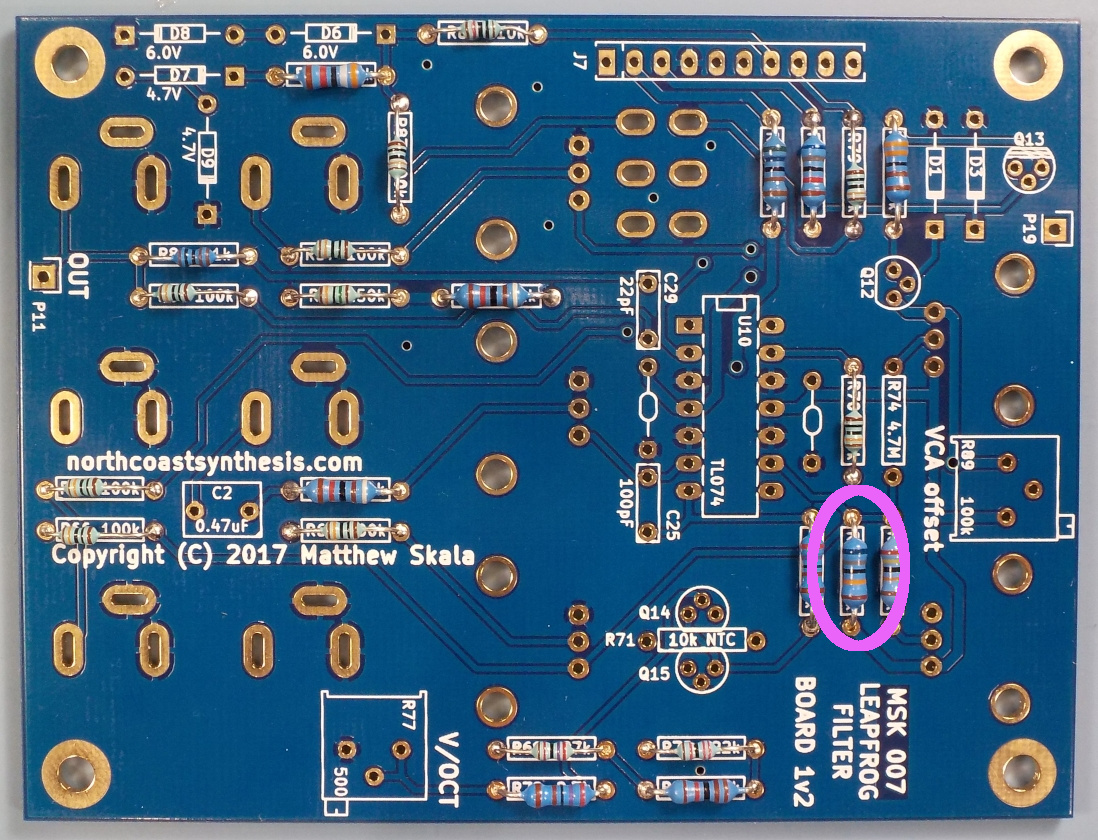
\includegraphics[width=\linewidth]{res-680k1.jpg}

Install the 4.7M$\Omega$ (yellow-violet-black-yellow) resistor R74.
This resistor sets the range of the fine tuning knob to about half an
octave.

\nopagebreak
\noindent\includegraphics[width=\linewidth]{{res-4.7m1}.jpg}

\section{Diodes}

There are six diodes to be mounted on Board~1:  two each of 1N4148 or 1N914
switching diodes; 1N5230B 4.7V Zener diodes; and 1N5223B 6.0V Zener diodes. 
They all look like pretty much identical orange-pink glass beads, and it is
important not to confuse them.  Their bodies will be marked with type
numbers in very small print, and they should be labelled in a kit, but if
you are in any doubt, test them for breakdown voltage.

\pagebreak

To do a breakdown voltage test:  use clip leads or a breadboard to connect
the diode under test in series with a small resistor (anything from
1k$\Omega$ to 10k$\Omega$) reverse biased across a 12V power supply.  That
is, the power supply positive connects to one end of the resistor, the other
end of the resistor connects to the cathode (striped end) of the diode, and
the anode (other end) of the diode connects to the power supply negative. 
Then measure the voltage across the diode.  It should be close to the
specified Zener voltage of 4.7V or 6.0V if you are testing a Zener diode,
and equal to the power supply voltage if you are testing one of the
switching diodes.  From that it should be possible to determine which diodes
are which.  If the measured value is less than 1V, then you most likely have
the diode backwards and are measuring its \emph{forward} voltage, which will
be about the same for all three of these diode types and is not a useful way
to distinguish them.

All these diodes are polarized components and it is important to install
them right way round.  Each diode has a black stripe at one end; that end is
the \emph{cathode}.  The silkscreen markings on the board have a
corresponding stripe and the diodes should be installed with their stripes
matching the markings on the board.  The solder pads for the cathodes are
also square instead of round.

Install the two 1N4148 or 1N914 switching diodes D1 and D3.  These are used
to control the minimum base voltages for the transistors in the VCA section.

\nopagebreak
\noindent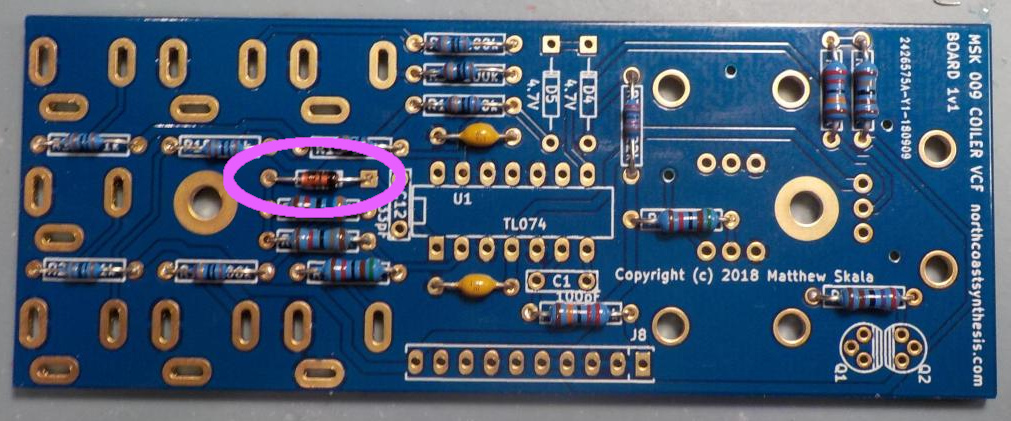
\includegraphics[width=\linewidth]{1n4148.jpg}

\pagebreak

Install the two 1N5230B Zener diodes D7 and D9.  Their breakdown voltage of
4.7V is marked on the silkscreen as an additional guide to where they go. 
These set the lower voltage level for the soft-clipping circuit.

\nopagebreak
\noindent\includegraphics[width=\linewidth]{{zener-4.7v1}.jpg}

Install the two 1N5233B Zener diodes D6 and D8.  Their breakdown voltage of
6.0V is marked on the silkscreen as an additional guide to where they go. 
These set the higher voltage level for the soft-clipping circuit.

\nopagebreak
\noindent\includegraphics[width=\linewidth]{{zener-6.0v1}.jpg}

\section{DIP sockets}

Install the 14-pin DIP socket for the TL074 quad op amp chip U10.  The
amplifiers in this chip are used in the exponential converter and as buffers
between the filter core and the outside world.  See
page~\pageref{pag:dip-sockets} for notes regarding orientation of the
socket, procedure for soldering it flat to the board, and so on.

\noindent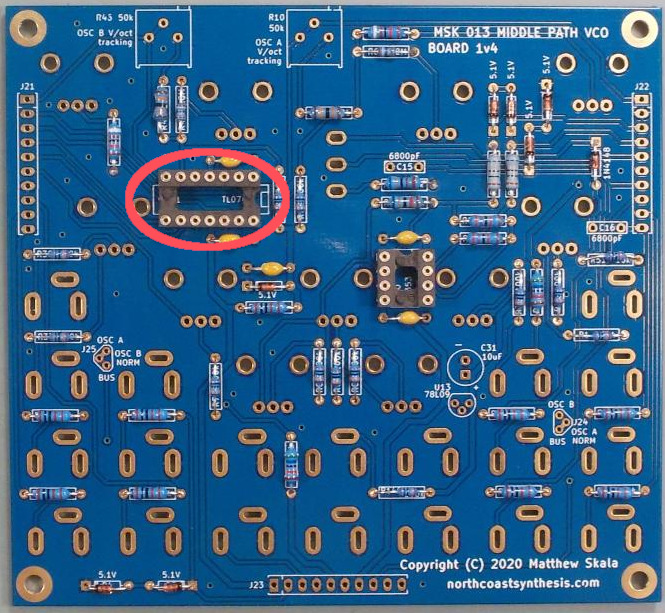
\includegraphics[width=\linewidth]{dip14-1.jpg}

\section{Trimmer potentiometers}

If you have not already set the trimmers to 50\%\ of their full scale value
as described under ``Preliminaries'' above, then do it now.

Trimmers are not exactly polarized, but the three legs of each trimmer serve
different functions and need to be connected to the right holes.  The
physical arrangement of the legs and corresponding holes should make it
impossible to install the trimmers wrong way round.

Install the 500$\Omega$ trimmer R77.  This trimmer sets the scale factor for
the V/octave pitch CV, an adjustment often called ``tracking.''

\nopagebreak
\noindent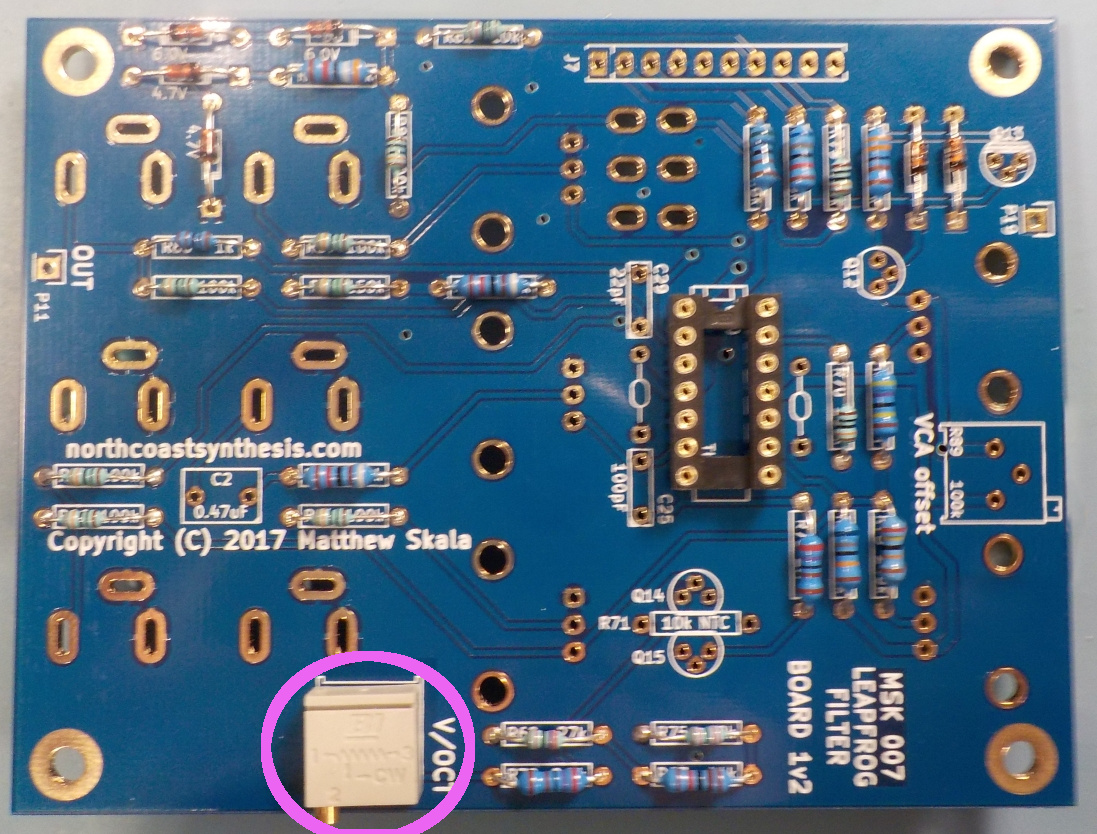
\includegraphics[width=\linewidth]{pot-500w1.jpg}

\pagebreak

Install the 100k$\Omega$ trimmer R89.  This trimmer adjusts the DC offset in
the VCA section.

\nopagebreak
\noindent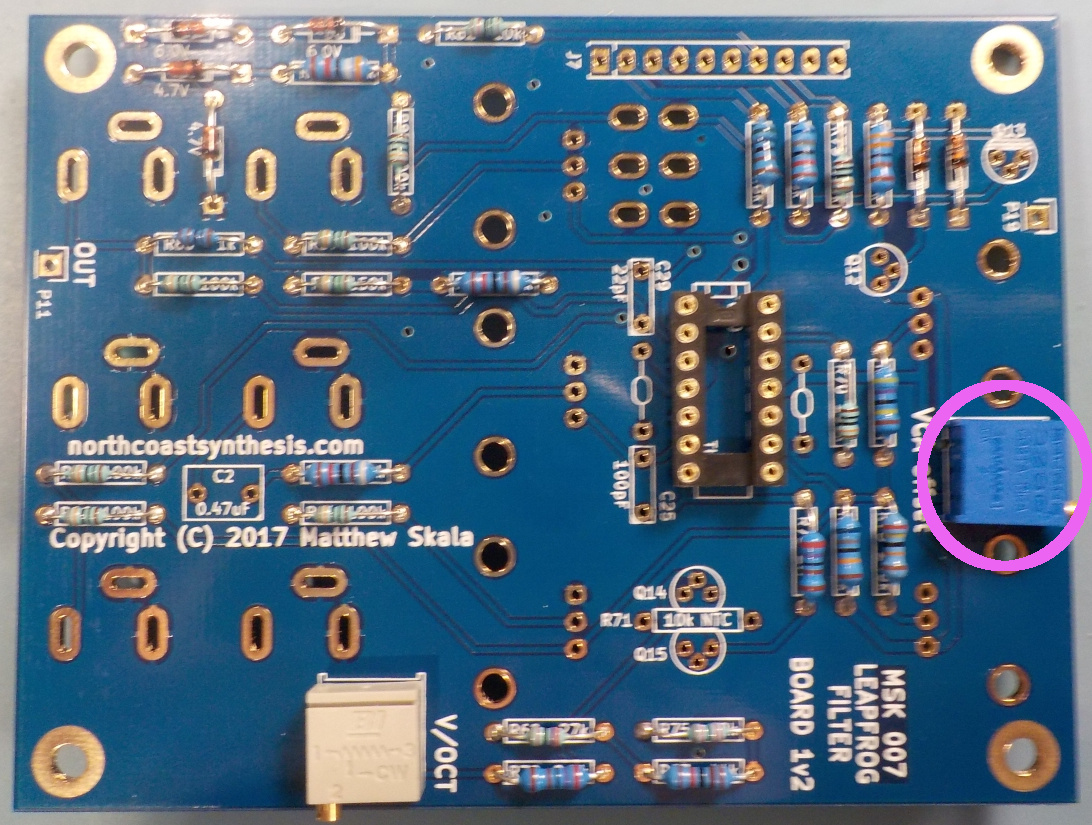
\includegraphics[width=\linewidth]{pot-100k1.jpg}

\section{Capacitors}

Small-valued ceramic capacitors are usually labelled with numbers in a
pattern similar to the resistor colour code:  two digits for the main value,
followed by a third digit that says how many zeroes to append to get the
value in picofarads.  Thus the 22pF capacitor may be labelled ``220'' and
the 100pF capacitor ``101.''  Other markings on the capacitor body may
indicate tolerance, voltage rating, dielectric type, and so on.  The
0.1$\mu$F decoupling capacitors will probably have very abbreviated markings,
but if they are labelled on the three-digit system the code would be ``104''
for 0.1$\mu$F $=$ 100000pF (10 followed by 4 additional zeroes);
and the box-type 0.47$\mu$F film capacitor will likely be marked with its
value in microfarads using $\mu$ instead of the decimal point, thus
``$\mu$47.''  None of the capacitors to be installed on this board are
polarized.

\pagebreak

Install the 22pF ceramic capacitor C29.  This capacitor prevents
high-frequency oscillation of the output driver op amp.

\nopagebreak
\noindent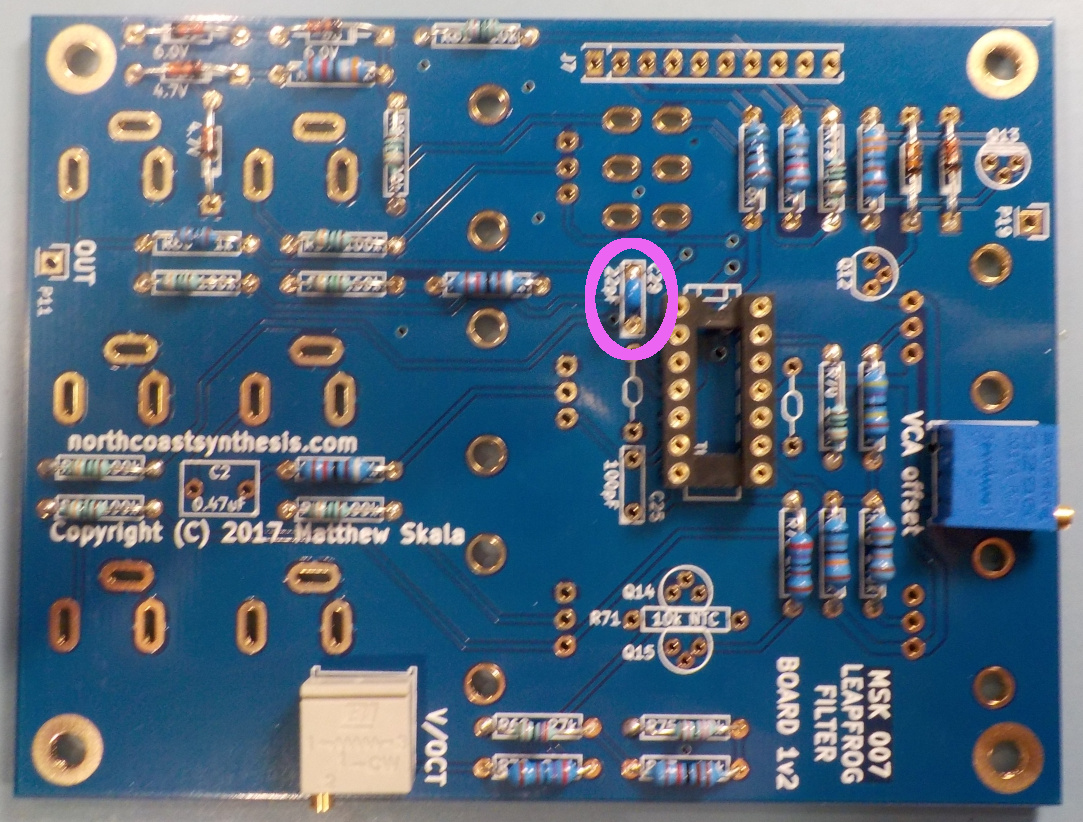
\includegraphics[width=\linewidth]{cap-22p1.jpg}

Install the 100pF ceramic capacitor C25.  This capacitor prevents
high-frequency oscillation of the exponential converter servo op amp.

\nopagebreak
\noindent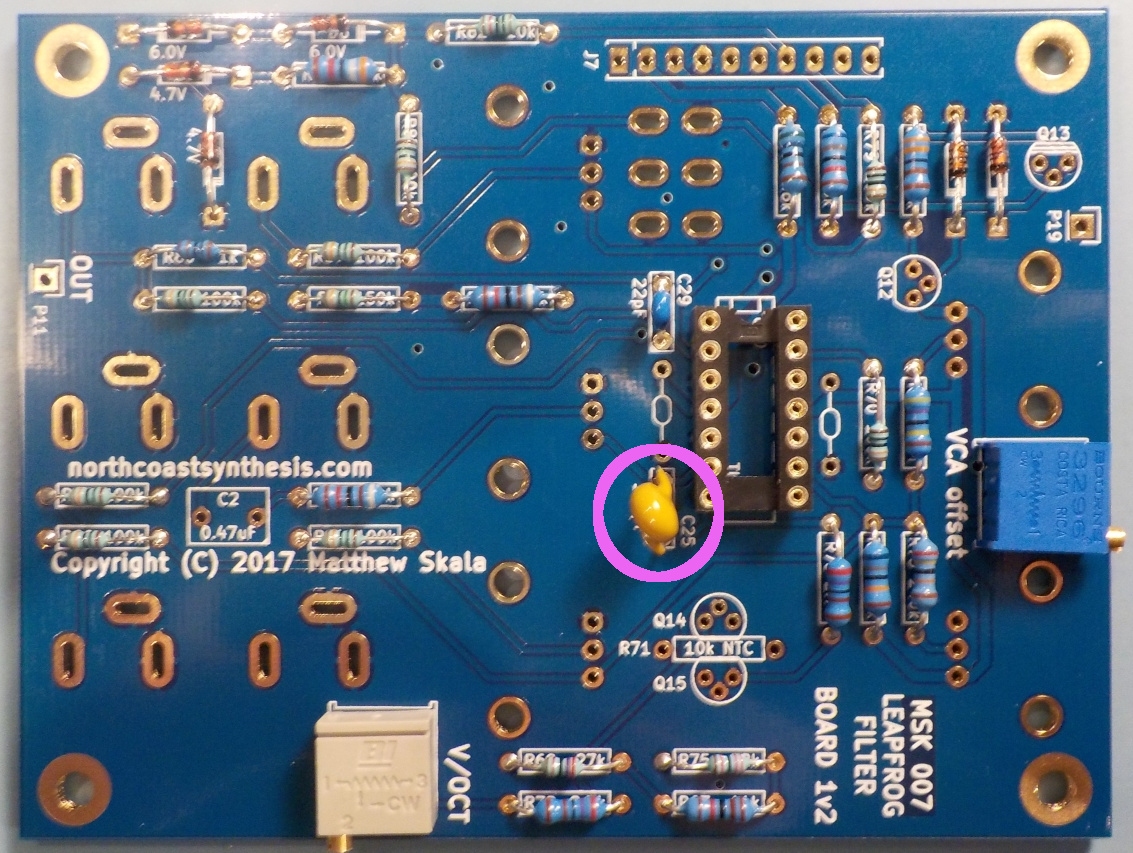
\includegraphics[width=\linewidth]{cap-100p1.jpg}

\pagebreak

Install the two 0.1$\mu$F decoupling capacitors.  As described on
page~\pageref{pag:decoup-symbol}, they are shown on the board silkscreen by
a special symbol without values or reference designators.  They filter the
power supplies for the op amp chip.

\nopagebreak
\noindent\includegraphics[width=\linewidth]{{cap-0.1u1}.jpg}

Install the 0.47$\mu$F film capacitor C2.  This capacitor provides AC
coupling for the linear FM input.

\nopagebreak
\noindent\includegraphics[width=\linewidth]{{cap-0.47u1}.jpg}

\pagebreak

\section{TO-92 semiconductors}

See page~\pageref{pag:to-92} for general instructions regarding TO-92
semiconductors and the board symbols used for them.

Install the PNP transistor Q13, type SS8550D or PN200A.  This transistor
acts as a current source for controlling the VCA section.

\nopagebreak
\noindent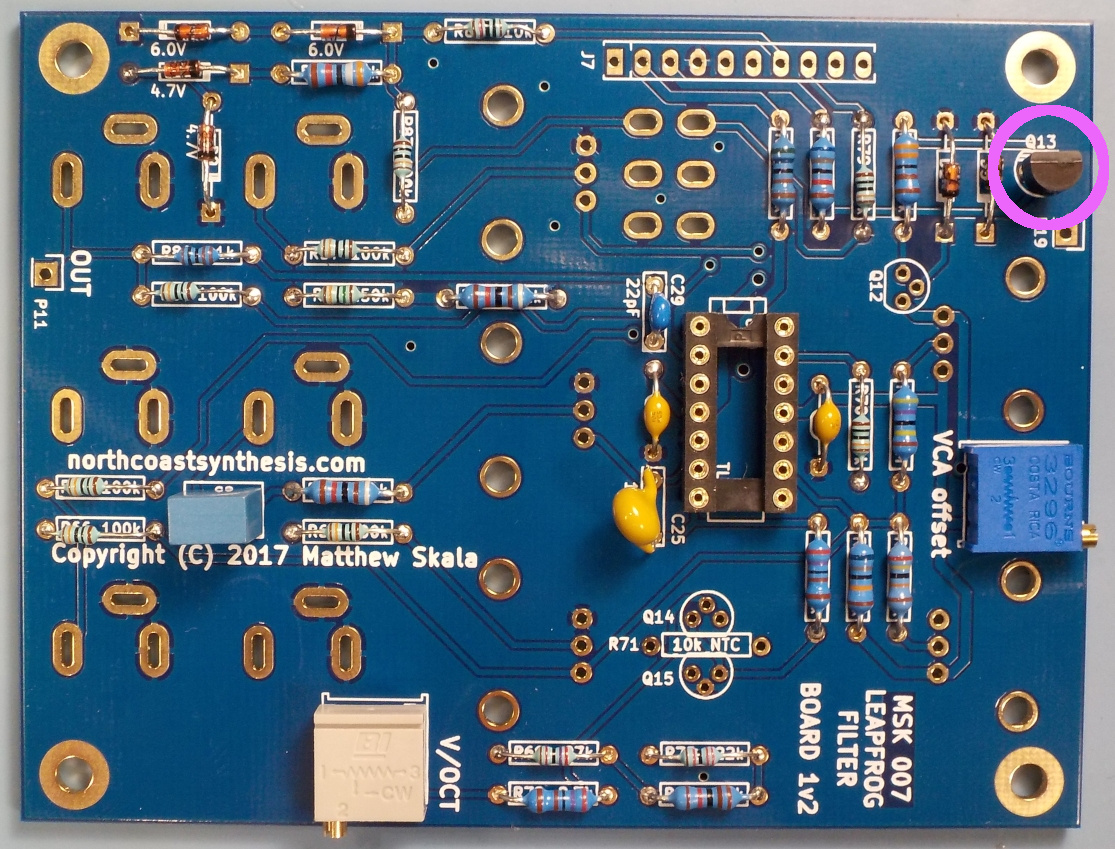
\includegraphics[width=\linewidth]{pn200a-1.jpg}

Install the 2N5088 NPN amplifier transistor Q12.  This transistor acts as an
emitter follower to translate the input control voltage to a current for
Q13.  There are two more 2N5088 transistors to be installed in the next
section.

\nopagebreak
\noindent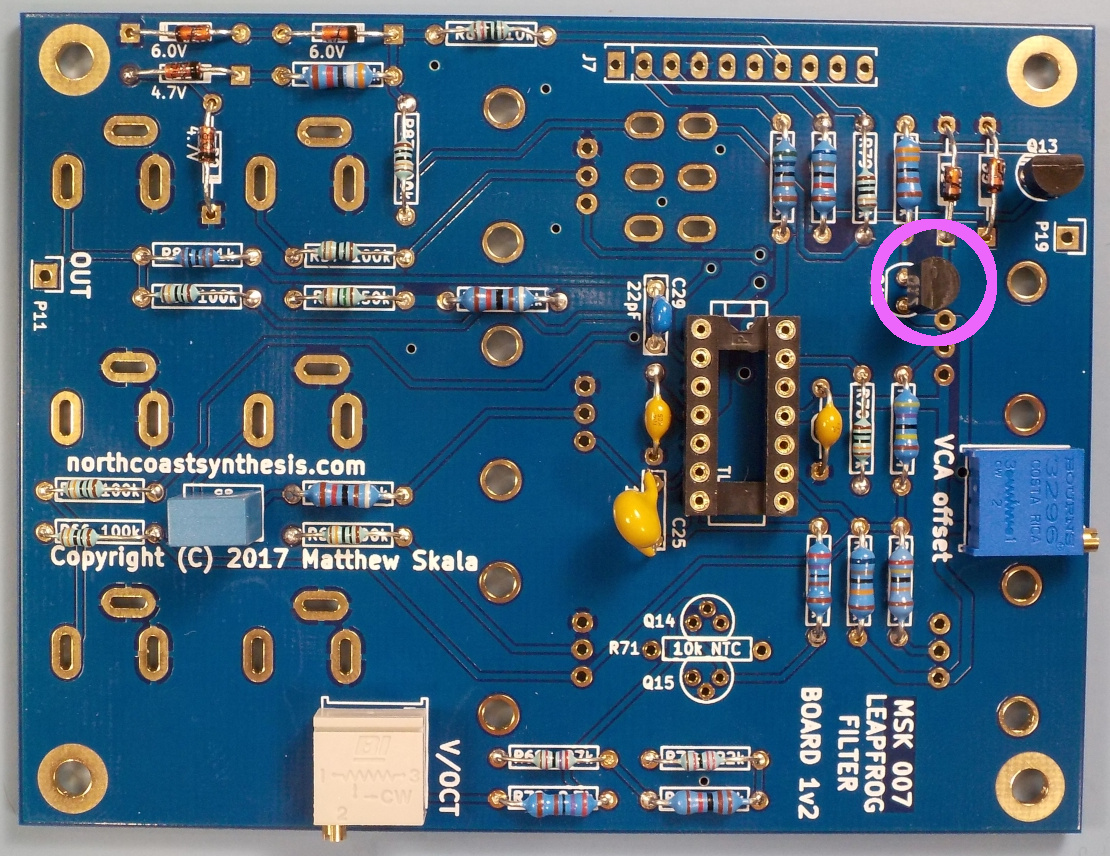
\includegraphics[width=\linewidth]{2n5088-1.jpg}

\section{Exponential converter cluster}

In order to reduce the temperature dependence of the exponential converter
as far as possible, is is important that the two transistors Q14 and Q15,
and the thermistor (temperature-sensitive resistor) R71, should all be kept
at the same temperature.  This is accomplished by mounting them all in
contact with each other and tightening a nylon cable tie around them to keep
them pressed together.  Constructing this cluster of components is a little
tricky and annoying; follow the directions carefully.

Bend the thermistor legs as shown:  one leg straight down, the other down
about 3mm, then to the side, then down again, to fit the R71 footprint. 
Place the thermistor in its footprint, but do not solder it yet.

\nopagebreak
\noindent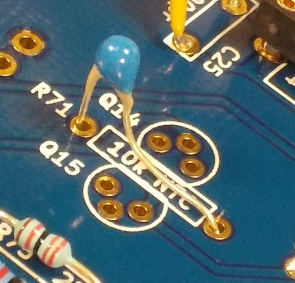
\includegraphics[width=\linewidth]{ntc-bend.jpg}

Insert the two 2N5088 transistors Q14 and Q15 in the board, face to face as
shown.  Do not solder them yet.

\nopagebreak
\noindent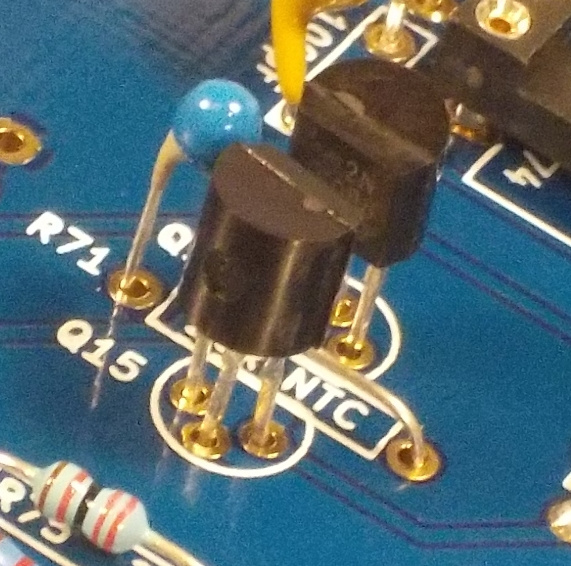
\includegraphics[width=\linewidth]{expo-untied.jpg}

\pagebreak

Put a nylon cable tie around the three components and tighten it far enough
to hold them loosely together.  Concentrate in particular on having the two
transistors meet as cleanly face to face as possible.  Do not overtighten
the cable tie or cut it off yet.  This is probably the hardest step, and
North Coast kits include a spare cable tie for use in case you ruin one.  Be
aware that the components should not stick out any further above the board
than is normal for other TO-92 components; if you seat the transistors too
high up, at the full length of their legs, you may exceed the 11mm of
clearance between this board and Board~2 above it.

Solder the components.  Then tighten the cable tie the rest of the way and
cut off the excess.

\nopagebreak
\noindent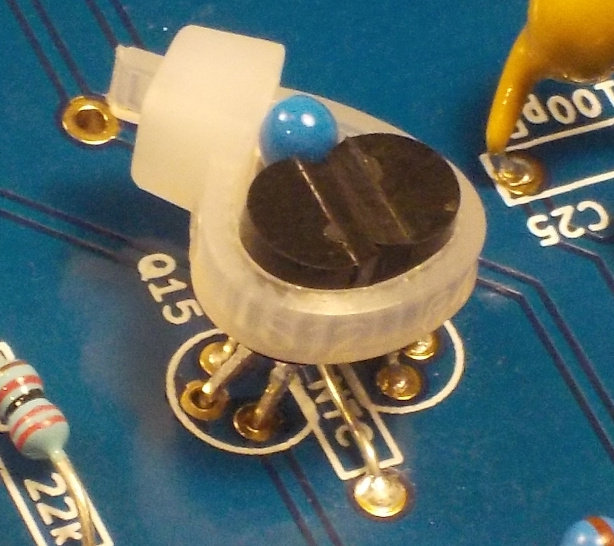
\includegraphics[width=\linewidth]{expo-tied.jpg}

\pagebreak

\section{Board to board connectors}

Screw one 13mm and one 11mm standoff into each of the four mounting holes in
Board~1, as shown.  The shorter (11mm) standoff should be on the top, the
same side as the components already installed, with the male-threaded ends
sticking up.  These standoffs will separate Board~1 from Board~2 in the
final module.  The longer (13mm) standoffs should be on the bottom, with
their male ends passing through the board to mate with the 11mm standoffs.

\nopagebreak
\noindent\includegraphics[width=\linewidth]{board12-stack-1.jpg}

Mate the 10$\times$1 header connectors J7 and P26 and place them (do not
solder yet) in the J7 footprint on Board~1 with the legs of the female
connector J7 going through the board.

\nopagebreak
\noindent\includegraphics[width=\linewidth]{board12-stack-2.jpg}

\pagebreak

Place your completed Board~2 from the previous chapter on top of the
assembly, component side up with the legs of P26 going through the P26
footprint, and fasten it with the remaining four 11mm standoffs.

\nopagebreak
\noindent\includegraphics[width=\linewidth]{board12-stack-3.jpg}

Solder J7 and P26 in place on the two boards.  Then remove Board~2 and the
four standoffs holding it in place, but keep the standoffs that go through
the holes in Board~1.

\section{Panel components}

Flip Board~1 over; you will now be installing the components that go between
it and the panel.  The exact details of how the pieces fit together are
important and may not be obvious; see the exploded assembly diagram on
page~\pageref{fig:exploded}, which may clarify things.

The toggle switch SW3 is for switching the VCA section between providing
feedback and controlling the output.  It has a body just a little shorter
than will fit well into the 13mm space between Board~1 and the panel.  This
space is forced to be 13mm to accommodate the potentiometer bodies.  The
switch comes with two nuts and only needs one for fastening on the front of
the panel.  We use the second one as a spacer behind the panel to hold the
switch body far enough back that its legs will go through the holes in the
board.  Remove and save the hardware from the switch bushing, then screw on
one of the nuts all the way down to the bottom of the bushing.

The switch's electrical connections are symmetrical, but it has a slot or
keyway in its bushing, used to hold the special anti-rotation washer in
place.  This keyway must face toward the outer edge of the board in order
for the anti-rotation washer to be able to connect \pagebreak the switch
properly with a matching small hole in the panel.  Place (do not solder yet)
the switch in its footprint on Board~1, with the keyway facing outward.

\nopagebreak
\noindent\includegraphics[width=\linewidth]{switch-keyway.jpg}

Place (do not solder yet) the five panel control potentiometers R56, R62,
R69, R78, and R81 in their footprints on the board.  These provide manual
control of the module's functions.  Place (do not solder
yet) the six phone jack sockets J1 through J6 in their footprints.  These
are for patching signals to and from other modules.  All these components
should only be able to fit into the board in one way.

\nopagebreak
\noindent\includegraphics[width=\linewidth]{panel-components.jpg}

Line up the panel on top of the asembly and fasten it in place by driving
the four machine screws through their corresponding holes into the 13mm
standoffs.  Double check that the keyway on the switch bushing is facing the
small hole near the switch which will accept the alignment tab from the
anti-rotation washer.

\noindent\includegraphics[width=\linewidth]{panel-screws.jpg}

Install all the hardware for the panel components.  In the case of the
switch, the sequence is first (nearest the panel) the anti-rotation washer,
with one of its tabs fitting into the keyway on the bushing and the other
sticking into the small panel hole provided for this purpose; then the
toothed lock-washer (sharper side of the teeth facing up to engage with the
nut, if there's a noticeable difference between the two sides); and finally
the nut.  In the case of the potentiometers, the sequence is first (nearest
the panel) the conical spring washer, high side in the middle and low side
around the outside; then the toothed lock-washer; then the nut.

In the case of the jack sockets, the knurled nuts provided for these will
have screwdriver slots on one side, and those should face the outside with
the smoother side facing the panel.  You may need to tilt the assembly and
jiggle it a bit to get the jack sockets to fall into the right alignment
with their bushings poking through the panel.  On the other side, when
correctly installed their solder legs (and those of the switch) will just
barely pass through the circuit board.

Do not overtighten any of this hardware, and be careful, if you are
using wrenches or pliers, to avoid scratching the panel.  Wrapping the tool
jaws with tape may help.

\nopagebreak
\noindent\includegraphics[width=\linewidth]{panel-hardware.jpg}

Solder the panel components.  It can be tricky to do the joints where a
component leg just barely passes through the board, but if you take it slow
and make sure that the PCB hole is filled with solder and the whole joint is
liquid before you remove the heat, then you can be reasonably sure that you
have wetted the leg and made a good electrical connection.  It may help to
use a larger-than-usual soldering iron tip if you have one.

\pagebreak

\section{Final assembly}

Attach the knobs to the potentiometers.  Twist each shaft to its limits in
each direction to ascertain how the slot in the shaft corresponds to where
you want the knob pointer, then slide the knob onto the shaft in the correct
orientation and tighten the setscrew with a small flat screwdriver.  See the
comments at the start of this chapter about knobs, and be sure not to
overtighten the setscrews when attaching them.

Insert a TL047 chip in the U10 socket on Board~1.  Be careful to insert it
right way round: the end with Pin 1 will be marked by an indentation at one
corner or a notch in the end and this end of the chip should be inserted to
match the notch in the socket and on the board silkscreen and the
rectangular Pin 1 solder pad.

Also be careful that all the legs of the chip go into the corresponding
holes in the socket.  These chips, when brand new, usually have their legs
splayed outward a little bit (a measure intended to help them fit snugly
into circuit boards when used without a socket) and you must gently bend the
legs inward in order to fit them in the sockets.  If you apply pressure to a
chip prematurely, without all the legs properly fitting into the holes, it
is easy to have the legs fold up or even break off.

It should not be necessary to remove the panel from Board~1 again.  Attach
Board~2, carefully fitting its header plug into the header socket on Board~1
and the male ends of the standoffs through the corresponding holes in Board~2. 
Screw on the remaining 11mm standoffs to hold it in place.

Insert the remaining four TL074 chips and the three LM13700 chips in their
corresponding sockets.  See the notes above on inserting DIP chips in
general, and pay special attention to the directional markings on the board
silkscreen and the notches in the sockets to make sure you have them
installed in the right directions.

If you have not yet done the ``pre-adjustment'' described in the next
chapter, do it now, before assembling Board~3 with the rest of the module. 
But assuming that is complete, add Board~3 to the assembly, fitting its
three male header connectors into the header sockets on Board~2, and screw
on the four hex nuts to hold it in place.  Be careful with your nutdriver,
pliers, or other tools not to damage other components near the nuts on
Board~3.  If using a nutdriver, socket wrench, or similar, be careful not to
overtighten the nuts:  some tools make it easy to apply more torque than the
threads can sustain.

\pagebreak

There is a rectangular white area on Board~3
reserved for adding a serial number, signature, quality control marking, or
similar.  Use a fine-tipped permanent marker to write whatever you want
there.

Your module is complete.

\nopagebreak
\noindent\includegraphics[width=\linewidth]{finished-module.jpg}

% $Id: calibration.tex 9912 2022-03-20 19:17:14Z mskala $

%
% Firmware update and calibration
% Copyright (C) 2022  Matthew Skala
%
% This program is free software: you can redistribute it and/or modify
% it under the terms of the GNU General Public License as published by
% the Free Software Foundation, version 3.
%
% This program is distributed in the hope that it will be useful,
% but WITHOUT ANY WARRANTY; without even the implied warranty of
% MERCHANTABILITY or FITNESS FOR A PARTICULAR PURPOSE.  See the
% GNU General Public License for more details.
%
% You should have received a copy of the GNU General Public License
% along with this program.  If not, see <http://www.gnu.org/licenses/>.
%
% Matthew Skala
% https://northcoastsynthesis.com/
% mskala@northcoastsynthesis.com
%

\chapter{Firmware update and calibration}

Many of the Gracious Host's features are defined by \emph{firmware} -- that
is software built into the hardware -- and it is possible to replace the
firmware on an existing module with a new version.  Before attempting a
firmware update you should make sure you know \emph{why} you are updating
your firmware.  If your module works and you are satisfied with it, you may
not need to make any changes.  The update process involves some risk and
should not be attempted for no reason.  But it is possible that I, or third
parties, may release enhanced firmware with special features in the future. 
You may also have created new firmware of your own using the information in
the \emph{MSK~014 Gracious Host Programmer's Manual}.

After loading the firmware, the module also needs \emph{calibration}, which
adjusts the mapping between analog values in the outside world and digital
values used in the firmware, to account for component values and
module-to-module variation.  The calibration process is mostly automated.  It
involves using a standard V/oct VCO as a reference.

If you have built your own module, it will need to be calibrated.  Running
the firmware update is one way to accomplish that, but you can also plug in
a typing keyboard and enter maintenance code 5833, as described in the
chapter on typing keyboards, to run the calibration procedure without
updating firmware first.

To complete the update and calibration process, you will need:
\begin{itemize}
  \item The Gracious Host module;
  \item a V/octave VCO that can track reasonably well over 0V--5V control
    voltage input;
  \item a couple of patch cables and the necessary power supply to run both
    modules at once;
  \item a USB flash drive and computer capable of writing files to it; and
  \item the firmware image file you want to use.
\end{itemize}

\section{Preparing a firmware image}

You will need an \emph{image file}, which contains the executable firmware
code in a special format specific to the Gracious Host.  Up-to-date official
firmware images are available from the North Coast Synthesis Web site at
\url{https://northcoastsynthesis.com/}, as is the source code.  Third-party
firmware images may be available elsewhere.

The official firmware is subject to the GNU General Public License, and so
must be any others that include parts of it.  Among other things, that means
third-party distributors of installable binary images are required to
share their source code if their images contain any part of the original
firmware.

The process of loading new firmware depends on code included in the
\emph{old} firmware.  It is possible that loading a bad firmware image may
``brick'' your module, making it unable to load any further updates through
USB.  For that reason, you should be careful about loading unknown or
untested firmware images.  The module will not load an image file that fails
a check of the CRC32 values included in the file, so mere file corruption is
unlikely to result in a bricked module.  But buggy code correctly packaged
could possibly be a problem.

Prepare a USB flash drive in the format typically used by Windows.
Most other popular operating systems can also format flash drives
this way.  The default settings should work.  In more detail: the drive
needs to have at most $2^{32}$ blocks, which translates to a maximum
capacity of 2T if the blocks are standard 512-byte size; FAT12, FAT16, and
FAT32 should all work, with FAT32 having received the most thorough testing;
and the filesystem needs to be either written to the entire drive, or in a
primary (not extended) partition described by a standard DOS partition
table.

Rename the firmware to ``FIRMWARE.FRM'' if that is not already its name, and
put the file in the root directory of the flash drive.  The module will
ignore all subdirectories and all files with other names.

\section{Firmware update}

Power up the module, and insert the flash drive.  The module will
automatically detect the drive, scan it for a valid firmware file, and
attempt to reflash itself with the new image.  That normally takes less than
a second.  If the update succeeds, the module will start the calibration
process, below, with slow-flashing red LEDs.

If firmware update fails, the module will perform the \emph{failure
display}, which consists of both LEDs flashing red slowly (1\,Hz, 50\%\ duty
cycle) and an ominous tune played in 0V--9V square waves on the digital output
jacks.  If you patch either output jack to a speaker or headphone (beware of
the DC offset; putting it through an AC-coupled module of some kind might
help) you can hear this.

\qquad\includegraphics{failure.cropped.eps}

\blinkcodeLR{}{4/8}{}{4/8}

The failure display lasts one minute, after which (if you haven't powered it
off already) the module will reboot.  If you leave the flash drive inserted
throughout this, then it will attempt the update again as soon as it does
reboot.

If the module is unable to even attempt the firmware update -- for instance,
because it cannot interface with the flash drive -- then instead of the
slow-flash failure display it may flash the LEDs back and forth very fast, in
red, until the flash drive is removed.

\blinkcodeLR{}{0/0.5,1/1.5,2/2.5,3/3.5,4/4.5,5/5.5,6/6.5,7/7.5}%
{}{0.5/1,1.5/2,2.5/3,3.5/4,4.5/5,5.5/6,6.5/7,7.5/8}

There is not a lot that can be done to debug a failed update.  Possible
causes might include:
\begin{itemize}
  \item a badly-prepared firmware file, or one actually intended for some
    other module;
  \item something wrong with the transfer of the file -- for instance, if
    you do not actually have the entire file;
  \item something wrong with the flash drive formatting or preparation, so
    that the module cannot \emph{find} the file;
  \item an unusual, incompatible flash drive; or
  \item hardware problems (perhaps more likely in a DIY situation),
    especially affecting the microcontroller's communication with the
    SRAM chip.
\end{itemize}

In most plausible failure cases the module should retain its old firmware
unchanged after a failed update attempt, though I cannot promise that in
every case.  Attempting the update again after a failure should be safe, but
it will probably just fail again if nothing has changed.

\section{Calibration:  general remarks}

The firmware needs to know what numbers to send to the DACs to produce
specific output voltages, and what numbers it can expect from the ADCs when
it receives specific input voltages.  These are called output calibration
and input calibration respectively.  Although the firmware comes with
reasonable guesses built in, the exactly correct numbers will be different
on each individual module because of natural variations in the components
used to build them.

The Gracious Host does not contain any very accurate voltage reference that
could be used for calibration, but it \emph{does} have an accurate clock
crystal, so it can measure times and frequencies to a precision that is more
than good enough for rock'n'roll.  The calibration process takes advantage
of that ability by using an external VCO to convert voltages into
frequencies.  Most users will have a VCO, because one of the main purposes
of the Gracious Host is to control a VCO anyway.  The Gracious Host output
calibration sends different numbers to the DACs, accurately measures the
resulting VCO frequencies, and infers the voltages it must be producing. 
Then once the output voltages are known, they can be used to calibrate the
input voltages.

One consequence of doing things this way is that your Gracious Host's
voltage calibration is only as good as that of the VCO used to do it.  If
the VCO's tracking is off, the Gracious Host's voltages will be off in the
same way.  However, if you intend to usually use the Gracious Host with
\emph{that same VCO}, at a single standard tuning setting, then matching the
VCO's errors can be a virtue.  The Gracious Host's output voltages will end
up calibrated to whatever voltages that particular VCO needs to give in-tune
pitches, compensating for the tracking error, because the calibration was to
the VCO's frequencies rather than the voltages that a perfect VCO would
require.  The inaccuracy would only become an issue if you subsequently
tried to use the Gracious Host with some other VCO, or with the VCO's tuning
significantly different from where it was when you did the calibration.

The calibration routine is multi-threaded and the left and right sides work
independently, so you can concentrate on just one side and do it completely
before working on the other; you can do output on one side, then the other,
and then do input; or if you have two suitable VCOs you can do both sides at
once.

\section{Output calibration}

Calibration of either channel starts with the LED on that channel's side
blinking red, in long slow pulses with short gaps between them (1.05\,s
overall cycle time).

\blinkcodeX{}{0/7}

When you see these blinks, any firmware update as such has already
completed.  It is safe to remove the USB drive at this point, and you should
remove it before the end of the calibration process.

Tune your VCO so that at 0V input it will produce a frequency between 31\,Hz
and 277\,Hz.  If your VCO tracks well then the exact frequency does not
matter much here, because the Gracious Host is only measuring the VCO's
response to voltage, which ought to be the same across a wide frequency
range.  If your VCO does not track well and you are relying on the Gracious
Host to correct the VCO's tracking errors, then you should tune it the way
you normally will.  For standard MIDI concert pitch that would ideally be
65.406\,Hz at 0V (that is the C two octaves below Middle~C), but the
measurement range allows for tuning the VCO down an octave or up as much as
two octaves relative to standard MIDI.

Turn off any sync, modulation, waveshaping, and similar features of the VCO. 

Patch the analog (CV) output from the Gracious Host channel you are
calibrating, into the VCO's V/octave control voltage input.  Do this before
patching the VCO output.

Patch the VCO output into the input of the Gracious Host channel you are
calibrating.  Use the square wave output if the VCO has one; if not, use any
simple waveform, such as sine, sawtooth, or triangle.  The Gracious Host
uses an input threshold of approximately $+$1.62V, and you want a waveform
that will pass through that voltage once in the upward direction and once in
the downward direction on each cycle.

This image shows both channels of a Gracious Host hooked up for output
calibration using the two cores of an MSK~013 Middle Path VCO; but remember
that it is not necessary to have a dual VCO.  You could use a single VCO for
both sides, doing them one at a time.

\nopagebreak\noindent
{\hspace*{\fill}\includegraphics[scale=0.45]{calpatch1.png}\hspace*{\fill}\par} 

The module will automatically detect when a suitable VCO signal is present,
and will start sending different control voltages and measuring the
resulting frequencies.  It is trying to adjust the voltages for ten
different notes, while also re-confirming the frequency at 0V.  As more of
the voltages are detected as on-target, the red flashes get shorter while
keeping the same repetition rate of one flash every 1.05\,s.  When nearly
complete the LED will be off most of the time with only brief red flashes.

\blinkcodeX{}{0/2}

You can follow the progress of the output calibration by watching the length
of the flashes.  How long it takes depends on the VCO's stability and how
far the previous calibration was from the new one, but it is normally
expected to complete in less than a minute, and it may be only two or three
seconds if the previous calibration almost perfectly matches the new one.

When output calibration completes the channel will wait to be repatched for
input calibration.

\section{Input calibration}

When the channel is ready for input calibration it switches to a
faster blink pattern in alternating green and red.

\blinkcodeX{0/3.5}{4/7.5}

For this step, disconnect the VCO and just patch the Gracious Host's analog
output directly to its own analog input on the same side.  This diagram,
like the last one, shows both channels so patched, but remember that the
channels are independent and you can do input calibration on one of them
while the other is at a different stage.

\nopagebreak\noindent
{\hspace*{\fill}\includegraphics[scale=0.45]{calpatch2.png}\hspace*{\fill}\par} 

In principle, the input calibration will shorten its LED blinks to indicate
progress, in the same way that the output calibration did.  However, the
input calibration is usually so fast (two or three seconds per channel) that
you may not see the shorter blinks before it finishes.

\blinkcodeX{0/0.5}{4/4.5}

When one channel has completed input calibration, it will display quite fast
green blinks (3.8\,Hz, 50\% duty cycle) while it waits for the other.

\blinkcodeX{0/1,2/3,4/5,6/7}{}

When \emph{both} channels complete input calibration, both LEDs will go
solid green as part of the \emph{success display}, and the digital output
jacks will play a happy tune in 0V--9V square waves.  You can patch either
output jack to a speaker or headphone (remaining aware of the 4.5V DC
offset) to hear this.

\includegraphics{success.cropped.eps}

\blinkcodeLR{0/8}{}{0/8}{}

The success display lasts one minute, after which the module will reboot. 

If you initiated calibration by doing a firmware update, then you ought to
have already disconnected the USB drive before the end of the success
display; otherwise, on reboot it will attempt to update the firmware again. 

The calibration data is written to the module's non-volatile memory at the
\emph{start} of the success display, so it is safe to power down the module
as soon as you see the solid green LEDs.  If you wish to abort calibration
once started, just power the module down before reaching the end.  In that
case, the module will end up with the default values from the firmware you
loaded, if you loaded firmware; or no change to the existing calibration if
you started calibration in some other way, such as with maintenance code
5833.

% $Id: patches.tex 5703 2017-10-31 03:07:37Z mskala $

%
% MSK 007 patch ideas
% Copyright (C) 2017  Matthew Skala
%
% This program is free software: you can redistribute it and/or modify
% it under the terms of the GNU General Public License as published by
% the Free Software Foundation, version 3.
%
% This program is distributed in the hope that it will be useful,
% but WITHOUT ANY WARRANTY; without even the implied warranty of
% MERCHANTABILITY or FITNESS FOR A PARTICULAR PURPOSE.  See the
% GNU General Public License for more details.
%
% You should have received a copy of the GNU General Public License
% along with this program.  If not, see <http://www.gnu.org/licenses/>.
%
% Matthew Skala
% https://northcoastsynthesis.com/
% mskala@northcoastsynthesis.com
%

\chapter{Patch ideas}

Here's a basic subtractive synthesis patch:  pitch CV from the MIDI
interface connects to the V/octave inputs on a sawtooth oscillator and the
MSK~007, while the gate CV drives and ADSR envelope which controls the
built-in VCA on the MSK~007 (VCA mode switch set to ``output'').

\nopagebreak\noindent
{\hspace*{\fill}\includegraphics[scale=0.6]{patch1.png}\hspace*{\fill}\par} 

In a more elaborate subtractive synthesis patch, two ADSR envelopes drive
the amplitude and filter cutoff separately, with an external VCA which frees
the MSK~007's built-in VCA to provide feedback.

\nopagebreak\noindent
{\hspace*{\fill}\includegraphics[scale=0.45]{patch2.png}\hspace*{\fill}\par} 

Deluxe subtractive synthesis patch demonstrating the use of the MSK~007 with
other North Coast Synthesis modules: the pitch CV goes through an MSK~008
Octave Switch (normalled to both channels) to provide separate manual octave
switching up and down for the VCO and the filter.  A sine wave from the
MSK~010 controls linear frequency modulation of the filter cutoff for a
unique effect.

\nopagebreak\noindent
{\hspace*{\fill}\includegraphics[scale=0.45]{patch3.png}\hspace*{\fill}\par} 

\pagebreak

The MSK~007 can be a minimal synth voice all by itself, using the
gate input to control the VCA in feedback mode to switch oscillation on and
off.  A MIDI interface is shown, but any CV-gate controller would work.

\nopagebreak\noindent
{\hspace*{\fill}\includegraphics[scale=0.6]{patch4.png}\hspace*{\fill}\par} 

An envelope generator set up to create a spike (fast attack and decay,
zero sustain level) can ``ping'' the filter when fed into the audio input. 
Set the VCA to feedback mode and adjust the level to the point where it
almost, but not quite, sustains oscillation.

\nopagebreak\noindent
{\hspace*{\fill}\includegraphics[scale=0.6]{patch5.png}\hspace*{\fill}\par}

Pinging with a noise burst instead of just a voltage spike produces a
different sound with some extra grit in the attack.

\nopagebreak\noindent
{\hspace*{\fill}\includegraphics[scale=0.6]{patch6.png}\hspace*{\fill}\par} 

\pagebreak

The MSK~007 can take inputs all the way down to DC, so
with the cutoff frequency very low (at or near its minimum) it can process
control voltages as
an unusual kind of slew rate limiter, with a bit of bounce or overshoot on
rapidly-changing inputs (especially in feedback mode).  The gain through the
filter is not easy to adjust to precisely unity, so you might not want to
use this for critical melodic material; but with a square wave LFO input, as
shown, it puts an interesting twist on the control waveform for generating
a drone texture.

\nopagebreak\noindent
{\hspace*{\fill}\includegraphics[scale=0.6]{patch7.png}\hspace*{\fill}\par} 

Doepfer's A-188-1 bucket brigade module does not include an output filter,
so at low clock rates the clock will be audible unless you filter it out
externally.  The MSK~007 is especially well-suited for that because of its
low cutoff.  With the MSK~007 tuned to cut off at the Nyquist frequency
(half the BBD's clock frequency), it will cleanly eliminate both clock and
alias signals.

\nopagebreak\noindent
{\hspace*{\fill}\includegraphics[scale=0.6]{patch8.png}\hspace*{\fill}\par} 

Spectral inversion is another use for a sharp low-pass filter.  Tune the
sine wave VCO (here used as a \emph{local oscillator}) to generate a carrier
a little above the highest frequency in the input.  Ring-modulate
(four-quadrant multiply) the input with the carrier.  That produces two
frequency bands: upper sideband consisting of the input shifted up by the
carrier frequency, and lower sideband consisting of all the input
frequencies subtracted from the carrier frequency.  The MSK~007
removes the upper sideband and any carrier feedthrough.

Spectral inversion is an interesting effect in itself, but you can also use
two copies of this patch (two MSK~007 modules, two oscillators,
and two channels of four-quadrant multiplication) with slightly
different carrier frequencies, to serve as a frequency shifter.

\nopagebreak\noindent
{\hspace*{\fill}\includegraphics[scale=0.6]{patch9.png}\hspace*{\fill}\par} 

% $Id: circuit.tex 9313 2021-08-07 16:45:06Z mskala $

%
% MSK 007 circuit explanation
% Copyright (C) 2017, 2021  Matthew Skala
%
% This program is free software: you can redistribute it and/or modify
% it under the terms of the GNU General Public License as published by
% the Free Software Foundation, version 3.
%
% This program is distributed in the hope that it will be useful,
% but WITHOUT ANY WARRANTY; without even the implied warranty of
% MERCHANTABILITY or FITNESS FOR A PARTICULAR PURPOSE.  See the
% GNU General Public License for more details.
%
% You should have received a copy of the GNU General Public License
% along with this program.  If not, see <http://www.gnu.org/licenses/>.
%
% Matthew Skala
% https://northcoastsynthesis.com/
% mskala@northcoastsynthesis.com
%

\chapter{Circuit explanation}

The MSK~007 Leapfrog Filter is a complicated circuit, and really
understanding how it works requires going quite deeply into the theory of
differential equations, complex variables, and so on.  I'm not going to go
that far.  This chapter presents \emph{three} intuitive descriptions (take
your pick!) of what goes on in a leapfrog filter in general, attempting to
use no more than basic calculus; as well as a practical summary of how the
MSK~007 in particular realizes the leapfrog design.  For more background,
read some standard textbooks on filter design, differential
equations, and complex variables; there are also some references footnoted
at appropriate points in this explanation.

%%%%%%%%%%%%%%%%%%%%%%%%%%%%%%%%%%%%%%%%%%%%%%%%%%%%%%%%%%%%%%%%%%%%%%%%

\section{Core topology}

The MSK~007's fifth-order leapfrog filter core consists of five active
integrators, each of which integrates the difference between the outputs of
the next and previous integrator in the sequence.  There is special handling
at the ends: the first one uses the filter input as its
otherwise-nonexistent ``previous'' neighbour, and the last one uses its own
output as its otherwise-nonexistent ``next'' neighbour.  Then there is also
an output mixer that combines the outputs of all five integrators in a fixed
proportion.  In principle, the circuit input could also be included as an
input to the output mixer, but in fact that is not done in the specific case
of the MSK~007.

{\centering\input{coretopo.tex}\par}

Keep this topology of the core in mind while reading the next sections, which
attempt to justify \emph{why} it is a useful way to build a filter core.

%%%%%%%%%%%%%%%%%%%%%%%%%%%%%%%%%%%%%%%%%%%%%%%%%%%%%%%%%%%%%%%%%%%%%%%%

\section{Calculus intuition}

This intuitive explanation is for readers with a more mathematical
inclination; read the ``analog electronics'' section below if you find
that approach easier to understand.  Note that here I'm going for easy
understandability, not rigour.

Suppose we want to build a filter that has a specific response to input
described by a differential equation, like this:
\begin{equation}
  Ax^{\mathrm{(v)}}+By^{\mathrm{(v)}}+Cy^{\mathrm{(iv)}}+Dy'''+Ey''+Fy'+Gy = 0 \, .
  \label{eqn:differential}
\end{equation}

The variables $x$ and $y$ represent the input and output, respectively. 
Both of those are functions of time ($x(t)$ and $y(t)$), and the primes and
Roman numerals represent taking multiple derivatives of them with respect to
time.  In words, \eqref{eqn:differential} says that some linear combination
of the fifth derivative of the input $x^{\mathrm{(v)}}$, and of all
derivatives of the output from $y$ up to $y^{\mathrm{(v)}}$, adds up to zero.

Exactly \emph{why} it makes sense to describe a filter's response that way,
and how we choose the coefficients $A$ through $G$ (all of which are
constant real numbers) to make the filter sound the way we want it to, are
beyond the scope of this explanation.  In very rough terms, we'll just say
that filters do tend to be well-described by this kind of equation---it's a
natural way to describe what a filter does---and having seven different
coefficients to choose means we have a lot of opportunities to tailor the
filter to respond in a way we want.  So with that in mind, just assume we
have somehow chosen coefficients for the differential equation such that a
filter behaving according to that equation would be a filter we would like
to build.  Now how can we build one?

First, it's more convenient to build electronic integrators than
differentiators, so let's take the integral of the differential equation,
five times, so there are no primes left.  I'll just write integral signs
instead of spelling out limits, constants, and the fact that all of these
are integrals over time:
\begin{multline}
  Ax+By+C\int y+D\iint y+E\iiint y \\ +F\iiiint y+G\iiiiint{} y = 0 \, .
  \label{eqn:integral}
\end{multline}

At this point we could actually turn it into a circuit.  Starting with the
signal $y$ coming from somewhere, we'd chain together five integrators
to compute each multiple integral up to $\iiiiint y$.  Given $x$
and all the integrals, what is left is just a single linear equation with
only one unknown, $y$; so we can build a constant-ratio linear mixer that
actually computes the value of $y$ to satisfy~\eqref{eqn:integral}.  That
value of $y$ is the circuit output, and it also loops back to supply the
value of $y$ to the input of the integrator chain.  The feedback allows the
circuit to solve the equation.

What I've just described is (one form of) a classical state-variable filter
with five state variables.  Note that what people usually call a
``state-variable filter'' in synthesizers is specifically a two-pole version
with some tricks to allow it to have multiple useful outputs.  This
five-pole state-variable filter is a little different, but both are examples
of the general state-variable technique.

There are some problems with actually building a multi-pole state variable
filter that way, however, notably that it's necessary to get the
coefficients exactly right or else the final output will be far from its
correct value.  By means of Laplace transforms and algebra, it is
possible to rearrange our equation into a system of equations in new
variables $v_1$, $v_2$, $v_3$, $v_4$, $v_5$ such that it has the same
solution as~\eqref{eqn:differential} but a different form:
\begin{equation}
  \begin{gathered}
  v_1 = H\int(x-v_2) \\
  v_2 = I\int(v_1-v_3) \\
  v_3 = J\int(v_2-v_4) \\
  v_4 = K\int(v_3-v_5) \\
  v_5 = L\int(v_4-v_5) \\
  y = Mx+Nv_1+Pv_2+Qv_3+Rv_4+Sv_5 \, .
  \end{gathered}\label{eqn:tridiagonal}
\end{equation}

One way of thinking of this is that it comes down to putting a matrix into
tridiagonal form.  Choosing values for the coefficients $H$ through $S$ is
complicated, but only a matter of arithmetic using formulas that have been
published in the academic literature.\footnote{Yichuang Sun, 2006, Synthesis
of Leap-Frog Multiple Loop Feedback OTA-C Filters, IEEE Transactions on
Circuits and Systems, Part 2: Express Briefs, 53, 9.} Every one of those
equations is something we can easily calculate with an analog computer: just
a scaled integral of the difference between two other signals for $v_1$
through $v_5$, or a linear mixture of signals for $y$ at the end.  There are
still five integrations being performed, but with multiple feedback
conenctions among them instead of just one master feedback connection from
the end back to the start.  The circuit solves the system of
equations~\eqref{eqn:tridiagonal}, which has the same solution
as~\eqref{eqn:differential} and~\eqref{eqn:integral}, so it also functions
as a filter with the desired response.

The important difference is that expressing the filter response in the
form~\eqref{eqn:tridiagonal} is more \emph{numerically stable}.  Small
errors in the coefficients don't have as much effect on the final output as
would be the case with the classical state-variable form.  As a rough
intuition, that is because any feedback tends to cancel out errors, but here
an error in one integrator's output loops back to its input after passing
through at most one other integrator, whereas in the classical design it
would go around the entire cycle through all the other integrators, causing
more damage.  So it is more likely that if we build a machine according
to~\eqref{eqn:tridiagonal}, it will actually work to compute the response we
want.

%%%%%%%%%%%%%%%%%%%%%%%%%%%%%%%%%%%%%%%%%%%%%%%%%%%%%%%%%%%%%%%%%%%%%%%%

\section{Analog electronics intuition}

If you're more comfortable thinking about components than differential
equations, this section may interest you.  Suppose we want to build
a traditional five-pole passive LC filter that looks like this:

{\centering\input{passivelc.tex}\par}

The component values would probably come from using a table of prototype
filters; that method and the math that goes into making the lookup
tables are beyond the scope of the current discussion.

We probably wouldn't actually build a filter using real capacitors and
inductors like that, especially not at audio frequencies, because inductors
suck.  They do not behave much like the mathematical model of what an
inductor is supposed to do, and so the filter will not really work well. 
Even if we tried, the necessary component values for audio frequencies would
probably lead to our needing inductors that are too physically large to be
practical.  Passive LC filters like the above are sometimes used in radio
applications, where the component values are more reasonable and it's
possible to make inductors that work acceptably, but for audio it's much
more common to do what we're about to: build an analog computer that
\emph{simulates} the passive LC circuit as if it were built with ideal
instead of real-life components.

Now, looking at the circuit diagram, let's assume all the impedance matching
has been magically done for us, so that the input looks to the source as if
it were a pure resistance.  The resistors shown on the diagram just
represent perfectly matched impedances; let's pretend they are each
1$\Omega$, which conveniently makes voltage and current through each one
equal.  We can describe the input signal then
equivalently as a voltage or a current; for convenience, use the current
$I_{\textrm{in}}$.  To understand the operation of this circuit we need to
be able to calculate the final output voltage $V_3$, and it'll help to
compute all the other voltages and currents in between the input and output.

Current feeding through the input resistor splits into current through
$L_1$, named $I_1$, and current through $C_1$, which doesn't have a name but
by Kirchoff's Current Law must be equal to $I_{\textrm{in}}-I_1$.  A
capacitor's voltage is just the integral of the current through it, scaled
to the inverse of the capacitance, so we have:
\begin{equation*}
  V_1 = \frac{1}{C_1} \int (I_{\textrm{in}}-I_1) \, .
\end{equation*}

Note that we can decide that equation is true, even though we haven't
actually calculated the value of $I_1$ yet.

Computing the current $I_1$ through $L_1$ is next.  The current through an
inductor is just the integral of the voltage applied to it---apply a fixed
voltage for a period of time and the current increases linearly.  So we can
write:
\begin{equation*}
  I_1 = \frac{1}{L_1} \int (V_1-V_2) \, .
\end{equation*}

The same considerations give expressions for $V_2$ and $I_2$:
\begin{gather*}
  V_2 = \frac{1}{C_2} \int (I_1-I_2) \\
  I_2 = \frac{1}{L_2} \int (V_2-V_3) \, .
\end{gather*}

The expression for the final voltage $V_3$ is a little special because we
need to use the current exiting through the output resistor.  There is no
label for that on the diagram, but remember we assumed the output resistor
is 1$\Omega$, so this mystery current is actually equal to $V_3$.  Then we
get this expression for $V_3$, which is the output voltage (and current):
\begin{equation*}
  V_3 = \frac{1}{C_3} \int (I_2-V_3) \, .
\end{equation*}

Now look what we've done:  we have a set of formulas that describes the
behaviour of the passive LC ladder filter, where each formula is a scaled
integral of the difference between the values of the next and previous
formulae, with some special handling at the ends.  Except for different
names on the variables and constants, these integrals look just like the
ones in~\eqref{eqn:tridiagonal}.  We can build a simple electronic
circuit---an analog computer--that calculates the value of each of the five
formulas as a voltage.  The circuit looks like an integrator with a
differential input and a fixed, carefully chosen time constant representing
the inverse of the component value for the corresponding inductor or
capacitor.  Each integrator output voltage represents either the voltage
across a capacitor, or the current through an inductor, in the simulation of
the passive LC filter.

{\centering\input{passivelc.tex}

\vspace{10pt}
{\Huge$\Downarrow$}
\vspace{10pt}

\input{coretopo.tex}\par}

I have pulled a bit of a fast one on you here by not mentioning the output
mixer, nor the fact that passive LC filters are not necessarily simple
ladders like the one shown.  In fact, the MSK~007 in its standard
configuration simulates something close to an \emph{elliptic} filter (the
name comes from \emph{elliptic integrals} used in designing the response
curve, though it's also the case that the poles of the transfer function are
located on an ellipse), and in a passive LC elliptic filter, some of the
rungs are tank circuits (an inductor and capacitor in parallel)
instead of just being single components.  Both the more complicated filter
topology and the output mixer are related to the fact that the response
curve has what are called \emph{transmission zeroes}---points of
theoretically infinite attenuation---at certain frequencies.

We could use substantially the technique above to simulate the more
complicated passive LC elliptic filter, but it would require more
integrators and more complicated connections between them, and it would lose
much of the elegance of the all-in-a-row leapfrog design.  Instead, it turns
out that it's possible to use math on the original filter response function
to eliminate the extra components.  Instead of building or simulating the
more complicated elliptic-filter ladder, we build a simple ladder of only
single inductors or capacitors, then tap out several signals from it at
different points, combine them in a fixed proportion, and the resulting
responses cancel out in a way that leaves the desired response.

Implementing the output-mixing scheme would be difficult to do with a
passive filter built of real inductors and capacitors, because some of the
signals we need will be currents and others voltages, and there's danger of
disrupting the signals when we tap them out of the circuit unless we're very
careful about impedances.  But since we're simulating it anyway, all the
signals appear as voltages at the outputs of op amps (thus, buffered to low
impedance), and so we can freely take as many outputs as we want from
different parts of the core.  Then the output mixer combines them in a
carefully chosen fixed proportion, and the signal from it represents the
signal that would have come out of the passive LC filter if built with ideal
components.  We can even cheat a little and add some gain to the output
mixer to eliminate the insertion loss of the equivalent passive circuit.

%%%%%%%%%%%%%%%%%%%%%%%%%%%%%%%%%%%%%%%%%%%%%%%%%%%%%%%%%%%%%%%%%%%%%%%%

\section{Digital electronics intuition}

This is a wacky idea, but I think it's really cool and maybe you will, too. 
Consider a linear feedback shift register (LFSR), often used as a
pseudo-random number generator.  In the ``Fibonacci form'' it looks like
this, where the little squares represent single bits of shift register
(typically implemented as D flip-flops):

{\centering\input{fibonacci.tex}\par}

And in the ``Galois form,'' which looks different but is in some sense
mathematically equivalent, it looks like this:

{\centering\input{galois.tex}\par}

The usual analysis is that this circuit computes division of polynomials with
coefficients in $GF(2)$ (that is, the only numbers allowed are $1$ and $0$,
with $1+1=0$ so that addition and subtraction are the same and correspond to
XOR).
In the Galois LFSR, we have one-bit registers each of which computes the
difference between the previous clock cycle's value of the register
immediately on the left, and optionally the last register on the right (with
input coming in to the left of the leftmost register).
Its response is described by an expression something like this:
\begin{equation*}
\frac{1}{x^5+x^4+1}\, .
\end{equation*}

But LFSRs are not the only way to do polynomial division.  You can also
build a ``cellular automaton,'' (CA) which looks something like this:

{\centering\input{linca.tex}\par}

Each one-bit register computes (using the previous cycle's values) the XOR,
which is also the arithmetic subtraction, of its two neighbours, and
optionally itself.  We feed input into one end and take output from the
other.  And the discrete mathematicians have shown an equivalence between
LFSRs and CAs, so that for any polynomial, instead of building an LFSR, you
could instead build a CA with some pattern of cells that do or don't include
themselves in the XOR, to divide by the same polynomial.

Note I have not worked through the tap-location math in these
examples and I do not promise that all my diagrams correspond to the same
polynomial, nor that it's the one for which I gave the formula; the point is
only that each such circuit divides by \emph{some} $GF(2)$ polynomial.

Now consider a classical state-variable filter, which is a chain of
integrators fed by a mixer that takes the input and all the integrator
outputs:

{\centering\input{fibsv.tex}\par}

There is an equivalent form where the mixing is done at each integrator
stage, instead of in a single large mixer at the end:

{\centering\input{galsv.tex}\par}

The response of either of these is described, in terms of its Laplace
transform, as an expression something like this:
\begin{equation*}
\frac{1}{As^5+Bs^4+Cs^3+Ds^2+Es+1}\, .
\end{equation*}

Notice the similarity of the circuits.  The first state-variable filter
looks like a Fibonacci LFSR, the second looks like a Galois LFSR, and all
four circuits perform the basic function of \emph{dividing by a polynomial}. 
Exactly what it means to divide by a polynomial is different between the
LFSRs and the state-variable filters, and I'm waving my hands around a lot
of mathematical details, but it sure looks like we can say that in some
sense a state-variable filter is really an analog LFSR.

So what happens if we take a step in the direction that goes from LFSRs to
CAs, but we start from classical state-variable filters instead?  The CA is
a row of one-bit registers each taking the difference between
its two neighbours' outputs as the main input. 
If we change each register to an integrator, keeping the same pattern of
connections, we get something much like this:

{\centering\input{coretopo.tex}\par}

That's a leapfrog filter.  Leapfrog filters are to classical state-variable
filters as CAs are to LFSRs.

%%%%%%%%%%%%%%%%%%%%%%%%%%%%%%%%%%%%%%%%%%%%%%%%%%%%%%%%%%%%%%%%%%%%%%%%

\section{Integrator circuit}

Figure~\ref{fig:integrator} shows the schematic for one of the five
integrators in the core.  The others are substantially the same, with
some differences in the resistor values for the linearizing diode current
source.  Integrator~C also has a potentiometer that adds or removes some
extra current from the OTA positive input, for offset nulling.

\begin{figure*}
\centering\includegraphics[width=\linewidth]{integrator}\par
\caption{One integrator in the filter core.}\label{fig:integrator}
\end{figure*}

This section's basic function is to integrate the difference between two
input voltages, multiplied by a global control voltage (applied to all the
integrators) and divided by a local time constant.  One half of an LM13700
(U1A) does the subtraction, multiplication, and division.  It needs its
input at a very low level for low distortion, so the input voltages
(nominally 10V peak to peak) go through 141:1 voltage dividers to bring them
down to about 71mV peak to peak.  Note the dotted lines on the schematic;
the PCB design offers a choice of pads so that R10 and R13 can each be
connected to either input of the operational transconductance amplifier. 
Normally, R13 would connect to the positive and R10 to the negative input,
providing an inversion (compare to the assignment of positive and negative
in the earlier explanations of the filter core) which will cancel out the
inversion of the integrator.

The LM13700 takes two control signals, both of which must be provided as
currents flowing into a pin held near some fixed voltage (either the
negative supply, or ground).  Both currents come from
op amp/PNP transistor sources, which generate currents proportional
to the difference between an input \emph{voltage} and the +9V supply. 
For the linearizing diode current, into pin 2, the ``control voltage'' is
actually a constant, the signal called VREF6.5.  It is really only
approximately 6.5V; its actual definition is one TL431 reference voltage
(should be close to 2.495V) less than the +9V supply (which is regulated by
a 78L09 and may be only approximately 9V).  The point is that the current
source, U4A and Q1, generate a stable constant current with a value
controlled by the sum of R1 and R7.  That is trimmed during adjustment to
set the constant coefficient for this integrator stage.  Other integrators
will have different resistances and therefore different diode currents, but
using this scheme to generate the diode currents ensures that the ratios
among the different integrator time constants will remain stable and can be
trimmed precisely.

The second control signal, into pin 1, comes from a similar op amp and PNP
transistor arrangement, but here it is controlled by the global signal
CVLIN, which is linear in the module's cutoff frequency, equal to the +9V
supply at 0Hz and decreasing (nominally) 0.560V/kHz.  The source that
generates this control voltage cannot go below ground, so the module's
global cutoff frequency is limited to about 16kHz.  The current source for
the integrator sources (to within the limits of its components) the current
that would flow through the 5.6k$\Omega$ resistor R4 if it were connected
between +9V and CVLIN, therefore 100$\mu$A per kHz.  However, the current
comes from the +9V supply and the op amp; it does not load up the CVLIN
line, which drives only the high-impedance input of the TL074 op amp.

With the two voltage and two current inputs, U1A generates a current output
on pin 5.  That is connected directly to the virtual ground on pin 6 of U4B,
the integrator.  Its output drives the other side of C7, the integrator
capacitor, to whatever voltage is needed to keep the virtual ground at
ground potential; thus except for the tiny bias current of the JFET-input op
amp, the current output from U1A directly charges and discharges C7,
providing a clean integrated voltage at the output of U4B.

The only remaining significant item in the integrator section is U1C, which
is one of the buffers built into the LM13700.  It is hooked up to do
nothing; using U4B for the integrator (and output buffer) renders the
LM13700's built-in buffer superfluous.

%%%%%%%%%%%%%%%%%%%%%%%%%%%%%%%%%%%%%%%%%%%%%%%%%%%%%%%%%%%%%%%%%%%%%%%%

\section{Output mixer}

Figure~\ref{fig:outmixer} shows the schematic for the output mixer, which
combines the integrator signals to generate the filter core output.  It is a
standard op amp sum/difference circuit, computing a linear combination of
the integrator outputs.  Each one has a trimmer for fine adjustment of its
coefficient in the sum.  Note that here, too, the dotted lines indicate
alternate pads on the PCB, allowing this board to be used to realize other
response curves by substituting component values and connections.  There are
also footprints provided (R28, R29, and R86) for components not needed in
the standard build, but which might possibly be used by other response
curves.

\begin{figure}
\centering\includegraphics[width=\linewidth]{outmixer}\par
\caption{The output mixer.}\label{fig:outmixer}
\end{figure}

%%%%%%%%%%%%%%%%%%%%%%%%%%%%%%%%%%%%%%%%%%%%%%%%%%%%%%%%%%%%%%%%%%%%%%%%

\section{Control voltage processing}

Figure~\ref{fig:cvproc} shows the schematic for the control voltage
processing section.  This is a fairly conventional design.  There are
several exponentially-scaled inputs that all feed into the summing node of
the first op amp U10C:  V/octave input through J3 and R66; exponential FM
through J4, R64, and R69; coarse and fine tuning from the panel pots R81 and
R78 and the scaling resistors R74 and R74; and a constant offset controlled
by R88.

\begin{figure*}
\centering\includegraphics[width=\linewidth]{cvproc}\par
\caption{Control voltage processing.}\label{fig:cvproc}
\end{figure*}

Note that the exponential FM input is really just a second V/octave input with
an attenuation pot to allow it to be less sensitive than V/octave.  However,
because R64 and R66 might not match perfectly, the maximum-sensitivity
setting on this input may not be perfectly exactly 1V/octave.

With both of the tuning panel pots seeing a 24V range, using 240k$\Omega$ to
scale the coarse knob means it will have a range of ten octaves, and using
4.7M$\Omega$ on the fine tuning knob gives it a range of about half an
octave.

The 680k$\Omega$ offset resistor R88 was chosen by experiment with the
prototype.  It keeps the tuning knob range roughly where we want it; in
particular, it prevents the highest knob settings from hitting the hard
limit on control current.

All these exponential control signals go through U10C, which is a standard
inverting amplifier with a negative sub-unity gain.  Its output responds at
$-$220mV/octave.  Then R67, R68, R71, R72, and R77 are a
temperature-compensated voltage divider which reduces the control signal
further to about $-$18mV/octave, with the same temperature coefficient as a
silicon transistor (at least, as long as the ambient temperature is roughly
in the 15$^\circ$ to 30$^\circ$ range).  That scaled and
temperature-compensated exponential control signal is applied to
Q14.

What follows is a fairly standard two-transistor exponential current sink. 
The op amp U10B maintains a virtual ground on its negative input, pin 6.  To
do that, it must keep a constant current of 99$\mu$A flowing through Q14. 
The emitter of Q14 is therefore at its base voltage, minus whatever
base-to-emitter voltage it takes to make such a transistor pass 99$\mu$A.

Suppose the control voltage applied to the base of Q14 were zero.  Then Q14
and Q15 would see the same base-to-emitter voltage and each pass 99$\mu$A. 
CVLIN would then have a voltage 0.554V less than the +9V supply, the op amps
in the integrator control current sources would copy that voltage across
their own 5.6k$\Omega$ resistors, and the control currents would all be
99$\mu$A, making the module's nominal cutoff frequency 990Hz.

If the control voltages going into U10C are such as to drive the frequency
up an octave (1V added to the V/octave input, or equivalent changes to the
tuning knobs and FM input) then the base of Q14 will be driven down a
temperature-adjusted 18mV.  The op amp U10B pulls down its emitter
accordingly.  Then the base-to-emitter voltage of Q15, whose base is held
constant at 0V, is increasing by 18mV, which by the nature of NPN
transistors means its current must double.  Thus, the tuning goes up an
octave.  The same thing happens in reverse if the base of Q14 goes up 18mV;
then the current through Q15 is cut in half and the module tunes down an
octave.

The resistor R76 is chosen to keep the output voltage of U10B in a
comfortable range; higher resistance is better for stability, but we don't
want the op amp output to go too close to the rails in normal operation. 
Here, it will be at about $-$5.3V (1.6mA for Q15 and 0.1mA for Q14 going
through the 2.7k$\Omega$ resistor, plus about 0.7V for Q15's
base-to-emitter drop) when the control current hits its limit.

The capacitor value for C25 was chosen after taking some careful scope
measurements on a prototype of the circuit.  The thing is that op amps like
the TL074 are designed to guarantee stability when used at gains of at least
unity.  They are used with feedback loops typically composed of resistors,
which invariably have some insertion loss.  Insertion loss in the feedback
loop is equivalent to gain in the overall op amp circuit, and improves
stability.  Even an inverting op amp circuit like that around U10C which may
appear to have sub-unity gain has a greater than unity ``noise gain''
because of the loss in the feedback loop, and it is unconditionally stable. 
But in the case of U10B, we have Q14 in the feedback loop of the op amp
functioning as a common-base amplifier from the op amp's point of view, and
the gain of that amplifier will drive the op amp into instability unless we
do something about it.  Including C25 kills the loop gain at ultrasonic
frequencies (starting from about 100kHz) and prevents the op amp from going
into parasitic oscillation in the low megahertz range.

About the current limit:  note that CVLIN cannot go much below 0V because
the transistor will saturate and prevent its collector from going much below
its base.  That limits the current through R60, which is mirrored as the
control current to all the LM13700s, to about 1.6mA, safely below their
upper limit of 2.0mA.  Attempts to drive the module to higher frequencies
with higher control voltages will cause U10B to drive Q15 into
saturation and suck increasing amounts of current through its base, but the
power supply rails and R76 prevent that from being more than about 2 or 3mA,
which is safely within the transistor's capabilities.

Linear FM is applied through J2, AC-coupled through C2 and attenuated by
R62.  Whatever current we add or remove through this jack will be added to
or removed from the reference current passing through Q14; since the control
currents to the LM13700s all consist of this reference current multiplied by
the value set by the exponential control voltages, changing the reference
current has the effect of scaling the module's master frequency.  This is
not through-zero linear FM; the lowest possible frequency is zero.

%%%%%%%%%%%%%%%%%%%%%%%%%%%%%%%%%%%%%%%%%%%%%%%%%%%%%%%%%%%%%%%%%%%%%%%%

\section{VCA and feedback}

Figure~\ref{fig:vca} shows the schematic for the VCA and feedback subsystem. 
The VCA is a fairly standard LM13700 circuit using the one leftover
amplifier (three chips, six amplifiers, five needed for the filter
core).  As with the core VCAs, the LM13700's built-in buffer is connected to
do nothing.

\begin{figure*}
\centering\includegraphics[width=\linewidth]{vca}\par
\caption{VCA and feedback.}\label{fig:vca}
\end{figure*}

Since accuracy is less critical at this point than in the core, we use just
a single transistor (Q11) as the source for the linearizing diode current instead of a
full op-amp-based precision current source.  The current is fixed at about
230$\mu$A.

The control voltage drives Q12, which is configured as an emitter follower,
to generate a current through R58 that will control the amplifier's gain
linearly.  The diode D1 is to protect the transistor against negative input
voltages, and the resistor network allows the attenuation knob to work and
makes the normalized input voltage when no cable is plugged in be equivalent
to about 5V (it is actually 9V, but with a high impedance that drops it down
to 5V).

D3 and R63 hold the base of Q13 at one diode drop below ground, so its
emitter is roughly at ground; since Q12's emitter is one diode drop below
its base, the overall voltage across R58 ends up being one diode drop less
than the unipolar control voltage.  At that level of approximation, it would
seem the VCA cuts out when the input voltage goes below about 0.6V.  In
fact, this effect is not sharp, because the ``diode drop'' from emitter to
base of these transistors is smaller when the current is very near zero; the
VCA will start to pass signal at a small fraction of a volt, but then enter
into its main linear behaviour at about 0.6V.  Part of the rationale for
this design is that we want to make sure it will fully ``close'' at zero
input; VCAs which pass some signal with zero control voltage get a lot of
complaints from users, and such behaviour would be especially annoying in
the case of this filter, with its attempt at a brick-wall frequency
response.

The VCA output goes through a Zener-diode clipping circuit that provides two
levels of clipping, soft at about $\pm$5.3V (4.7V Zener voltage from 0.6V
for the other, forward-biased, diode) and hard at about $\pm$6.6V.  This is
meant to provide both a clean gain roll-off when the module is
used as an oscillator, and some ``warmth'' and reasonable limits on output
level in filter mode when the built-in VCA is used.  The sharp response
cutoff makes output level especially unpredictable for this filter compared
to other common synth filters.

The mode switch SW3 selects how the VCA will be connected.  It can be in the
output path, in which case the input buffer takes its input only from the
module input jack J5, and the output buffer takes its input from the VCA. 
The other setting uses the VCA for feedback.  Then the VCA output goes to
the input buffer, and the output buffer is driven directly by the filter
core's output mixer.

The input buffer is a very much standard negative-unity-gain inverting
amplifier.  It provides a well-behaved impedance to the outside world, sums
the input signal with any feedback from the VCA when in feedback mode, and
provides the 180$^\circ$ phase shift needed to support oscillation.  The
output buffer is a similar circuit adapted for driving a cable and
another module's input: it has an in-the-loop current limiting resistor to
protect against short circuit, and a 22pF capacitor for phase compensation.

%%%%%%%%%%%%%%%%%%%%%%%%%%%%%%%%%%%%%%%%%%%%%%%%%%%%%%%%%%%%%%%%%%%%%%%%

\section{Power inlet and reference generator}

Figure~\ref{fig:powerref} shows the schematic for the power- and
voltage-handling circuitry.

\begin{figure}
\centering\includegraphics[width=\linewidth]{powerref}\par
\caption{Power handling and reference voltage section}\label{fig:powerref}
\end{figure}

Power from the Eurorack power connector P24 goes through two Schottky diodes
for reverse-connection protection, and is filtered by a pair of 10$\mu$F
capacitors before going to power all parts of the module.  Control currents
are all sourced out of a local $+$9V supply regulated by a 78L09 chip, both
to keep them as clean as possible and so that op amp outputs can comfortably
approach this supply voltage.  There is also a reference voltage called
VREF6.5, which is defined to be one TL431 drop (of 2.495V) less than the
$+$9V supply.  The constant difference between VREF6.5 and $+$9V is used as
a reference by the constant-current sources for LM13700 linearizing-diode
currents; they drive resistors to voltage drops matching this difference.

% $Id: drawings.tex 8327 2020-11-18 02:28:30Z mskala $

%
% MSK 008 mechanical drawings chapter
% Copyright (C) 2017, 2018  Matthew Skala
%
% This program is free software: you can redistribute it and/or modify
% it under the terms of the GNU General Public License as published by
% the Free Software Foundation, version 3.
%
% This program is distributed in the hope that it will be useful,
% but WITHOUT ANY WARRANTY; without even the implied warranty of
% MERCHANTABILITY or FITNESS FOR A PARTICULAR PURPOSE.  See the
% GNU General Public License for more details.
%
% You should have received a copy of the GNU General Public License
% along with this program.  If not, see <http://www.gnu.org/licenses/>.
%
% Matthew Skala
% https://northcoastsynthesis.com/
% mskala@northcoastsynthesis.com
%

\chapter{Mechanical drawings}

On the following pages you will find:
\begin{itemize}
  \item the schematic diagram for the module;
  \item a mock-up of what the completed module looks like from the front
    panel;
  \item the top-side silk screen art showing component placement;
  \item the bottom-side silk screen art showing component placement
    (\emph{note this drawing is mirrored, and shows what you actually see
    looking at the board, not the X-ray view used in other Kicad output});
  \item a mechanical drawing of the front panel showing the locations and
    sizes of the holes in it; and
  \item an exploded isometric drawing showing how the boards and hardware
    fit together.
\end{itemize}

\texdependspdfworkaround

\clearpage
\includepdf[pages=-,angle=90]{schematic.pdf}

\thispagestyle{empty}
\onecolumn
\vspace*{\fill}\begin{center}
\setlength{\fboxsep}{0pt}%
\setlength{\fboxrule}{1pt}%
\fbox{\includegraphics{panel-mockup.pdf}}
\end{center}
\vspace*{\fill}

\clearpage
\includepdf[pages=-,angle=90]{topass.pdf}
\includepdf[pages=-,angle=90]{botass.pdf}
\includepdf[pages=-,angle=90]{panel-mechanical.pdf}
\clearpage\label{fig:exploded}
\includepdf[pages=-,angle=90]{exploded.pdf}


%%%%%%%%%%%%%%%%%%%%%%%%%%%%%%%%%%%%%%%%%%%%%%%%%%%%%%%%%%%%%%%%%%%%%%%%

\end{document}
